\documentclass[final]{beamer}
\mode<presentation>

\usepackage{pgfplots}
\usepgfplotslibrary{groupplots}
\usepackage{tikz-timing}
\usetikzlibrary{shapes,arrows}

\usepackage{ragged2e} 

% STEP 1: Change the next line according to your language
\usepackage[english]{babel}

% STEP 2: Make sure this character encoding matches the one you save this file as
% (this template is utf8 by default but your editor may change it, causing problems)
\usepackage[utf8]{inputenc}

% You probably don't need to touch the following four lines
\usepackage[T1]{fontenc}
\usepackage{lmodern}
\usepackage{amsmath,amsthm, amssymb, latexsym}
\usepackage{exscale} % required to scale math fonts properly

\usepackage[orientation=portrait,size=a0,scale=1.4]{beamerposter}


% STEP 3:
% Change colours by setting \usetheme[<id>, twocolumn]{poster}.
\usetheme[twocolumn]{poster}


% STEP 4: Set up the title and author info
\titlestart{Improving Classification Algorithm} % first line of title
\titleend{of Brain-Computer Interface} % second line of title
% \titlesize{\Huge} % Use this to change title size if necessary. See README for details.

\author{\hspace{1cm}\textbf{Author: Anti Ingel}$^1$\\\hspace{1cm}\url{https://github.com/kahvel/MAProject}}
\institute{\hspace{1cm}$^1$Computer Science, 1st year of MSc,\\\hspace{1cm}University of Tartu faculty of Science and Technology,\\\hspace{1cm}Institute of Computer Science}

% Stuff such as logos of contributing institutes can be put in the lower left corner using this
\leftcorner{}

% MY ADDED THINGS

% FOR POSITIONING FIGURES
\usepackage[absolute,overlay]{textpos}

% MAKE LISTS JUSTIFY!!!!!!!!!!
\makeatletter
\renewcommand{\itemize}[1][]{%
	\beamer@ifempty{#1}{}{\def\beamer@defaultospec{#1}}%
	\ifnum \@itemdepth >2\relax\@toodeep\else
	\advance\@itemdepth\@ne
	\beamer@computepref\@itemdepth% sets \beameritemnestingprefix
	\usebeamerfont{itemize/enumerate \beameritemnestingprefix body}%
	\usebeamercolor[fg]{itemize/enumerate \beameritemnestingprefix body}%
	\usebeamertemplate{itemize/enumerate \beameritemnestingprefix body begin}%
	\list
	{\usebeamertemplate{itemize \beameritemnestingprefix item}}
	{\def\makelabel##1{%
			{%
				\hss\llap{{%
						\usebeamerfont*{itemize \beameritemnestingprefix item}%
						\usebeamercolor[fg]{itemize \beameritemnestingprefix item}##1}}%
			}%
		}%
	}
	\fi%
	\beamer@cramped%
	\justifying% NEW
	%\raggedright% ORIGINAL
	\beamer@firstlineitemizeunskip%
}
\makeatother

\definecolor{Mat}{RGB}{10, 74, 147}

\begin{document}

\begin{poster}

\begin{textblock}{10}(0.75, 12.4)
	% This file was created by matplotlib v0.1.0.
% Copyright (c) 2010--2014, Nico Schlömer <nico.schloemer@gmail.com>
% All rights reserved.
% 
% The lastest updates can be retrieved from
% 
% https://github.com/nschloe/matplotlib2tikz
% 
% where you can also submit bug reports and leavecomments.
% 
\begin{tikzpicture}

\definecolor{color1}{rgb}{0.75,0,0.75}
\definecolor{color0}{rgb}{0,0.75,0.75}
\definecolor{color2}{rgb}{0.75,0.75,0}

\begin{groupplot}[group style={group size=4 by 1, horizontal sep=3cm}]
\nextgroupplot[
xlabel={False Positive Rate},
ylabel={True Positive Rate},
xmin=0, xmax=1,
ymin=0, ymax=1,
axis on top,
xtick={0,0.2,0.4,0.6,0.8,1},
xticklabels={0,0.2,0.4,0.6,0.8,1},
ytick={0,0.2,0.4,0.6,0.8,1},
yticklabels={0,0.2,0.4,0.6,0.8,1},
x label style={at={(axis description cs:0.5,-0.1)},anchor=north},
y label style={at={(axis description cs:-0.1,.5)},anchor=south},
width=0.3*\textwidth,
title={ROC curve}
]
\addplot [blue]
coordinates {
(0,0.00030229746070133)
(0,0.027509068923821)
(0.000223164472216023,0.027509068923821)
(0.000223164472216023,0.028415961305925)
(0.00066949341664807,0.028415961305925)
(0.00066949341664807,0.0290205562273277)
(0.000892657888864093,0.0290205562273277)
(0.000892657888864093,0.0299274486094317)
(0.00111582236108012,0.0299274486094317)
(0.00111582236108012,0.0305320435308343)
(0.00156215130551216,0.0305320435308343)
(0.00156215130551216,0.0314389359129383)
(0.00178531577772819,0.0314389359129383)
(0.00178531577772819,0.032043530834341)
(0.00200848024994421,0.032043530834341)
(0.00200848024994421,0.0326481257557437)
(0.00223164472216023,0.0326481257557437)
(0.00223164472216023,0.0353688029020556)
(0.00245480919437626,0.0353688029020556)
(0.00245480919437626,0.0359733978234583)
(0.00267797366659228,0.0359733978234583)
(0.00267797366659228,0.0386940749697703)
(0.0029011381388083,0.0386940749697703)
(0.0029011381388083,0.0411124546553809)
(0.00312430261102433,0.0411124546553809)
(0.00312430261102433,0.0459492140266022)
(0.00357063155545637,0.0459492140266022)
(0.00357063155545637,0.0471584038694075)
(0.00379379602767239,0.0471584038694075)
(0.00379379602767239,0.0483675937122128)
(0.00424012497210444,0.0483675937122128)
(0.00424012497210444,0.0498790810157195)
(0.00446328944432046,0.0498790810157195)
(0.00446328944432046,0.0519951632406288)
(0.00468645391653649,0.0519951632406288)
(0.00468645391653649,0.0532043530834341)
(0.00490961838875251,0.0532043530834341)
(0.00490961838875251,0.0535066505441354)
(0.00513278286096853,0.0535066505441354)
(0.00513278286096853,0.0547158403869408)
(0.00557911180540058,0.0547158403869408)
(0.00557911180540058,0.0559250302297461)
(0.0058022762776166,0.0559250302297461)
(0.0058022762776166,0.0562273276904474)
(0.00602544074983263,0.0562273276904474)
(0.00602544074983263,0.0571342200725514)
(0.00647176969426467,0.0571342200725514)
(0.00647176969426467,0.0574365175332527)
(0.0066949341664807,0.0574365175332527)
(0.0066949341664807,0.0577388149939541)
(0.00714126311091274,0.0577388149939541)
(0.00714126311091274,0.0580411124546554)
(0.00736442758312877,0.0580411124546554)
(0.00736442758312877,0.0589480048367594)
(0.00758759205534479,0.0589480048367594)
(0.00758759205534479,0.0592503022974607)
(0.00781075652756081,0.0592503022974607)
(0.00781075652756081,0.059552599758162)
(0.00825708547199286,0.059552599758162)
(0.00825708547199286,0.0598548972188634)
(0.00848024994420888,0.0598548972188634)
(0.00848024994420888,0.0601571946795647)
(0.00914974336085695,0.0601571946795647)
(0.00914974336085695,0.060459492140266)
(0.009596072305289,0.060459492140266)
(0.009596072305289,0.0610640870616687)
(0.010042401249721,0.0610640870616687)
(0.010042401249721,0.0616686819830713)
(0.0102655657219371,0.0616686819830713)
(0.0102655657219371,0.0637847642079807)
(0.0104887301941531,0.0637847642079807)
(0.0104887301941531,0.064087061668682)
(0.0107118946663691,0.064087061668682)
(0.0107118946663691,0.0646916565900846)
(0.0118277170274492,0.0646916565900846)
(0.0118277170274492,0.064993954050786)
(0.0120508814996653,0.064993954050786)
(0.0120508814996653,0.0655985489721886)
(0.0122740459718813,0.0655985489721886)
(0.0122740459718813,0.06590084643289)
(0.0124972104440973,0.06590084643289)
(0.0124972104440973,0.0665054413542926)
(0.0127203749163133,0.0665054413542926)
(0.0127203749163133,0.0671100362756953)
(0.0129435393885293,0.0671100362756953)
(0.0129435393885293,0.0677146311970979)
(0.0133898683329614,0.0677146311970979)
(0.0133898683329614,0.0680169286577993)
(0.0138361972773934,0.0680169286577993)
(0.0138361972773934,0.0683192261185006)
(0.0140593617496095,0.0683192261185006)
(0.0140593617496095,0.0689238210399033)
(0.0156215130551216,0.0689238210399033)
(0.0156215130551216,0.0695284159613059)
(0.0174068288328498,0.0695284159613059)
(0.0174068288328498,0.0704353083434099)
(0.0176299933050658,0.0704353083434099)
(0.0176299933050658,0.0713422007255139)
(0.0187458156661459,0.0713422007255139)
(0.0187458156661459,0.0716444981862152)
(0.019192144610578,0.0716444981862152)
(0.019192144610578,0.0719467956469166)
(0.019415309082794,0.0719467956469166)
(0.019415309082794,0.0722490931076179)
(0.0214237893327382,0.0722490931076179)
(0.0214237893327382,0.0725513905683192)
(0.0227627761660344,0.0725513905683192)
(0.0227627761660344,0.0728536880290205)
(0.0241017629993305,0.0728536880290205)
(0.0241017629993305,0.0731559854897219)
(0.0245480919437626,0.0731559854897219)
(0.0245480919437626,0.0734582829504232)
(0.0252175853604106,0.0734582829504232)
(0.0252175853604106,0.0737605804111245)
(0.0272260656103548,0.0737605804111245)
(0.0272260656103548,0.0740628778718259)
(0.0274492300825709,0.0740628778718259)
(0.0274492300825709,0.0746674727932285)
(0.0276723945547869,0.0746674727932285)
(0.0276723945547869,0.0749697702539299)
(0.0278955590270029,0.0749697702539299)
(0.0278955590270029,0.0752720677146312)
(0.0283418879714349,0.0752720677146312)
(0.0283418879714349,0.0755743651753325)
(0.028788216915867,0.0755743651753325)
(0.028788216915867,0.0761789600967352)
(0.029011381388083,0.0761789600967352)
(0.029011381388083,0.0764812575574365)
(0.029234545860299,0.0764812575574365)
(0.029234545860299,0.0767835550181378)
(0.0294577103325151,0.0767835550181378)
(0.0294577103325151,0.0770858524788392)
(0.0296808748047311,0.0770858524788392)
(0.0296808748047311,0.0776904474002418)
(0.0299040392769471,0.0776904474002418)
(0.0299040392769471,0.0779927448609432)
(0.0307966971658112,0.0779927448609432)
(0.0307966971658112,0.0782950423216445)
(0.0314661905824593,0.0782950423216445)
(0.0314661905824593,0.0785973397823458)
(0.0328051774157554,0.0785973397823458)
(0.0328051774157554,0.0788996372430472)
(0.0330283418879714,0.0788996372430472)
(0.0330283418879714,0.0792019347037485)
(0.0332515063601875,0.0792019347037485)
(0.0332515063601875,0.0801088270858525)
(0.0339209997768355,0.0801088270858525)
(0.0339209997768355,0.0804111245465538)
(0.0341441642490515,0.0804111245465538)
(0.0341441642490515,0.0807134220072551)
(0.0350368221379156,0.0807134220072551)
(0.0350368221379156,0.0819226118500605)
(0.0352599866101317,0.0819226118500605)
(0.0352599866101317,0.0828295042321645)
(0.0359294800267797,0.0828295042321645)
(0.0359294800267797,0.0834340991535671)
(0.0361526444989958,0.0834340991535671)
(0.0361526444989958,0.0840386940749698)
(0.0365989734434278,0.0840386940749698)
(0.0365989734434278,0.0846432889963724)
(0.0370453023878599,0.0846432889963724)
(0.0370453023878599,0.0858524788391778)
(0.0374916313322919,0.0858524788391778)
(0.0374916313322919,0.0867593712212817)
(0.0390537826378041,0.0867593712212817)
(0.0390537826378041,0.0870616686819831)
(0.0392769471100201,0.0870616686819831)
(0.0392769471100201,0.0882708585247884)
(0.0401696049988842,0.0882708585247884)
(0.0401696049988842,0.0885731559854897)
(0.0406159339433162,0.0885731559854897)
(0.0406159339433162,0.089782345828295)
(0.0408390984155322,0.089782345828295)
(0.0408390984155322,0.0900846432889964)
(0.0410622628877483,0.0900846432889964)
(0.0410622628877483,0.0903869407496977)
(0.0412854273599643,0.0903869407496977)
(0.0412854273599643,0.091596130592503)
(0.0415085918321803,0.091596130592503)
(0.0415085918321803,0.0918984280532043)
(0.0417317563043963,0.0918984280532043)
(0.0417317563043963,0.0955259975816203)
(0.0421780852488284,0.0955259975816203)
(0.0421780852488284,0.096130592503023)
(0.0424012497210444,0.096130592503023)
(0.0424012497210444,0.097037484885127)
(0.0426244141932604,0.097037484885127)
(0.0426244141932604,0.0976420798065296)
(0.0428475786654765,0.0976420798065296)
(0.0428475786654765,0.097944377267231)
(0.0430707431376925,0.097944377267231)
(0.0430707431376925,0.0982466747279323)
(0.0435170720821245,0.0982466747279323)
(0.0435170720821245,0.0985489721886336)
(0.0444097299709886,0.0985489721886336)
(0.0444097299709886,0.098851269649335)
(0.0446328944432046,0.098851269649335)
(0.0446328944432046,0.0991535671100363)
(0.0453023878598527,0.0991535671100363)
(0.0453023878598527,0.100362756952842)
(0.0457487168042848,0.100362756952842)
(0.0457487168042848,0.100967351874244)
(0.0459718812765008,0.100967351874244)
(0.0459718812765008,0.101571946795647)
(0.0470877036375809,0.101571946795647)
(0.0470877036375809,0.101874244256348)
(0.0473108681097969,0.101874244256348)
(0.0473108681097969,0.103385731559855)
(0.0475340325820129,0.103385731559855)
(0.0475340325820129,0.104292623941959)
(0.047980361526445,0.104292623941959)
(0.047980361526445,0.10459492140266)
(0.048203525998661,0.10459492140266)
(0.048203525998661,0.104897218863362)
(0.048426690470877,0.104897218863362)
(0.048426690470877,0.105804111245466)
(0.0486498549430931,0.105804111245466)
(0.0486498549430931,0.106408706166868)
(0.0490961838875251,0.106408706166868)
(0.0490961838875251,0.107315598548972)
(0.0506583351930373,0.107315598548972)
(0.0506583351930373,0.107920193470375)
(0.0511046641374693,0.107920193470375)
(0.0511046641374693,0.108222490931076)
(0.0513278286096853,0.108222490931076)
(0.0513278286096853,0.108524788391778)
(0.0515509930819014,0.108524788391778)
(0.0515509930819014,0.108827085852479)
(0.0528899799151975,0.108827085852479)
(0.0528899799151975,0.110640870616687)
(0.0531131443874135,0.110640870616687)
(0.0531131443874135,0.110943168077388)
(0.0535594733318456,0.110943168077388)
(0.0535594733318456,0.111245465538089)
(0.0537826378040616,0.111245465538089)
(0.0537826378040616,0.115477629987908)
(0.0540058022762776,0.115477629987908)
(0.0540058022762776,0.117896009673519)
(0.0546752956929257,0.117896009673519)
(0.0546752956929257,0.11819830713422)
(0.0548984601651417,0.11819830713422)
(0.0548984601651417,0.118802902055623)
(0.0553447891095738,0.118802902055623)
(0.0553447891095738,0.119105199516324)
(0.0555679535817898,0.119105199516324)
(0.0555679535817898,0.120012091898428)
(0.0557911180540058,0.120012091898428)
(0.0557911180540058,0.120314389359129)
(0.0560142825262218,0.120314389359129)
(0.0560142825262218,0.120918984280532)
(0.0562374469984378,0.120918984280532)
(0.0562374469984378,0.121221281741233)
(0.0564606114706539,0.121221281741233)
(0.0564606114706539,0.121825876662636)
(0.0582459272483821,0.121825876662636)
(0.0582459272483821,0.122128174123337)
(0.0595849140816782,0.122128174123337)
(0.0595849140816782,0.122430471584039)
(0.0598080785538942,0.122430471584039)
(0.0598080785538942,0.12273276904474)
(0.0604775719705423,0.12273276904474)
(0.0604775719705423,0.123035066505441)
(0.0607007364427583,0.123035066505441)
(0.0607007364427583,0.123337363966143)
(0.0609239009149743,0.123337363966143)
(0.0609239009149743,0.124848851269649)
(0.0613702298594064,0.124848851269649)
(0.0613702298594064,0.125453446191052)
(0.0615933943316224,0.125453446191052)
(0.0615933943316224,0.126360338573156)
(0.0618165588038384,0.126360338573156)
(0.0618165588038384,0.126964933494559)
(0.0622628877482705,0.126964933494559)
(0.0622628877482705,0.12726723095526)
(0.0627092166927025,0.12726723095526)
(0.0627092166927025,0.129081015719468)
(0.0629323811649185,0.129081015719468)
(0.0629323811649185,0.129383313180169)
(0.0631555456371346,0.129383313180169)
(0.0631555456371346,0.129987908101572)
(0.0638250390537826,0.129987908101572)
(0.0638250390537826,0.131499395405079)
(0.0640482035259987,0.131499395405079)
(0.0640482035259987,0.133917775090689)
(0.0642713679982147,0.133917775090689)
(0.0642713679982147,0.134220072551391)
(0.0649408614148628,0.134220072551391)
(0.0649408614148628,0.138149939540508)
(0.0656103548315108,0.138149939540508)
(0.0656103548315108,0.138754534461911)
(0.0658335193037268,0.138754534461911)
(0.0658335193037268,0.139963724304716)
(0.0660566837759429,0.139963724304716)
(0.0660566837759429,0.140568319226119)
(0.0662798482481589,0.140568319226119)
(0.0662798482481589,0.141475211608222)
(0.0665030127203749,0.141475211608222)
(0.0665030127203749,0.142079806529625)
(0.067172506137023,0.142079806529625)
(0.067172506137023,0.142382103990326)
(0.067395670609239,0.142382103990326)
(0.067395670609239,0.142684401451028)
(0.0685114929703191,0.142684401451028)
(0.0685114929703191,0.14328899637243)
(0.0687346574425352,0.14328899637243)
(0.0687346574425352,0.143591293833132)
(0.0691809863869672,0.143591293833132)
(0.0691809863869672,0.143893591293833)
(0.0694041508591832,0.143893591293833)
(0.0694041508591832,0.144195888754534)
(0.0696273153313992,0.144195888754534)
(0.0696273153313992,0.14540507859734)
(0.0698504798036153,0.14540507859734)
(0.0698504798036153,0.146009673518742)
(0.0700736442758313,0.146009673518742)
(0.0700736442758313,0.146311970979444)
(0.0702968087480473,0.146311970979444)
(0.0702968087480473,0.146916565900846)
(0.0705199732202633,0.146916565900846)
(0.0705199732202633,0.148428053204353)
(0.0707431376924794,0.148428053204353)
(0.0707431376924794,0.149334945586457)
(0.0709663021646954,0.149334945586457)
(0.0709663021646954,0.149637243047158)
(0.0716357955813434,0.149637243047158)
(0.0716357955813434,0.14993954050786)
(0.0720821245257755,0.14993954050786)
(0.0720821245257755,0.150241837968561)
(0.0723052889979915,0.150241837968561)
(0.0723052889979915,0.150846432889964)
(0.0725284534702075,0.150846432889964)
(0.0725284534702075,0.151451027811366)
(0.0729747824146396,0.151451027811366)
(0.0729747824146396,0.151753325272068)
(0.0734211113590716,0.151753325272068)
(0.0734211113590716,0.154776299879081)
(0.0736442758312877,0.154776299879081)
(0.0736442758312877,0.156287787182588)
(0.0738674403035037,0.156287787182588)
(0.0738674403035037,0.157799274486094)
(0.0745369337201518,0.157799274486094)
(0.0745369337201518,0.158101571946796)
(0.0747600981923678,0.158101571946796)
(0.0747600981923678,0.158403869407497)
(0.0749832626645838,0.158403869407497)
(0.0749832626645838,0.158706166868198)
(0.0752064271367998,0.158706166868198)
(0.0752064271367998,0.160822249093108)
(0.0758759205534479,0.160822249093108)
(0.0758759205534479,0.162031438935913)
(0.0763222494978799,0.162031438935913)
(0.0763222494978799,0.162636033857316)
(0.076545413970096,0.162636033857316)
(0.076545413970096,0.162938331318017)
(0.076768578442312,0.162938331318017)
(0.076768578442312,0.163240628778718)
(0.077214907386744,0.163240628778718)
(0.077214907386744,0.164147521160822)
(0.0774380718589601,0.164147521160822)
(0.0774380718589601,0.164752116082225)
(0.0783307297478242,0.164752116082225)
(0.0783307297478242,0.165356711003628)
(0.0792233876366882,0.165356711003628)
(0.0792233876366882,0.16596130592503)
(0.0801160455255523,0.16596130592503)
(0.0801160455255523,0.166263603385732)
(0.0807855389422004,0.166263603385732)
(0.0807855389422004,0.166868198307134)
(0.0816781968310645,0.166868198307134)
(0.0816781968310645,0.167472793228537)
(0.0821245257754965,0.167472793228537)
(0.0821245257754965,0.167775090689238)
(0.0823476902477126,0.167775090689238)
(0.0823476902477126,0.168379685610641)
(0.0825708547199286,0.168379685610641)
(0.0825708547199286,0.169588875453446)
(0.0827940191921446,0.169588875453446)
(0.0827940191921446,0.170193470374849)
(0.0832403481365767,0.170193470374849)
(0.0832403481365767,0.171100362756953)
(0.0836866770810087,0.171100362756953)
(0.0836866770810087,0.171402660217654)
(0.0841330060254407,0.171402660217654)
(0.0841330060254407,0.172007255139057)
(0.0843561704976568,0.172007255139057)
(0.0843561704976568,0.172309552599758)
(0.0845793349698728,0.172309552599758)
(0.0845793349698728,0.172611850060459)
(0.0852488283865209,0.172611850060459)
(0.0852488283865209,0.173216444981862)
(0.086587815219817,0.173216444981862)
(0.086587815219817,0.174123337363966)
(0.0870341441642491,0.174123337363966)
(0.0870341441642491,0.174425634824667)
(0.0872573086364651,0.174425634824667)
(0.0872573086364651,0.174727932285369)
(0.0874804731086811,0.174727932285369)
(0.0874804731086811,0.17503022974607)
(0.0877036375808971,0.17503022974607)
(0.0877036375808971,0.175332527206771)
(0.0879268020531132,0.175332527206771)
(0.0879268020531132,0.175634824667473)
(0.0883731309975452,0.175634824667473)
(0.0883731309975452,0.175937122128174)
(0.0888194599419772,0.175937122128174)
(0.0888194599419772,0.176239419588875)
(0.0897121178308413,0.176239419588875)
(0.0897121178308413,0.176844014510278)
(0.0901584467752734,0.176844014510278)
(0.0901584467752734,0.177448609431681)
(0.0903816112474894,0.177448609431681)
(0.0903816112474894,0.177750906892382)
(0.0908279401919214,0.177750906892382)
(0.0908279401919214,0.178053204353083)
(0.0912742691363535,0.178053204353083)
(0.0912742691363535,0.178355501813785)
(0.0923900914974336,0.178355501813785)
(0.0923900914974336,0.178960096735187)
(0.0946217362195938,0.178960096735187)
(0.0946217362195938,0.179262394195889)
(0.0948449006918099,0.179262394195889)
(0.0948449006918099,0.179866989117291)
(0.0950680651640259,0.179866989117291)
(0.0950680651640259,0.180169286577993)
(0.09596072305289,0.180169286577993)
(0.09596072305289,0.180773881499395)
(0.096183887525106,0.180773881499395)
(0.096183887525106,0.181076178960097)
(0.096407051997322,0.181076178960097)
(0.096407051997322,0.181378476420798)
(0.0966302164695381,0.181378476420798)
(0.0966302164695381,0.181680773881499)
(0.0981923677750502,0.181680773881499)
(0.0981923677750502,0.182285368802902)
(0.0986386967194823,0.182285368802902)
(0.0986386967194823,0.182587666263603)
(0.0988618611916983,0.182587666263603)
(0.0988618611916983,0.182889963724305)
(0.0990850256639143,0.182889963724305)
(0.0990850256639143,0.183494558645707)
(0.0997545190805624,0.183494558645707)
(0.0997545190805624,0.183796856106409)
(0.100200848024994,0.183796856106409)
(0.100200848024994,0.18409915356711)
(0.104664137469315,0.18409915356711)
(0.104664137469315,0.184401451027811)
(0.105333630885963,0.184401451027811)
(0.105333630885963,0.184703748488513)
(0.105779959830395,0.184703748488513)
(0.105779959830395,0.185006045949214)
(0.106003124302611,0.185006045949214)
(0.106003124302611,0.185308343409915)
(0.106449453247043,0.185308343409915)
(0.106449453247043,0.185610640870617)
(0.106895782191475,0.185610640870617)
(0.106895782191475,0.185912938331318)
(0.107118946663691,0.185912938331318)
(0.107118946663691,0.186215235792019)
(0.107788440080339,0.186215235792019)
(0.107788440080339,0.186517533252721)
(0.109796920330283,0.186517533252721)
(0.109796920330283,0.187424425634825)
(0.110020084802499,0.187424425634825)
(0.110020084802499,0.187726723095526)
(0.110243249274715,0.187726723095526)
(0.110243249274715,0.188029020556227)
(0.110466413746931,0.188029020556227)
(0.110466413746931,0.18863361547763)
(0.110689578219148,0.18863361547763)
(0.110689578219148,0.188935912938331)
(0.111359071635796,0.188935912938331)
(0.111359071635796,0.189540507859734)
(0.11225172952466,0.189540507859734)
(0.11225172952466,0.189842805320435)
(0.112474893996876,0.189842805320435)
(0.112474893996876,0.191354292623942)
(0.112698058469092,0.191354292623942)
(0.112698058469092,0.19316807738815)
(0.112921222941308,0.19316807738815)
(0.112921222941308,0.193470374848851)
(0.113144387413524,0.193470374848851)
(0.113144387413524,0.193772672309553)
(0.113590716357956,0.193772672309553)
(0.113590716357956,0.194074969770254)
(0.114706538719036,0.194074969770254)
(0.114706538719036,0.194377267230955)
(0.115822361080116,0.194377267230955)
(0.115822361080116,0.194679564691657)
(0.116268690024548,0.194679564691657)
(0.116268690024548,0.195284159613059)
(0.116938183441196,0.195284159613059)
(0.116938183441196,0.195586457073761)
(0.11783084133006,0.195586457073761)
(0.11783084133006,0.195888754534462)
(0.11894666369114,0.195888754534462)
(0.11894666369114,0.196493349455865)
(0.119616157107788,0.196493349455865)
(0.119616157107788,0.196795646916566)
(0.120508814996653,0.196795646916566)
(0.120508814996653,0.19770253929867)
(0.120731979468869,0.19770253929867)
(0.120731979468869,0.198004836759371)
(0.121178308413301,0.198004836759371)
(0.121178308413301,0.198307134220073)
(0.121624637357733,0.198307134220073)
(0.121624637357733,0.198609431680774)
(0.122070966302165,0.198609431680774)
(0.122070966302165,0.199214026602177)
(0.122294130774381,0.199214026602177)
(0.122294130774381,0.199516324062878)
(0.124972104440973,0.199516324062878)
(0.124972104440973,0.200120918984281)
(0.125864762329837,0.200120918984281)
(0.125864762329837,0.200423216444982)
(0.127650078107565,0.200423216444982)
(0.127650078107565,0.200725513905683)
(0.128096407051997,0.200725513905683)
(0.128096407051997,0.201027811366385)
(0.128319571524213,0.201027811366385)
(0.128319571524213,0.201632406287787)
(0.128765900468645,0.201632406287787)
(0.128765900468645,0.201934703748489)
(0.128989064940861,0.201934703748489)
(0.128989064940861,0.20223700120919)
(0.129212229413077,0.20223700120919)
(0.129212229413077,0.202539298669891)
(0.13077438071859,0.202539298669891)
(0.13077438071859,0.202841596130592)
(0.131443874135238,0.202841596130592)
(0.131443874135238,0.203446191051995)
(0.13189020307967,0.203446191051995)
(0.13189020307967,0.203748488512697)
(0.132113367551886,0.203748488512697)
(0.132113367551886,0.204050785973398)
(0.132559696496318,0.204050785973398)
(0.132559696496318,0.204353083434099)
(0.13300602544075,0.204353083434099)
(0.13300602544075,0.2046553808948)
(0.133452354385182,0.2046553808948)
(0.133452354385182,0.204957678355502)
(0.13412184780183,0.204957678355502)
(0.13412184780183,0.205864570737606)
(0.135014505690694,0.205864570737606)
(0.135014505690694,0.206469165659008)
(0.13523767016291,0.206469165659008)
(0.13523767016291,0.20677146311971)
(0.135460834635126,0.20677146311971)
(0.135460834635126,0.207073760580411)
(0.138808301718366,0.207073760580411)
(0.138808301718366,0.208585247883918)
(0.139477795135015,0.208585247883918)
(0.139477795135015,0.210701330108827)
(0.139700959607231,0.210701330108827)
(0.139700959607231,0.211003627569528)
(0.140593617496095,0.211003627569528)
(0.140593617496095,0.21130592503023)
(0.141263110912743,0.21130592503023)
(0.141263110912743,0.211608222490931)
(0.141932604329391,0.211608222490931)
(0.141932604329391,0.211910519951632)
(0.142155768801607,0.211910519951632)
(0.142155768801607,0.212212817412334)
(0.143048426690471,0.212212817412334)
(0.143048426690471,0.212515114873035)
(0.144387413523767,0.212515114873035)
(0.144387413523767,0.212817412333736)
(0.146172729301495,0.212817412333736)
(0.146172729301495,0.21372430471584)
(0.146395893773711,0.21372430471584)
(0.146395893773711,0.214026602176542)
(0.146619058245927,0.214026602176542)
(0.146619058245927,0.214328899637243)
(0.148850702968087,0.214328899637243)
(0.148850702968087,0.214631197097944)
(0.14929703191252,0.214631197097944)
(0.14929703191252,0.214933494558646)
(0.1504128542736,0.214933494558646)
(0.1504128542736,0.215235792019347)
(0.150859183218032,0.215235792019347)
(0.150859183218032,0.215538089480048)
(0.151305512162464,0.215538089480048)
(0.151305512162464,0.216444981862152)
(0.15152867663468,0.216444981862152)
(0.15152867663468,0.216747279322854)
(0.151975005579112,0.216747279322854)
(0.151975005579112,0.217049576783555)
(0.152198170051328,0.217049576783555)
(0.152198170051328,0.217351874244256)
(0.152421334523544,0.217351874244256)
(0.152421334523544,0.21825876662636)
(0.153983485829056,0.21825876662636)
(0.153983485829056,0.218863361547763)
(0.154652979245704,0.218863361547763)
(0.154652979245704,0.219165659008464)
(0.15487614371792,0.219165659008464)
(0.15487614371792,0.219467956469166)
(0.155099308190136,0.219467956469166)
(0.155099308190136,0.219770253929867)
(0.156215130551216,0.219770253929867)
(0.156215130551216,0.221281741233374)
(0.156438295023432,0.221281741233374)
(0.156438295023432,0.221584038694075)
(0.157330952912296,0.221584038694075)
(0.157330952912296,0.221886336154776)
(0.157554117384512,0.221886336154776)
(0.157554117384512,0.222490931076179)
(0.158446775273376,0.222490931076179)
(0.158446775273376,0.22279322853688)
(0.158669939745593,0.22279322853688)
(0.158669939745593,0.223397823458283)
(0.158893104217809,0.223397823458283)
(0.158893104217809,0.224002418379686)
(0.159116268690025,0.224002418379686)
(0.159116268690025,0.224607013301088)
(0.159562597634457,0.224607013301088)
(0.159562597634457,0.22490931076179)
(0.159785762106673,0.22490931076179)
(0.159785762106673,0.225816203143894)
(0.160008926578889,0.225816203143894)
(0.160008926578889,0.226118500604595)
(0.160901584467753,0.226118500604595)
(0.160901584467753,0.226420798065296)
(0.161571077884401,0.226420798065296)
(0.161571077884401,0.227025392986699)
(0.162017406828833,0.227025392986699)
(0.162017406828833,0.227932285368803)
(0.162240571301049,0.227932285368803)
(0.162240571301049,0.228839177750907)
(0.162463735773265,0.228839177750907)
(0.162463735773265,0.229141475211608)
(0.162686900245481,0.229141475211608)
(0.162686900245481,0.22944377267231)
(0.163579558134345,0.22944377267231)
(0.163579558134345,0.230350665054414)
(0.164472216023209,0.230350665054414)
(0.164472216023209,0.230652962515115)
(0.164695380495425,0.230652962515115)
(0.164695380495425,0.230955259975816)
(0.165141709439857,0.230955259975816)
(0.165141709439857,0.23186215235792)
(0.165588038384289,0.23186215235792)
(0.165588038384289,0.232466747279323)
(0.165811202856505,0.232466747279323)
(0.165811202856505,0.233071342200726)
(0.166034367328721,0.233071342200726)
(0.166034367328721,0.233675937122128)
(0.166480696273153,0.233675937122128)
(0.166480696273153,0.23397823458283)
(0.166927025217585,0.23397823458283)
(0.166927025217585,0.234582829504232)
(0.167373354162017,0.234582829504232)
(0.167373354162017,0.234885126964933)
(0.167596518634233,0.234885126964933)
(0.167596518634233,0.235187424425635)
(0.168042847578665,0.235187424425635)
(0.168042847578665,0.235489721886336)
(0.168489176523098,0.235489721886336)
(0.168489176523098,0.236094316807739)
(0.168712340995314,0.236094316807739)
(0.168712340995314,0.237001209189843)
(0.16893550546753,0.237001209189843)
(0.16893550546753,0.237605804111245)
(0.169158669939746,0.237605804111245)
(0.169158669939746,0.238210399032648)
(0.170274492300826,0.238210399032648)
(0.170274492300826,0.238512696493349)
(0.170497656773042,0.238512696493349)
(0.170497656773042,0.239721886336155)
(0.170720821245258,0.239721886336155)
(0.170720821245258,0.240326481257557)
(0.170943985717474,0.240326481257557)
(0.170943985717474,0.241233373639661)
(0.171390314661906,0.241233373639661)
(0.171390314661906,0.242442563482467)
(0.171836643606338,0.242442563482467)
(0.171836643606338,0.242744860943168)
(0.172059808078554,0.242744860943168)
(0.172059808078554,0.243349455864571)
(0.17228297255077,0.243349455864571)
(0.17228297255077,0.243651753325272)
(0.172506137022986,0.243651753325272)
(0.172506137022986,0.243954050785973)
(0.172729301495202,0.243954050785973)
(0.172729301495202,0.244558645707376)
(0.17339879491185,0.244558645707376)
(0.17339879491185,0.24546553808948)
(0.173621959384066,0.24546553808948)
(0.173621959384066,0.245767835550181)
(0.173845123856282,0.245767835550181)
(0.173845123856282,0.246372430471584)
(0.174291452800714,0.246372430471584)
(0.174291452800714,0.247279322853688)
(0.174737781745146,0.247279322853688)
(0.174737781745146,0.247581620314389)
(0.175184110689578,0.247581620314389)
(0.175184110689578,0.248186215235792)
(0.176076768578442,0.248186215235792)
(0.176076768578442,0.248790810157195)
(0.17674626199509,0.248790810157195)
(0.17674626199509,0.249395405078597)
(0.176969426467306,0.249395405078597)
(0.176969426467306,0.25)
(0.177192590939522,0.25)
(0.177192590939522,0.250604594921403)
(0.177638919883954,0.250604594921403)
(0.177638919883954,0.251209189842805)
(0.178085248828387,0.251209189842805)
(0.178085248828387,0.251511487303507)
(0.178308413300603,0.251511487303507)
(0.178308413300603,0.251813784764208)
(0.179201071189467,0.251813784764208)
(0.179201071189467,0.252116082224909)
(0.179424235661683,0.252116082224909)
(0.179424235661683,0.253325272067715)
(0.179647400133899,0.253325272067715)
(0.179647400133899,0.253627569528416)
(0.180093729078331,0.253627569528416)
(0.180093729078331,0.254232164449819)
(0.180540058022763,0.254232164449819)
(0.180540058022763,0.255441354292624)
(0.180763222494979,0.255441354292624)
(0.180763222494979,0.255743651753325)
(0.180986386967195,0.255743651753325)
(0.180986386967195,0.256045949214027)
(0.181879044856059,0.256045949214027)
(0.181879044856059,0.256650544135429)
(0.182325373800491,0.256650544135429)
(0.182325373800491,0.257255139056832)
(0.182548538272707,0.257255139056832)
(0.182548538272707,0.257859733978235)
(0.183218031689355,0.257859733978235)
(0.183218031689355,0.258162031438936)
(0.183441196161571,0.258162031438936)
(0.183441196161571,0.258464328899637)
(0.185449676411515,0.258464328899637)
(0.185449676411515,0.258766626360339)
(0.185896005355947,0.258766626360339)
(0.185896005355947,0.259371221281741)
(0.186119169828163,0.259371221281741)
(0.186119169828163,0.259673518742443)
(0.187011827717027,0.259673518742443)
(0.187011827717027,0.259975816203144)
(0.187458156661459,0.259975816203144)
(0.187458156661459,0.260278113663845)
(0.188350814550324,0.260278113663845)
(0.188350814550324,0.260580411124547)
(0.189243472439188,0.260580411124547)
(0.189243472439188,0.260882708585248)
(0.190136130328052,0.260882708585248)
(0.190136130328052,0.261789600967352)
(0.191028788216916,0.261789600967352)
(0.191028788216916,0.262394195888755)
(0.191475117161348,0.262394195888755)
(0.191475117161348,0.262998790810157)
(0.192144610577996,0.262998790810157)
(0.192144610577996,0.26360338573156)
(0.192367775050212,0.26360338573156)
(0.192367775050212,0.264510278113664)
(0.192590939522428,0.264510278113664)
(0.192590939522428,0.264812575574365)
(0.19303726846686,0.264812575574365)
(0.19303726846686,0.265114873035066)
(0.193260432939076,0.265114873035066)
(0.193260432939076,0.266626360338573)
(0.193706761883508,0.266626360338573)
(0.193706761883508,0.266928657799274)
(0.195045748716804,0.266928657799274)
(0.195045748716804,0.267835550181379)
(0.195715242133452,0.267835550181379)
(0.195715242133452,0.26813784764208)
(0.196161571077884,0.26813784764208)
(0.196161571077884,0.268742442563482)
(0.196831064494532,0.268742442563482)
(0.196831064494532,0.269347037484885)
(0.197054228966748,0.269347037484885)
(0.197054228966748,0.269649334945586)
(0.197500557911181,0.269649334945586)
(0.197500557911181,0.270253929866989)
(0.198393215800045,0.270253929866989)
(0.198393215800045,0.274486094316808)
(0.198839544744477,0.274486094316808)
(0.198839544744477,0.274788391777509)
(0.199062709216693,0.274788391777509)
(0.199062709216693,0.275392986698912)
(0.199509038161125,0.275392986698912)
(0.199509038161125,0.276602176541717)
(0.199955367105557,0.276602176541717)
(0.199955367105557,0.277509068923821)
(0.200178531577773,0.277509068923821)
(0.200178531577773,0.277811366384522)
(0.200624860522205,0.277811366384522)
(0.200624860522205,0.278113663845224)
(0.200848024994421,0.278113663845224)
(0.200848024994421,0.278718258766626)
(0.201517518411069,0.278718258766626)
(0.201517518411069,0.280834340991536)
(0.201740682883285,0.280834340991536)
(0.201740682883285,0.281438935912938)
(0.202187011827717,0.281438935912938)
(0.202187011827717,0.282043530834341)
(0.202856505244365,0.282043530834341)
(0.202856505244365,0.282648125755744)
(0.203079669716581,0.282648125755744)
(0.203079669716581,0.282950423216445)
(0.203525998661013,0.282950423216445)
(0.203525998661013,0.284461910519952)
(0.204195492077661,0.284461910519952)
(0.204195492077661,0.286577992744861)
(0.204641821022093,0.286577992744861)
(0.204641821022093,0.287787182587666)
(0.204864985494309,0.287787182587666)
(0.204864985494309,0.288089480048368)
(0.205311314438741,0.288089480048368)
(0.205311314438741,0.28869407496977)
(0.205534478910957,0.28869407496977)
(0.205534478910957,0.289903264812576)
(0.205757643383173,0.289903264812576)
(0.205757643383173,0.290507859733978)
(0.205980807855389,0.290507859733978)
(0.205980807855389,0.29081015719468)
(0.206203972327605,0.29081015719468)
(0.206203972327605,0.291717049576784)
(0.206427136799821,0.291717049576784)
(0.206427136799821,0.292019347037485)
(0.206650301272037,0.292019347037485)
(0.206650301272037,0.292321644498186)
(0.206873465744254,0.292321644498186)
(0.206873465744254,0.292926239419589)
(0.20709663021647,0.292926239419589)
(0.20709663021647,0.293530834340992)
(0.207319794688686,0.293530834340992)
(0.207319794688686,0.294740024183797)
(0.207542959160902,0.294740024183797)
(0.207542959160902,0.295344619105199)
(0.207766123633118,0.295344619105199)
(0.207766123633118,0.295949214026602)
(0.207989288105334,0.295949214026602)
(0.207989288105334,0.296553808948005)
(0.20821245257755,0.296553808948005)
(0.20821245257755,0.29776299879081)
(0.208881945994198,0.29776299879081)
(0.208881945994198,0.301390568319226)
(0.209997768355278,0.301390568319226)
(0.209997768355278,0.303808948004837)
(0.21044409729971,0.303808948004837)
(0.21044409729971,0.305018137847642)
(0.210667261771926,0.305018137847642)
(0.210667261771926,0.30683192261185)
(0.210890426244142,0.30683192261185)
(0.210890426244142,0.307134220072551)
(0.211783084133006,0.307134220072551)
(0.211783084133006,0.307436517533253)
(0.212006248605222,0.307436517533253)
(0.212006248605222,0.307738814993954)
(0.212229413077438,0.307738814993954)
(0.212229413077438,0.308041112454655)
(0.21267574202187,0.308041112454655)
(0.21267574202187,0.308645707376058)
(0.212898906494086,0.308645707376058)
(0.212898906494086,0.310761789600967)
(0.213122070966302,0.310761789600967)
(0.213122070966302,0.311064087061669)
(0.21379156438295,0.311064087061669)
(0.21379156438295,0.311970979443773)
(0.21490738674403,0.311970979443773)
(0.21490738674403,0.312273276904474)
(0.215130551216246,0.312273276904474)
(0.215130551216246,0.313180169286578)
(0.215353715688462,0.313180169286578)
(0.215353715688462,0.314087061668682)
(0.215576880160678,0.314087061668682)
(0.215576880160678,0.315598548972189)
(0.21602320910511,0.315598548972189)
(0.21602320910511,0.31590084643289)
(0.216246373577326,0.31590084643289)
(0.216246373577326,0.317714631197098)
(0.216692702521759,0.317714631197098)
(0.216692702521759,0.320133010882709)
(0.218031689355055,0.320133010882709)
(0.218031689355055,0.32043530834341)
(0.218478018299487,0.32043530834341)
(0.218478018299487,0.320737605804111)
(0.218701182771703,0.320737605804111)
(0.218701182771703,0.321039903264813)
(0.218924347243919,0.321039903264813)
(0.218924347243919,0.321644498186215)
(0.219593840660567,0.321644498186215)
(0.219593840660567,0.325272067714631)
(0.220040169604999,0.325272067714631)
(0.220040169604999,0.326178960096735)
(0.220263334077215,0.326178960096735)
(0.220263334077215,0.326481257557437)
(0.220486498549431,0.326481257557437)
(0.220486498549431,0.327388149939541)
(0.221155991966079,0.327388149939541)
(0.221155991966079,0.328295042321645)
(0.221379156438295,0.328295042321645)
(0.221379156438295,0.328899637243047)
(0.221602320910511,0.328899637243047)
(0.221602320910511,0.330411124546554)
(0.222048649854943,0.330411124546554)
(0.222048649854943,0.331318016928658)
(0.222271814327159,0.331318016928658)
(0.222271814327159,0.331620314389359)
(0.222718143271591,0.331620314389359)
(0.222718143271591,0.332829504232164)
(0.222941307743807,0.332829504232164)
(0.222941307743807,0.333131801692866)
(0.223833965632671,0.333131801692866)
(0.223833965632671,0.334340991535671)
(0.224280294577103,0.334340991535671)
(0.224280294577103,0.334945586457074)
(0.224503459049319,0.334945586457074)
(0.224503459049319,0.335247883917775)
(0.224726623521535,0.335247883917775)
(0.224726623521535,0.335852478839178)
(0.225396116938183,0.335852478839178)
(0.225396116938183,0.336154776299879)
(0.225842445882615,0.336154776299879)
(0.225842445882615,0.337061668681983)
(0.226065610354831,0.337061668681983)
(0.226065610354831,0.337363966142684)
(0.226288774827048,0.337363966142684)
(0.226288774827048,0.337666263603386)
(0.226511939299264,0.337666263603386)
(0.226511939299264,0.338875453446191)
(0.22673510377148,0.338875453446191)
(0.22673510377148,0.339177750906892)
(0.226958268243696,0.339177750906892)
(0.226958268243696,0.339480048367594)
(0.227181432715912,0.339480048367594)
(0.227181432715912,0.340386940749698)
(0.227627761660344,0.340386940749698)
(0.227627761660344,0.341293833131802)
(0.22785092613256,0.341293833131802)
(0.22785092613256,0.342503022974607)
(0.228297255076992,0.342503022974607)
(0.228297255076992,0.342805320435308)
(0.229189912965856,0.342805320435308)
(0.229189912965856,0.34310761789601)
(0.229636241910288,0.34310761789601)
(0.229636241910288,0.343409915356711)
(0.23008257085472,0.343409915356711)
(0.23008257085472,0.343712212817412)
(0.230305735326936,0.343712212817412)
(0.230305735326936,0.344316807738815)
(0.230528899799152,0.344316807738815)
(0.230528899799152,0.344619105199516)
(0.230752064271368,0.344619105199516)
(0.230752064271368,0.346130592503023)
(0.2311983932158,0.346130592503023)
(0.2311983932158,0.346735187424426)
(0.231644722160232,0.346735187424426)
(0.231644722160232,0.347339782345828)
(0.231867886632448,0.347339782345828)
(0.231867886632448,0.34764207980653)
(0.23231421557688,0.34764207980653)
(0.23231421557688,0.348246674727932)
(0.232983708993528,0.348246674727932)
(0.232983708993528,0.349153567110036)
(0.233206873465744,0.349153567110036)
(0.233206873465744,0.349758162031439)
(0.23343003793796,0.349758162031439)
(0.23343003793796,0.350967351874244)
(0.233653202410176,0.350967351874244)
(0.233653202410176,0.351874244256348)
(0.234099531354608,0.351874244256348)
(0.234099531354608,0.353990326481258)
(0.234322695826824,0.353990326481258)
(0.234322695826824,0.35459492140266)
(0.234992189243472,0.35459492140266)
(0.234992189243472,0.355199516324063)
(0.235884847132337,0.355199516324063)
(0.235884847132337,0.355501813784764)
(0.236331176076769,0.355501813784764)
(0.236331176076769,0.356408706166868)
(0.236554340548985,0.356408706166868)
(0.236554340548985,0.357013301088271)
(0.236777505021201,0.357013301088271)
(0.236777505021201,0.357617896009674)
(0.237893327382281,0.357617896009674)
(0.237893327382281,0.35912938331318)
(0.238562820798929,0.35912938331318)
(0.238562820798929,0.359431680773881)
(0.239009149743361,0.359431680773881)
(0.239009149743361,0.359733978234583)
(0.239232314215577,0.359733978234583)
(0.239232314215577,0.360640870616687)
(0.239455478687793,0.360640870616687)
(0.239455478687793,0.362454655380895)
(0.239678643160009,0.362454655380895)
(0.239678643160009,0.362756952841596)
(0.240124972104441,0.362756952841596)
(0.240124972104441,0.363059250302297)
(0.240794465521089,0.363059250302297)
(0.240794465521089,0.363361547762999)
(0.241017629993305,0.363361547762999)
(0.241017629993305,0.364268440145103)
(0.241240794465521,0.364268440145103)
(0.241240794465521,0.364873035066505)
(0.241910287882169,0.364873035066505)
(0.241910287882169,0.365175332527207)
(0.242133452354385,0.365175332527207)
(0.242133452354385,0.365779927448609)
(0.242579781298817,0.365779927448609)
(0.242579781298817,0.366082224909311)
(0.242802945771033,0.366082224909311)
(0.242802945771033,0.367291414752116)
(0.243249274715465,0.367291414752116)
(0.243249274715465,0.367593712212817)
(0.243472439187681,0.367593712212817)
(0.243472439187681,0.368802902055623)
(0.243918768132113,0.368802902055623)
(0.243918768132113,0.369407496977025)
(0.244141932604329,0.369407496977025)
(0.244141932604329,0.370012091898428)
(0.244365097076545,0.370012091898428)
(0.244365097076545,0.370314389359129)
(0.245257754965409,0.370314389359129)
(0.245257754965409,0.371523579201935)
(0.245480919437626,0.371523579201935)
(0.245480919437626,0.372430471584039)
(0.246596741798706,0.372430471584039)
(0.246596741798706,0.373035066505441)
(0.246819906270922,0.373035066505441)
(0.246819906270922,0.373639661426844)
(0.247043070743138,0.373639661426844)
(0.247043070743138,0.374546553808948)
(0.247266235215354,0.374546553808948)
(0.247266235215354,0.375151148730351)
(0.24748939968757,0.375151148730351)
(0.24748939968757,0.376360338573156)
(0.247935728632002,0.376360338573156)
(0.247935728632002,0.378174123337364)
(0.248158893104218,0.378174123337364)
(0.248158893104218,0.378476420798065)
(0.249051550993082,0.378476420798065)
(0.249051550993082,0.378778718258767)
(0.249497879937514,0.378778718258767)
(0.249497879937514,0.379081015719468)
(0.249944208881946,0.379081015719468)
(0.249944208881946,0.379383313180169)
(0.250167373354162,0.379383313180169)
(0.250167373354162,0.379987908101572)
(0.251060031243026,0.379987908101572)
(0.251060031243026,0.380290205562273)
(0.251506360187458,0.380290205562273)
(0.251506360187458,0.381499395405079)
(0.25195268913189,0.381499395405079)
(0.25195268913189,0.382103990326481)
(0.252399018076322,0.382103990326481)
(0.252399018076322,0.382406287787183)
(0.252622182548538,0.382406287787183)
(0.252622182548538,0.382708585247884)
(0.252845347020754,0.382708585247884)
(0.252845347020754,0.383010882708585)
(0.25306851149297,0.383010882708585)
(0.25306851149297,0.383615477629988)
(0.253738004909618,0.383615477629988)
(0.253738004909618,0.384220072551391)
(0.25418433385405,0.384220072551391)
(0.25418433385405,0.384522370012092)
(0.254407498326266,0.384522370012092)
(0.254407498326266,0.384824667472793)
(0.254630662798482,0.384824667472793)
(0.254630662798482,0.385731559854897)
(0.254853827270698,0.385731559854897)
(0.254853827270698,0.386940749697703)
(0.255300156215131,0.386940749697703)
(0.255300156215131,0.387545344619105)
(0.255523320687347,0.387545344619105)
(0.255523320687347,0.388149939540508)
(0.255746485159563,0.388149939540508)
(0.255746485159563,0.388452237001209)
(0.256639143048427,0.388452237001209)
(0.256639143048427,0.38875453446191)
(0.257531800937291,0.38875453446191)
(0.257531800937291,0.389056831922612)
(0.258201294353939,0.389056831922612)
(0.258201294353939,0.389359129383313)
(0.258424458826155,0.389359129383313)
(0.258424458826155,0.389963724304716)
(0.258647623298371,0.389963724304716)
(0.258647623298371,0.390568319226119)
(0.259093952242803,0.390568319226119)
(0.259093952242803,0.391172914147521)
(0.260209774603883,0.391172914147521)
(0.260209774603883,0.391777509068924)
(0.260432939076099,0.391777509068924)
(0.260432939076099,0.392079806529625)
(0.260879268020531,0.392079806529625)
(0.260879268020531,0.392684401451028)
(0.261102432492747,0.392684401451028)
(0.261102432492747,0.392986698911729)
(0.261548761437179,0.392986698911729)
(0.261548761437179,0.39328899637243)
(0.261771925909395,0.39328899637243)
(0.261771925909395,0.393591293833132)
(0.262887748270475,0.393591293833132)
(0.262887748270475,0.393893591293833)
(0.263557241687123,0.393893591293833)
(0.263557241687123,0.394498186215236)
(0.264673064048204,0.394498186215236)
(0.264673064048204,0.39540507859734)
(0.2660120508815,0.39540507859734)
(0.2660120508815,0.396614268440145)
(0.266235215353716,0.396614268440145)
(0.266235215353716,0.396916565900846)
(0.266904708770364,0.396916565900846)
(0.266904708770364,0.397218863361548)
(0.26712787324258,0.397218863361548)
(0.26712787324258,0.399032648125756)
(0.268020531131444,0.399032648125756)
(0.268020531131444,0.399637243047158)
(0.26824369560366,0.399637243047158)
(0.26824369560366,0.400241837968561)
(0.268690024548092,0.400241837968561)
(0.268690024548092,0.400544135429262)
(0.268913189020308,0.400544135429262)
(0.268913189020308,0.401753325272068)
(0.269582682436956,0.401753325272068)
(0.269582682436956,0.40235792019347)
(0.270252175853604,0.40235792019347)
(0.270252175853604,0.402962515114873)
(0.2715911626869,0.402962515114873)
(0.2715911626869,0.403264812575574)
(0.271814327159116,0.403264812575574)
(0.271814327159116,0.403869407496977)
(0.27270698504798,0.403869407496977)
(0.27270698504798,0.40447400241838)
(0.272930149520196,0.40447400241838)
(0.272930149520196,0.405380894800484)
(0.273599642936844,0.405380894800484)
(0.273599642936844,0.40689238210399)
(0.274045971881276,0.40689238210399)
(0.274045971881276,0.407496977025393)
(0.274269136353493,0.407496977025393)
(0.274269136353493,0.407799274486094)
(0.274492300825709,0.407799274486094)
(0.274492300825709,0.408403869407497)
(0.274938629770141,0.408403869407497)
(0.274938629770141,0.409310761789601)
(0.275161794242357,0.409310761789601)
(0.275161794242357,0.410217654171705)
(0.275831287659005,0.410217654171705)
(0.275831287659005,0.410519951632406)
(0.276054452131221,0.410519951632406)
(0.276054452131221,0.410822249093108)
(0.276277616603437,0.410822249093108)
(0.276277616603437,0.411124546553809)
(0.276947110020085,0.411124546553809)
(0.276947110020085,0.411729141475212)
(0.277393438964517,0.411729141475212)
(0.277393438964517,0.412031438935913)
(0.277839767908949,0.412031438935913)
(0.277839767908949,0.412636033857316)
(0.278509261325597,0.412636033857316)
(0.278509261325597,0.412938331318017)
(0.278732425797813,0.412938331318017)
(0.278732425797813,0.41354292623942)
(0.278955590270029,0.41354292623942)
(0.278955590270029,0.413845223700121)
(0.279178754742245,0.413845223700121)
(0.279178754742245,0.414147521160822)
(0.279625083686677,0.414147521160822)
(0.279625083686677,0.414449818621524)
(0.280071412631109,0.414449818621524)
(0.280071412631109,0.414752116082225)
(0.280294577103325,0.414752116082225)
(0.280294577103325,0.415054413542926)
(0.280517741575541,0.415054413542926)
(0.280517741575541,0.415659008464329)
(0.280964070519973,0.415659008464329)
(0.280964070519973,0.41596130592503)
(0.281410399464405,0.41596130592503)
(0.281410399464405,0.416263603385732)
(0.281633563936621,0.416263603385732)
(0.281633563936621,0.417170495767836)
(0.282526221825485,0.417170495767836)
(0.282526221825485,0.417472793228537)
(0.282749386297701,0.417472793228537)
(0.282749386297701,0.41807738814994)
(0.282972550769917,0.41807738814994)
(0.282972550769917,0.418379685610641)
(0.283418879714349,0.418379685610641)
(0.283418879714349,0.418984280532044)
(0.283642044186566,0.418984280532044)
(0.283642044186566,0.419286577992745)
(0.283865208658782,0.419286577992745)
(0.283865208658782,0.419891172914148)
(0.28453470207543,0.419891172914148)
(0.28453470207543,0.42049576783555)
(0.284981031019862,0.42049576783555)
(0.284981031019862,0.420798065296252)
(0.285427359964294,0.420798065296252)
(0.285427359964294,0.421100362756953)
(0.286320017853158,0.421100362756953)
(0.286320017853158,0.421402660217654)
(0.286543182325374,0.421402660217654)
(0.286543182325374,0.422007255139057)
(0.28676634679759,0.422007255139057)
(0.28676634679759,0.422309552599758)
(0.287435840214238,0.422309552599758)
(0.287435840214238,0.422611850060459)
(0.287659004686454,0.422611850060459)
(0.287659004686454,0.422914147521161)
(0.28788216915867,0.422914147521161)
(0.28788216915867,0.423216444981862)
(0.28899799151975,0.423216444981862)
(0.28899799151975,0.423518742442563)
(0.289890649408614,0.423518742442563)
(0.289890649408614,0.424425634824667)
(0.290783307297478,0.424425634824667)
(0.290783307297478,0.424727932285369)
(0.29122963624191,0.424727932285369)
(0.29122963624191,0.425332527206771)
(0.291675965186342,0.425332527206771)
(0.291675965186342,0.425937122128174)
(0.293014952019638,0.425937122128174)
(0.293014952019638,0.426239419588875)
(0.293238116491854,0.426239419588875)
(0.293238116491854,0.426541717049577)
(0.294353938852935,0.426541717049577)
(0.294353938852935,0.426844014510278)
(0.294577103325151,0.426844014510278)
(0.294577103325151,0.427146311970979)
(0.295469761214015,0.427146311970979)
(0.295469761214015,0.427448609431681)
(0.296139254630663,0.427448609431681)
(0.296139254630663,0.427750906892382)
(0.297478241463959,0.427750906892382)
(0.297478241463959,0.428053204353083)
(0.297924570408391,0.428053204353083)
(0.297924570408391,0.428355501813785)
(0.298147734880607,0.428355501813785)
(0.298147734880607,0.428657799274486)
(0.298370899352823,0.428657799274486)
(0.298370899352823,0.429262394195889)
(0.298594063825039,0.429262394195889)
(0.298594063825039,0.42956469165659)
(0.299933050658335,0.42956469165659)
(0.299933050658335,0.430169286577993)
(0.300156215130551,0.430169286577993)
(0.300156215130551,0.431378476420798)
(0.300379379602767,0.431378476420798)
(0.300379379602767,0.431680773881499)
(0.300825708547199,0.431680773881499)
(0.300825708547199,0.431983071342201)
(0.302387859852711,0.431983071342201)
(0.302387859852711,0.432285368802902)
(0.303280517741576,0.432285368802902)
(0.303280517741576,0.432889963724305)
(0.303726846686008,0.432889963724305)
(0.303726846686008,0.433796856106409)
(0.304619504574872,0.433796856106409)
(0.304619504574872,0.43409915356711)
(0.304842669047088,0.43409915356711)
(0.304842669047088,0.434401451027811)
(0.30528899799152,0.434401451027811)
(0.30528899799152,0.434703748488513)
(0.305735326935952,0.434703748488513)
(0.305735326935952,0.435308343409915)
(0.309082794019192,0.435308343409915)
(0.309082794019192,0.435610640870617)
(0.310644945324704,0.435610640870617)
(0.310644945324704,0.435912938331318)
(0.311983932158,0.435912938331318)
(0.311983932158,0.436215235792019)
(0.314438741352377,0.436215235792019)
(0.314438741352377,0.436517533252721)
(0.314661905824593,0.436517533252721)
(0.314661905824593,0.437122128174123)
(0.315554563713457,0.437122128174123)
(0.315554563713457,0.437424425634825)
(0.316447221602321,0.437424425634825)
(0.316447221602321,0.437726723095526)
(0.316670386074537,0.437726723095526)
(0.316670386074537,0.438029020556227)
(0.317339879491185,0.438029020556227)
(0.317339879491185,0.43863361547763)
(0.317786208435617,0.43863361547763)
(0.317786208435617,0.439238210399033)
(0.318678866324481,0.439238210399033)
(0.318678866324481,0.439540507859734)
(0.319125195268913,0.439540507859734)
(0.319125195268913,0.440447400241838)
(0.319571524213345,0.440447400241838)
(0.319571524213345,0.441354292623942)
(0.320017853157777,0.441354292623942)
(0.320017853157777,0.441656590084643)
(0.320464182102209,0.441656590084643)
(0.320464182102209,0.441958887545345)
(0.320910511046641,0.441958887545345)
(0.320910511046641,0.442563482466747)
(0.321356839991073,0.442563482466747)
(0.321356839991073,0.442865779927449)
(0.322472662352154,0.442865779927449)
(0.322472662352154,0.443470374848851)
(0.32381164918545,0.443470374848851)
(0.32381164918545,0.443772672309553)
(0.325150636018746,0.443772672309553)
(0.325150636018746,0.444074969770254)
(0.325596964963178,0.444074969770254)
(0.325596964963178,0.444377267230955)
(0.326712787324258,0.444377267230955)
(0.326712787324258,0.444981862152358)
(0.326935951796474,0.444981862152358)
(0.326935951796474,0.445284159613059)
(0.32715911626869,0.445284159613059)
(0.32715911626869,0.445586457073761)
(0.327828609685338,0.445586457073761)
(0.327828609685338,0.445888754534462)
(0.328051774157554,0.445888754534462)
(0.328051774157554,0.446191051995163)
(0.32827493862977,0.446191051995163)
(0.32827493862977,0.446493349455865)
(0.328944432046418,0.446493349455865)
(0.328944432046418,0.446795646916566)
(0.330060254407498,0.446795646916566)
(0.330060254407498,0.447097944377267)
(0.332068734657443,0.447097944377267)
(0.332068734657443,0.447400241837969)
(0.332738228074091,0.447400241837969)
(0.332738228074091,0.448307134220073)
(0.332961392546307,0.448307134220073)
(0.332961392546307,0.448609431680774)
(0.333184557018523,0.448609431680774)
(0.333184557018523,0.449214026602177)
(0.333407721490739,0.449214026602177)
(0.333407721490739,0.449516324062878)
(0.333630885962955,0.449516324062878)
(0.333630885962955,0.449818621523579)
(0.333854050435171,0.449818621523579)
(0.333854050435171,0.450120918984281)
(0.334077214907387,0.450120918984281)
(0.334077214907387,0.450423216444982)
(0.334300379379603,0.450423216444982)
(0.334300379379603,0.451027811366385)
(0.335416201740683,0.451027811366385)
(0.335416201740683,0.451330108827086)
(0.336308859629547,0.451330108827086)
(0.336308859629547,0.452539298669891)
(0.336978353046195,0.452539298669891)
(0.336978353046195,0.453143893591294)
(0.337201517518411,0.453143893591294)
(0.337201517518411,0.453748488512697)
(0.337871010935059,0.453748488512697)
(0.337871010935059,0.454050785973398)
(0.338763668823923,0.454050785973398)
(0.338763668823923,0.454353083434099)
(0.339433162240571,0.454353083434099)
(0.339433162240571,0.454957678355502)
(0.339656326712787,0.454957678355502)
(0.339656326712787,0.455562273276904)
(0.339879491185003,0.455562273276904)
(0.339879491185003,0.456469165659008)
(0.340102655657219,0.456469165659008)
(0.340102655657219,0.45677146311971)
(0.340548984601651,0.45677146311971)
(0.340548984601651,0.457073760580411)
(0.340995313546083,0.457073760580411)
(0.340995313546083,0.457980652962515)
(0.341441642490516,0.457980652962515)
(0.341441642490516,0.458585247883918)
(0.343003793796028,0.458585247883918)
(0.343003793796028,0.458887545344619)
(0.343226958268244,0.458887545344619)
(0.343226958268244,0.45918984280532)
(0.343673287212676,0.45918984280532)
(0.343673287212676,0.459492140266022)
(0.344119616157108,0.459492140266022)
(0.344119616157108,0.460096735187424)
(0.34456594510154,0.460096735187424)
(0.34456594510154,0.460701330108827)
(0.3467975898237,0.460701330108827)
(0.3467975898237,0.46130592503023)
(0.347020754295916,0.46130592503023)
(0.347020754295916,0.461910519951632)
(0.347243918768132,0.461910519951632)
(0.347243918768132,0.462515114873035)
(0.348359741129212,0.462515114873035)
(0.348359741129212,0.462817412333736)
(0.348582905601428,0.462817412333736)
(0.348582905601428,0.463119709794438)
(0.348806070073644,0.463119709794438)
(0.348806070073644,0.463422007255139)
(0.349921892434724,0.463422007255139)
(0.349921892434724,0.46372430471584)
(0.350368221379156,0.46372430471584)
(0.350368221379156,0.464026602176542)
(0.351037714795805,0.464026602176542)
(0.351037714795805,0.464328899637243)
(0.351260879268021,0.464328899637243)
(0.351260879268021,0.464631197097944)
(0.352376701629101,0.464631197097944)
(0.352376701629101,0.464933494558646)
(0.353492523990181,0.464933494558646)
(0.353492523990181,0.465235792019347)
(0.353715688462397,0.465235792019347)
(0.353715688462397,0.465538089480048)
(0.353938852934613,0.465538089480048)
(0.353938852934613,0.46584038694075)
(0.355054675295693,0.46584038694075)
(0.355054675295693,0.466142684401451)
(0.355501004240125,0.466142684401451)
(0.355501004240125,0.466444981862152)
(0.356170497656773,0.466444981862152)
(0.356170497656773,0.467049576783555)
(0.356393662128989,0.467049576783555)
(0.356393662128989,0.467956469165659)
(0.356616826601205,0.467956469165659)
(0.356616826601205,0.46825876662636)
(0.358402142378933,0.46825876662636)
(0.358402142378933,0.469165659008464)
(0.358848471323365,0.469165659008464)
(0.358848471323365,0.469467956469166)
(0.359741129212229,0.469467956469166)
(0.359741129212229,0.469770253929867)
(0.359964293684445,0.469770253929867)
(0.359964293684445,0.470072551390568)
(0.360410622628877,0.470072551390568)
(0.360410622628877,0.470677146311971)
(0.36085695157331,0.470677146311971)
(0.36085695157331,0.470979443772672)
(0.361080116045526,0.470979443772672)
(0.361080116045526,0.471281741233374)
(0.361303280517742,0.471281741233374)
(0.361303280517742,0.471584038694075)
(0.36197277393439,0.471584038694075)
(0.36197277393439,0.471886336154776)
(0.362195938406606,0.471886336154776)
(0.362195938406606,0.47279322853688)
(0.362419102878822,0.47279322853688)
(0.362419102878822,0.473095525997582)
(0.362642267351038,0.473095525997582)
(0.362642267351038,0.473397823458283)
(0.362865431823254,0.473397823458283)
(0.362865431823254,0.473700120918984)
(0.363758089712118,0.473700120918984)
(0.363758089712118,0.474002418379686)
(0.364650747600982,0.474002418379686)
(0.364650747600982,0.474607013301088)
(0.36532024101763,0.474607013301088)
(0.36532024101763,0.47490931076179)
(0.365543405489846,0.47490931076179)
(0.365543405489846,0.475211608222491)
(0.365989734434278,0.475211608222491)
(0.365989734434278,0.475513905683192)
(0.366212898906494,0.475513905683192)
(0.366212898906494,0.476118500604595)
(0.366659227850926,0.476118500604595)
(0.366659227850926,0.476420798065296)
(0.367775050212006,0.476420798065296)
(0.367775050212006,0.477629987908102)
(0.36866770810087,0.477629987908102)
(0.36866770810087,0.478234582829504)
(0.368890872573086,0.478234582829504)
(0.368890872573086,0.478536880290206)
(0.371122517295247,0.478536880290206)
(0.371122517295247,0.478839177750907)
(0.372015175184111,0.478839177750907)
(0.372015175184111,0.47944377267231)
(0.372238339656327,0.47944377267231)
(0.372238339656327,0.480048367593712)
(0.373130997545191,0.480048367593712)
(0.373130997545191,0.480350665054414)
(0.374693148850703,0.480350665054414)
(0.374693148850703,0.480955259975816)
(0.376032135683999,0.480955259975816)
(0.376032135683999,0.481257557436518)
(0.376478464628431,0.481257557436518)
(0.376478464628431,0.48186215235792)
(0.376924793572863,0.48186215235792)
(0.376924793572863,0.482164449818621)
(0.378040615933943,0.482164449818621)
(0.378040615933943,0.482466747279323)
(0.378263780406159,0.482466747279323)
(0.378263780406159,0.482769044740024)
(0.378933273822807,0.482769044740024)
(0.378933273822807,0.483071342200726)
(0.380272260656104,0.483071342200726)
(0.380272260656104,0.483373639661427)
(0.380718589600536,0.483373639661427)
(0.380718589600536,0.48397823458283)
(0.381164918544968,0.48397823458283)
(0.381164918544968,0.484582829504232)
(0.381388083017184,0.484582829504232)
(0.381388083017184,0.484885126964934)
(0.3816112474894,0.484885126964934)
(0.3816112474894,0.485187424425635)
(0.382950234322696,0.485187424425635)
(0.382950234322696,0.485792019347037)
(0.383396563267128,0.485792019347037)
(0.383396563267128,0.486094316807739)
(0.384289221155992,0.486094316807739)
(0.384289221155992,0.486698911729141)
(0.384512385628208,0.486698911729141)
(0.384512385628208,0.487001209189843)
(0.38495871457264,0.487001209189843)
(0.38495871457264,0.487303506650544)
(0.385405043517072,0.487303506650544)
(0.385405043517072,0.487605804111245)
(0.385628207989288,0.487605804111245)
(0.385628207989288,0.487908101571947)
(0.387413523767016,0.487908101571947)
(0.387413523767016,0.488512696493349)
(0.388083017183664,0.488512696493349)
(0.388083017183664,0.489117291414752)
(0.38830618165588,0.489117291414752)
(0.38830618165588,0.489419588875453)
(0.389645168489177,0.489419588875453)
(0.389645168489177,0.490024183796856)
(0.392099977683553,0.490024183796856)
(0.392099977683553,0.490628778718259)
(0.392323142155769,0.490628778718259)
(0.392323142155769,0.49093107617896)
(0.392546306627985,0.49093107617896)
(0.392546306627985,0.491233373639661)
(0.393438964516849,0.491233373639661)
(0.393438964516849,0.491535671100363)
(0.394554786877929,0.491535671100363)
(0.394554786877929,0.491837968561064)
(0.396563267127873,0.491837968561064)
(0.396563267127873,0.492140266021765)
(0.397009596072305,0.492140266021765)
(0.397009596072305,0.493047158403869)
(0.397455925016737,0.493047158403869)
(0.397455925016737,0.493651753325272)
(0.397902253961169,0.493651753325272)
(0.397902253961169,0.493954050785973)
(0.398571747377817,0.493954050785973)
(0.398571747377817,0.494558645707376)
(0.39901807632225,0.494558645707376)
(0.39901807632225,0.494860943168077)
(0.399241240794466,0.494860943168077)
(0.399241240794466,0.495767835550181)
(0.403035036822138,0.495767835550181)
(0.403035036822138,0.496070133010883)
(0.403927694711002,0.496070133010883)
(0.403927694711002,0.496372430471584)
(0.40459718812765,0.496372430471584)
(0.40459718812765,0.496977025392987)
(0.405043517072082,0.496977025392987)
(0.405043517072082,0.497279322853688)
(0.406382503905378,0.497279322853688)
(0.406382503905378,0.497581620314389)
(0.407275161794242,0.497581620314389)
(0.407275161794242,0.498186215235792)
(0.409060477571971,0.498186215235792)
(0.409060477571971,0.498488512696493)
(0.411068957821915,0.498488512696493)
(0.411068957821915,0.498790810157195)
(0.412854273599643,0.498790810157195)
(0.413300602544075,0.498790810157195)
(0.413523767016291,0.498790810157195)
(0.413523767016291,0.499093107617896)
(0.413746931488507,0.499093107617896)
(0.413746931488507,0.5)
(0.413970095960723,0.5)
(0.413970095960723,0.500604594921403)
(0.415978576210667,0.500604594921403)
(0.415978576210667,0.501209189842805)
(0.416648069627315,0.501209189842805)
(0.416648069627315,0.501511487303507)
(0.417987056460611,0.501511487303507)
(0.417987056460611,0.502116082224909)
(0.41865654987726,0.502116082224909)
(0.41865654987726,0.502418379685611)
(0.418879714349476,0.502418379685611)
(0.418879714349476,0.502720677146312)
(0.419102878821692,0.502720677146312)
(0.419102878821692,0.503022974607013)
(0.419326043293908,0.503022974607013)
(0.419326043293908,0.503325272067715)
(0.420218701182772,0.503325272067715)
(0.420218701182772,0.503627569528416)
(0.420441865654988,0.503627569528416)
(0.420441865654988,0.503929866989117)
(0.421334523543852,0.503929866989117)
(0.421334523543852,0.504232164449819)
(0.421780852488284,0.504232164449819)
(0.421780852488284,0.50453446191052)
(0.4220040169605,0.50453446191052)
(0.4220040169605,0.504836759371221)
(0.422673510377148,0.504836759371221)
(0.422673510377148,0.505743651753325)
(0.423343003793796,0.505743651753325)
(0.423343003793796,0.506045949214027)
(0.424905155099308,0.506045949214027)
(0.424905155099308,0.507255139056832)
(0.425128319571524,0.507255139056832)
(0.425128319571524,0.508162031438936)
(0.425574648515956,0.508162031438936)
(0.425574648515956,0.508766626360339)
(0.427359964293684,0.508766626360339)
(0.427359964293684,0.50906892382104)
(0.428698951126981,0.50906892382104)
(0.428698951126981,0.509371221281741)
(0.430484266904709,0.509371221281741)
(0.430484266904709,0.509673518742443)
(0.430707431376925,0.509673518742443)
(0.430707431376925,0.510882708585248)
(0.431823253738005,0.510882708585248)
(0.431823253738005,0.511185006045949)
(0.432046418210221,0.511185006045949)
(0.432046418210221,0.511487303506651)
(0.432492747154653,0.511487303506651)
(0.432492747154653,0.512091898428053)
(0.434501227404597,0.512091898428053)
(0.434501227404597,0.512394195888755)
(0.435393885293461,0.512394195888755)
(0.435393885293461,0.512696493349456)
(0.436509707654541,0.512696493349456)
(0.436509707654541,0.512998790810157)
(0.437848694487838,0.512998790810157)
(0.437848694487838,0.513301088270859)
(0.43829502343227,0.513301088270859)
(0.43829502343227,0.51360338573156)
(0.438741352376702,0.51360338573156)
(0.438741352376702,0.513905683192261)
(0.438964516848918,0.513905683192261)
(0.438964516848918,0.514207980652962)
(0.439634010265566,0.514207980652962)
(0.439634010265566,0.514510278113664)
(0.439857174737782,0.514510278113664)
(0.439857174737782,0.514812575574365)
(0.440972997098862,0.514812575574365)
(0.440972997098862,0.515719467956469)
(0.44164249051551,0.515719467956469)
(0.44164249051551,0.51602176541717)
(0.442088819459942,0.51602176541717)
(0.442088819459942,0.516324062877872)
(0.44275831287659,0.516324062877872)
(0.44275831287659,0.516928657799274)
(0.443204641821022,0.516928657799274)
(0.443204641821022,0.517230955259976)
(0.443650970765454,0.517230955259976)
(0.443650970765454,0.517533252720677)
(0.44498995759875,0.517533252720677)
(0.44498995759875,0.51813784764208)
(0.445436286543182,0.51813784764208)
(0.445436286543182,0.518440145102781)
(0.44610577995983,0.518440145102781)
(0.44610577995983,0.519044740024184)
(0.446328944432046,0.519044740024184)
(0.446328944432046,0.519649334945586)
(0.446552108904262,0.519649334945586)
(0.446552108904262,0.519951632406288)
(0.446775273376478,0.519951632406288)
(0.446775273376478,0.520253929866989)
(0.447444766793127,0.520253929866989)
(0.447444766793127,0.521463119709794)
(0.449453247043071,0.521463119709794)
(0.449453247043071,0.521765417170496)
(0.449899575987503,0.521765417170496)
(0.449899575987503,0.522067714631197)
(0.450122740459719,0.522067714631197)
(0.450122740459719,0.522370012091898)
(0.451015398348583,0.522370012091898)
(0.451015398348583,0.5226723095526)
(0.451238562820799,0.5226723095526)
(0.451238562820799,0.522974607013301)
(0.451461727293015,0.522974607013301)
(0.451461727293015,0.523579201934704)
(0.452354385181879,0.523579201934704)
(0.452354385181879,0.523881499395405)
(0.452577549654095,0.523881499395405)
(0.452577549654095,0.524486094316808)
(0.453470207542959,0.524486094316808)
(0.453470207542959,0.524788391777509)
(0.455032358848471,0.524788391777509)
(0.455032358848471,0.52509068923821)
(0.455255523320687,0.52509068923821)
(0.455255523320687,0.525392986698912)
(0.456371345681767,0.525392986698912)
(0.456371345681767,0.525695284159613)
(0.457040839098416,0.525695284159613)
(0.457040839098416,0.525997581620314)
(0.457487168042848,0.525997581620314)
(0.457487168042848,0.526299879081016)
(0.45793349698728,0.526299879081016)
(0.45793349698728,0.526602176541717)
(0.458156661459496,0.526602176541717)
(0.458156661459496,0.526904474002418)
(0.458379825931712,0.526904474002418)
(0.458379825931712,0.52720677146312)
(0.459495648292792,0.52720677146312)
(0.459495648292792,0.527811366384522)
(0.459718812765008,0.527811366384522)
(0.459718812765008,0.528113663845224)
(0.459941977237224,0.528113663845224)
(0.459941977237224,0.528415961305925)
(0.462173621959384,0.528415961305925)
(0.462173621959384,0.529020556227328)
(0.4623967864316,0.529020556227328)
(0.4623967864316,0.529322853688029)
(0.462843115376032,0.529322853688029)
(0.462843115376032,0.529927448609432)
(0.463289444320464,0.529927448609432)
(0.463289444320464,0.530229746070133)
(0.464405266681544,0.530229746070133)
(0.464405266681544,0.531136638452237)
(0.46574425351484,0.531136638452237)
(0.46574425351484,0.531438935912938)
(0.467306404820353,0.531438935912938)
(0.467306404820353,0.53174123337364)
(0.469314885070297,0.53174123337364)
(0.469314885070297,0.532043530834341)
(0.469984378486945,0.532043530834341)
(0.469984378486945,0.532345828295042)
(0.470207542959161,0.532345828295042)
(0.470207542959161,0.532648125755744)
(0.472662352153537,0.532648125755744)
(0.472662352153537,0.532950423216445)
(0.472885516625753,0.532950423216445)
(0.472885516625753,0.533252720677146)
(0.473108681097969,0.533252720677146)
(0.473108681097969,0.533555018137848)
(0.474001338986833,0.533555018137848)
(0.474001338986833,0.533857315598549)
(0.474224503459049,0.533857315598549)
(0.474224503459049,0.53415961305925)
(0.474670832403481,0.53415961305925)
(0.474670832403481,0.534461910519952)
(0.47645614818121,0.534461910519952)
(0.476902477125642,0.534461910519952)
(0.47757197054229,0.534461910519952)
(0.47757197054229,0.535066505441354)
(0.478464628431154,0.535066505441354)
(0.478464628431154,0.535368802902056)
(0.47868779290337,0.535368802902056)
(0.47868779290337,0.535671100362757)
(0.479134121847802,0.535671100362757)
(0.479134121847802,0.53627569528416)
(0.479357286320018,0.53627569528416)
(0.479357286320018,0.536880290205562)
(0.481142602097746,0.536880290205562)
(0.481142602097746,0.537182587666264)
(0.481588931042178,0.537182587666264)
(0.481588931042178,0.537484885126965)
(0.481812095514394,0.537484885126965)
(0.481812095514394,0.537787182587666)
(0.482927917875474,0.537787182587666)
(0.482927917875474,0.538089480048368)
(0.48315108234769,0.538089480048368)
(0.48315108234769,0.538391777509069)
(0.484490069180986,0.538391777509069)
(0.484490069180986,0.53869407496977)
(0.48538272706985,0.53869407496977)
(0.48538272706985,0.538996372430472)
(0.485829056014283,0.538996372430472)
(0.485829056014283,0.539903264812576)
(0.488283865208659,0.539903264812576)
(0.488283865208659,0.540205562273277)
(0.489176523097523,0.540205562273277)
(0.489176523097523,0.54081015719468)
(0.489622852041955,0.54081015719468)
(0.489622852041955,0.541414752116082)
(0.489846016514171,0.541414752116082)
(0.489846016514171,0.541717049576784)
(0.490961838875251,0.541717049576784)
(0.490961838875251,0.542019347037485)
(0.492747154652979,0.542019347037485)
(0.492747154652979,0.542321644498186)
(0.493639812541843,0.542321644498186)
(0.493639812541843,0.542623941958888)
(0.494086141486275,0.542623941958888)
(0.494086141486275,0.54322853688029)
(0.494755634902923,0.54322853688029)
(0.494755634902923,0.543833131801693)
(0.49609462173622,0.543833131801693)
(0.49609462173622,0.544437726723096)
(0.496987279625084,0.544437726723096)
(0.496987279625084,0.544740024183797)
(0.497656773041732,0.544740024183797)
(0.497656773041732,0.545042321644498)
(0.498103101986164,0.545042321644498)
(0.498103101986164,0.545344619105199)
(0.499888417763892,0.545344619105199)
(0.499888417763892,0.545646916565901)
(0.501004240124972,0.545646916565901)
(0.501004240124972,0.545949214026602)
(0.501450569069404,0.545949214026602)
(0.501450569069404,0.546856106408706)
(0.502566391430484,0.546856106408706)
(0.502566391430484,0.547158403869408)
(0.5027895559027,0.547158403869408)
(0.5027895559027,0.547460701330109)
(0.503235884847132,0.547460701330109)
(0.503682213791564,0.547460701330109)
(0.505021200624861,0.547460701330109)
(0.505021200624861,0.54776299879081)
(0.505244365097077,0.54776299879081)
(0.505244365097077,0.548367593712213)
(0.505467529569293,0.548367593712213)
(0.505467529569293,0.548669891172914)
(0.505913858513725,0.548669891172914)
(0.505913858513725,0.548972188633616)
(0.506137022985941,0.548972188633616)
(0.506137022985941,0.549576783555018)
(0.506360187458157,0.549576783555018)
(0.506360187458157,0.549879081015719)
(0.507029680874805,0.549879081015719)
(0.507029680874805,0.550181378476421)
(0.510377147958045,0.550181378476421)
(0.510377147958045,0.550785973397823)
(0.510823476902477,0.550785973397823)
(0.510823476902477,0.551390568319226)
(0.511046641374693,0.551390568319226)
(0.511046641374693,0.551995163240629)
(0.512608792680205,0.551995163240629)
(0.512608792680205,0.55229746070133)
(0.515286766346798,0.55229746070133)
(0.515286766346798,0.552599758162031)
(0.516625753180094,0.552599758162031)
(0.516625753180094,0.552902055622733)
(0.517072082124526,0.552902055622733)
(0.517072082124526,0.553204353083434)
(0.517741575541174,0.553204353083434)
(0.517741575541174,0.553506650544135)
(0.518187904485606,0.553506650544135)
(0.518187904485606,0.554111245465538)
(0.518411068957822,0.554111245465538)
(0.518411068957822,0.555018137847642)
(0.518634233430038,0.555018137847642)
(0.518634233430038,0.555622732769045)
(0.519750055791118,0.555622732769045)
(0.519750055791118,0.555925030229746)
(0.520419549207766,0.555925030229746)
(0.520419549207766,0.55683192261185)
(0.520642713679982,0.55683192261185)
(0.520642713679982,0.557134220072551)
(0.52131220709663,0.557134220072551)
(0.52131220709663,0.557436517533253)
(0.522874358402142,0.557436517533253)
(0.522874358402142,0.558041112454655)
(0.524436509707655,0.558041112454655)
(0.524436509707655,0.558343409915357)
(0.525552332068735,0.558343409915357)
(0.525552332068735,0.558645707376058)
(0.525552332068735,0.559250302297461)
(0.526221825485383,0.559250302297461)
(0.526221825485383,0.559552599758162)
(0.526668154429815,0.559552599758162)
(0.526668154429815,0.560761789600967)
(0.527114483374247,0.560761789600967)
(0.527114483374247,0.56136638452237)
(0.527337647846463,0.56136638452237)
(0.527337647846463,0.561668681983071)
(0.528230305735327,0.561668681983071)
(0.528230305735327,0.562575574365175)
(0.528676634679759,0.562575574365175)
(0.528676634679759,0.562877871825877)
(0.530238785985271,0.562877871825877)
(0.530238785985271,0.563180169286578)
(0.530461950457487,0.563180169286578)
(0.530461950457487,0.563482466747279)
(0.531800937290783,0.563482466747279)
(0.531800937290783,0.563784764207981)
(0.532247266235215,0.563784764207981)
(0.532247266235215,0.564087061668682)
(0.533139924124079,0.564087061668682)
(0.533139924124079,0.564389359129383)
(0.533809417540728,0.564389359129383)
(0.533809417540728,0.564691656590085)
(0.535148404374024,0.564691656590085)
(0.535148404374024,0.564993954050786)
(0.53537156884624,0.564993954050786)
(0.53537156884624,0.565598548972189)
(0.535594733318456,0.565598548972189)
(0.535594733318456,0.56590084643289)
(0.53648739120732,0.56590084643289)
(0.53648739120732,0.566203143893591)
(0.536933720151752,0.566203143893591)
(0.536933720151752,0.566505441354293)
(0.537156884623968,0.566505441354293)
(0.537156884623968,0.566807738814994)
(0.538272706985048,0.566807738814994)
(0.538272706985048,0.567412333736397)
(0.538942200401696,0.567412333736397)
(0.538942200401696,0.567714631197098)
(0.539388529346128,0.567714631197098)
(0.539388529346128,0.568016928657799)
(0.53983485829056,0.568016928657799)
(0.53983485829056,0.568319226118501)
(0.540281187234992,0.568319226118501)
(0.540281187234992,0.568621523579202)
(0.540504351707208,0.568621523579202)
(0.540504351707208,0.569528415961306)
(0.541843338540504,0.569528415961306)
(0.541843338540504,0.569830713422007)
(0.542959160901584,0.569830713422007)
(0.542959160901584,0.570133010882709)
(0.543182325373801,0.570133010882709)
(0.543182325373801,0.57043530834341)
(0.543851818790449,0.57043530834341)
(0.543851818790449,0.571039903264813)
(0.544967641151529,0.571039903264813)
(0.544967641151529,0.571342200725514)
(0.546083463512609,0.571342200725514)
(0.546083463512609,0.571644498186215)
(0.546306627984825,0.571644498186215)
(0.546306627984825,0.571946795646917)
(0.546752956929257,0.571946795646917)
(0.547199285873689,0.571946795646917)
(0.547868779290337,0.571946795646917)
(0.547868779290337,0.572249093107618)
(0.548761437179201,0.572249093107618)
(0.548761437179201,0.573155985489722)
(0.548984601651417,0.573155985489722)
(0.548984601651417,0.573458282950423)
(0.549430930595849,0.573458282950423)
(0.549430930595849,0.573760580411125)
(0.550100424012497,0.573760580411125)
(0.550100424012497,0.574062877871826)
(0.550323588484713,0.574062877871826)
(0.550323588484713,0.574667472793228)
(0.551662575318009,0.574667472793228)
(0.551662575318009,0.575272067714631)
(0.552555233206873,0.575272067714631)
(0.552555233206873,0.575876662636034)
(0.553447891095738,0.575876662636034)
(0.553447891095738,0.576783555018138)
(0.553671055567954,0.576783555018138)
(0.553671055567954,0.577085852478839)
(0.554340548984602,0.577085852478839)
(0.554340548984602,0.57738814993954)
(0.556349029234546,0.57738814993954)
(0.556349029234546,0.578295042321645)
(0.55724168712341,0.578295042321645)
(0.55724168712341,0.578597339782346)
(0.560142825262218,0.578597339782346)
(0.560142825262218,0.578899637243047)
(0.562151305512162,0.578899637243047)
(0.562151305512162,0.579201934703748)
(0.562597634456594,0.579201934703748)
(0.562597634456594,0.57950423216445)
(0.562820798928811,0.57950423216445)
(0.562820798928811,0.580108827085852)
(0.563043963401027,0.580108827085852)
(0.563043963401027,0.580713422007255)
(0.563267127873243,0.580713422007255)
(0.563267127873243,0.581015719467956)
(0.564606114706539,0.581015719467956)
(0.564606114706539,0.581620314389359)
(0.564829279178755,0.581620314389359)
(0.564829279178755,0.582224909310762)
(0.565275608123187,0.582224909310762)
(0.565275608123187,0.582527206771463)
(0.565498772595403,0.582527206771463)
(0.565498772595403,0.583131801692866)
(0.566168266012051,0.583131801692866)
(0.566168266012051,0.583434099153567)
(0.566391430484267,0.583434099153567)
(0.566391430484267,0.58403869407497)
(0.566614594956483,0.58403869407497)
(0.566614594956483,0.584643288996372)
(0.567507252845347,0.584643288996372)
(0.567507252845347,0.584945586457074)
(0.567953581789779,0.584945586457074)
(0.567953581789779,0.585247883917775)
(0.568399910734211,0.585247883917775)
(0.568399910734211,0.585550181378476)
(0.568846239678643,0.585550181378476)
(0.568846239678643,0.585852478839178)
(0.569292568623075,0.585852478839178)
(0.569292568623075,0.58645707376058)
(0.569738897567507,0.58645707376058)
(0.569738897567507,0.586759371221282)
(0.570185226511939,0.586759371221282)
(0.570185226511939,0.587061668681983)
(0.571747377817451,0.587061668681983)
(0.571747377817451,0.587363966142684)
(0.5724168712341,0.587363966142684)
(0.5724168712341,0.587666263603386)
(0.573979022539612,0.587666263603386)
(0.573979022539612,0.587968561064087)
(0.574425351484044,0.587968561064087)
(0.574425351484044,0.588875453446191)
(0.57464851595626,0.588875453446191)
(0.57464851595626,0.589480048367594)
(0.575987502789556,0.589480048367594)
(0.575987502789556,0.589782345828295)
(0.576210667261772,0.589782345828295)
(0.576210667261772,0.590084643288996)
(0.576433831733988,0.590084643288996)
(0.576433831733988,0.590386940749698)
(0.576656996206204,0.590386940749698)
(0.576656996206204,0.590689238210399)
(0.578219147511716,0.590689238210399)
(0.578219147511716,0.5909915356711)
(0.578888640928364,0.5909915356711)
(0.578888640928364,0.591596130592503)
(0.579334969872796,0.591596130592503)
(0.579334969872796,0.591898428053204)
(0.58022762776166,0.591898428053204)
(0.58022762776166,0.592503022974607)
(0.580897121178308,0.592503022974607)
(0.580897121178308,0.593409915356711)
(0.582236108011605,0.593409915356711)
(0.582236108011605,0.593712212817412)
(0.583351930372685,0.593712212817412)
(0.583351930372685,0.594316807738815)
(0.584244588261549,0.594316807738815)
(0.584244588261549,0.594619105199516)
(0.584467752733765,0.594619105199516)
(0.584467752733765,0.594921402660218)
(0.584914081678197,0.594921402660218)
(0.584914081678197,0.595223700120919)
(0.585137246150413,0.595223700120919)
(0.585137246150413,0.596432889963724)
(0.585806739567061,0.596432889963724)
(0.585806739567061,0.596735187424426)
(0.586922561928141,0.596735187424426)
(0.586922561928141,0.597037484885127)
(0.587368890872573,0.597037484885127)
(0.587368890872573,0.597339782345828)
(0.588038384289221,0.597339782345828)
(0.588038384289221,0.59764207980653)
(0.589154206650301,0.59764207980653)
(0.589154206650301,0.597944377267231)
(0.589600535594733,0.597944377267231)
(0.589600535594733,0.598548972188634)
(0.590493193483597,0.598548972188634)
(0.590493193483597,0.599153567110036)
(0.591385851372461,0.599153567110036)
(0.591385851372461,0.599455864570738)
(0.592724838205758,0.599455864570738)
(0.592724838205758,0.60006045949214)
(0.593394331622406,0.60006045949214)
(0.593394331622406,0.601269649334946)
(0.593617496094622,0.601269649334946)
(0.593617496094622,0.601571946795647)
(0.593840660566838,0.601571946795647)
(0.593840660566838,0.60217654171705)
(0.59428698951127,0.60217654171705)
(0.59428698951127,0.602478839177751)
(0.594510153983486,0.602478839177751)
(0.594510153983486,0.603083434099154)
(0.594733318455702,0.603083434099154)
(0.594733318455702,0.603385731559855)
(0.59540281187235,0.603385731559855)
(0.59540281187235,0.603688029020556)
(0.595625976344566,0.603688029020556)
(0.595625976344566,0.603990326481258)
(0.595849140816782,0.603990326481258)
(0.595849140816782,0.604292623941959)
(0.596072305288998,0.604292623941959)
(0.596072305288998,0.604897218863362)
(0.59651863423343,0.604897218863362)
(0.59651863423343,0.605199516324063)
(0.596741798705646,0.605199516324063)
(0.596741798705646,0.605501813784764)
(0.597411292122294,0.605501813784764)
(0.597411292122294,0.605804111245466)
(0.597857621066726,0.605804111245466)
(0.597857621066726,0.60671100362757)
(0.598080785538942,0.60671100362757)
(0.598080785538942,0.607315598548972)
(0.598527114483374,0.607315598548972)
(0.598527114483374,0.607617896009674)
(0.59875027895559,0.607617896009674)
(0.59875027895559,0.607920193470375)
(0.59986610131667,0.607920193470375)
(0.59986610131667,0.608524788391777)
(0.600089265788886,0.608524788391777)
(0.600089265788886,0.608827085852479)
(0.600312430261102,0.608827085852479)
(0.600312430261102,0.60912938331318)
(0.601651417094399,0.60912938331318)
(0.601651417094399,0.609431680773882)
(0.602767239455479,0.609431680773882)
(0.602767239455479,0.610036275695284)
(0.602990403927695,0.610036275695284)
(0.602990403927695,0.611245465538089)
(0.603213568399911,0.611245465538089)
(0.603213568399911,0.613059250302297)
(0.604775719705423,0.613059250302297)
(0.604775719705423,0.6136638452237)
(0.604998884177639,0.6136638452237)
(0.604998884177639,0.613966142684401)
(0.605668377594287,0.613966142684401)
(0.605668377594287,0.614268440145103)
(0.605891542066503,0.614268440145103)
(0.605891542066503,0.614570737605804)
(0.606114706538719,0.614570737605804)
(0.606114706538719,0.615477629987908)
(0.606337871010935,0.615477629987908)
(0.606337871010935,0.615779927448609)
(0.607007364427583,0.615779927448609)
(0.607007364427583,0.616082224909311)
(0.607230528899799,0.616082224909311)
(0.607230528899799,0.616384522370012)
(0.607676857844231,0.616384522370012)
(0.607676857844231,0.616686819830713)
(0.608346351260879,0.616686819830713)
(0.608346351260879,0.616989117291415)
(0.608569515733095,0.616989117291415)
(0.608569515733095,0.617593712212817)
(0.610131667038607,0.617593712212817)
(0.610131667038607,0.617896009673519)
(0.610354831510823,0.617896009673519)
(0.610354831510823,0.61819830713422)
(0.611470653871904,0.61819830713422)
(0.611470653871904,0.618500604594921)
(0.611916982816336,0.618500604594921)
(0.611916982816336,0.618802902055623)
(0.612586476232984,0.618802902055623)
(0.612586476232984,0.619407496977025)
(0.613032805177416,0.619407496977025)
(0.613032805177416,0.619709794437727)
(0.613702298594064,0.619709794437727)
(0.613702298594064,0.620012091898428)
(0.61392546306628,0.620012091898428)
(0.61392546306628,0.620314389359129)
(0.614148627538496,0.620314389359129)
(0.614148627538496,0.620616686819831)
(0.614818120955144,0.620616686819831)
(0.614818120955144,0.621221281741233)
(0.615487614371792,0.621221281741233)
(0.615487614371792,0.621523579201935)
(0.615710778844008,0.621523579201935)
(0.615710778844008,0.622430471584039)
(0.61615710778844,0.622430471584039)
(0.61615710778844,0.623337363966143)
(0.616603436732872,0.623337363966143)
(0.616603436732872,0.623639661426844)
(0.618611916982816,0.623639661426844)
(0.618611916982816,0.623941958887545)
(0.619950903816113,0.623941958887545)
(0.619950903816113,0.624546553808948)
(0.620843561704977,0.624546553808948)
(0.620843561704977,0.624848851269649)
(0.621289890649409,0.624848851269649)
(0.621289890649409,0.625151148730351)
(0.621513055121625,0.625151148730351)
(0.621513055121625,0.625453446191052)
(0.621736219593841,0.625453446191052)
(0.621736219593841,0.625755743651753)
(0.625083686677081,0.625755743651753)
(0.625083686677081,0.626058041112455)
(0.625306851149297,0.626058041112455)
(0.625306851149297,0.626360338573156)
(0.626645837982593,0.626360338573156)
(0.626645837982593,0.626662636033857)
(0.626869002454809,0.626662636033857)
(0.626869002454809,0.626964933494559)
(0.627092166927025,0.626964933494559)
(0.627092166927025,0.62726723095526)
(0.627315331399241,0.62726723095526)
(0.627315331399241,0.627569528415961)
(0.628431153760321,0.627569528415961)
(0.628431153760321,0.627871825876663)
(0.628877482704753,0.627871825876663)
(0.628877482704753,0.628174123337364)
(0.629100647176969,0.628174123337364)
(0.629100647176969,0.628476420798065)
(0.630662798482482,0.628476420798065)
(0.630662798482482,0.629081015719468)
(0.632224949787994,0.629081015719468)
(0.632224949787994,0.629383313180169)
(0.632894443204642,0.629383313180169)
(0.632894443204642,0.629987908101572)
(0.633117607676858,0.629987908101572)
(0.633117607676858,0.630894800483676)
(0.633340772149074,0.630894800483676)
(0.633340772149074,0.632406287787183)
(0.63356393662129,0.632406287787183)
(0.63356393662129,0.633615477629988)
(0.634233430037938,0.633615477629988)
(0.634233430037938,0.633917775090689)
(0.634456594510154,0.633917775090689)
(0.634456594510154,0.6363361547763)
(0.63467975898237,0.6363361547763)
(0.63467975898237,0.636638452237001)
(0.635349252399018,0.636638452237001)
(0.635349252399018,0.637243047158404)
(0.635572416871234,0.637243047158404)
(0.635572416871234,0.638149939540508)
(0.63579558134345,0.638149939540508)
(0.63579558134345,0.638452237001209)
(0.636241910287882,0.638452237001209)
(0.636241910287882,0.638754534461911)
(0.636465074760098,0.638754534461911)
(0.636465074760098,0.639056831922612)
(0.636688239232314,0.639056831922612)
(0.636688239232314,0.639359129383313)
(0.637134568176746,0.639359129383313)
(0.637134568176746,0.639661426844015)
(0.637580897121178,0.639661426844015)
(0.637580897121178,0.639963724304716)
(0.638250390537826,0.639963724304716)
(0.638250390537826,0.640266021765417)
(0.638919883954474,0.640266021765417)
(0.638919883954474,0.640568319226118)
(0.63914304842669,0.640568319226118)
(0.63914304842669,0.64087061668682)
(0.639366212898906,0.64087061668682)
(0.639366212898906,0.641172914147521)
(0.639812541843339,0.641172914147521)
(0.639812541843339,0.641777509068924)
(0.640258870787771,0.641777509068924)
(0.640258870787771,0.642684401451028)
(0.640928364204419,0.642684401451028)
(0.640928364204419,0.642986698911729)
(0.641151528676635,0.642986698911729)
(0.641151528676635,0.64328899637243)
(0.641374693148851,0.64328899637243)
(0.641374693148851,0.643591293833132)
(0.641821022093283,0.643591293833132)
(0.641821022093283,0.644195888754534)
(0.642936844454363,0.644195888754534)
(0.642936844454363,0.644498186215236)
(0.643160008926579,0.644498186215236)
(0.643160008926579,0.645102781136638)
(0.643383173398795,0.645102781136638)
(0.643383173398795,0.64540507859734)
(0.644052666815443,0.64540507859734)
(0.644052666815443,0.646916565900846)
(0.644722160232091,0.646916565900846)
(0.644722160232091,0.647218863361548)
(0.645391653648739,0.647218863361548)
(0.645391653648739,0.648428053204353)
(0.645837982593171,0.648428053204353)
(0.645837982593171,0.648730350665054)
(0.646061147065387,0.648730350665054)
(0.646061147065387,0.649032648125756)
(0.646284311537603,0.649032648125756)
(0.646284311537603,0.649637243047158)
(0.646730640482035,0.649637243047158)
(0.646730640482035,0.650241837968561)
(0.646953804954251,0.650241837968561)
(0.646953804954251,0.650544135429262)
(0.647176969426467,0.650544135429262)
(0.647176969426467,0.650846432889964)
(0.648069627315331,0.650846432889964)
(0.648069627315331,0.651148730350665)
(0.648515956259763,0.651148730350665)
(0.648515956259763,0.651451027811366)
(0.648739120731979,0.651451027811366)
(0.648739120731979,0.652055622732769)
(0.648962285204196,0.652055622732769)
(0.648962285204196,0.653264812575574)
(0.64985494309306,0.653264812575574)
(0.64985494309306,0.655380894800484)
(0.650078107565276,0.655380894800484)
(0.650078107565276,0.655683192261185)
(0.650301272037492,0.655683192261185)
(0.650301272037492,0.655985489721886)
(0.650524436509708,0.655985489721886)
(0.650524436509708,0.656287787182588)
(0.650747600981924,0.656287787182588)
(0.650747600981924,0.657194679564692)
(0.651193929926356,0.657194679564692)
(0.651193929926356,0.658706166868198)
(0.651417094398572,0.658706166868198)
(0.651417094398572,0.6590084643289)
(0.651640258870788,0.6590084643289)
(0.651640258870788,0.659310761789601)
(0.651863423343004,0.659310761789601)
(0.651863423343004,0.659613059250302)
(0.652309752287436,0.659613059250302)
(0.652309752287436,0.660822249093108)
(0.652532916759652,0.660822249093108)
(0.652532916759652,0.661124546553809)
(0.652756081231868,0.661124546553809)
(0.652756081231868,0.66142684401451)
(0.6532024101763,0.66142684401451)
(0.6532024101763,0.661729141475212)
(0.653425574648516,0.661729141475212)
(0.653425574648516,0.663240628778718)
(0.653648739120732,0.663240628778718)
(0.653648739120732,0.66354292623942)
(0.65431823253738,0.66354292623942)
(0.65431823253738,0.664449818621524)
(0.654541397009596,0.664449818621524)
(0.654541397009596,0.665054413542926)
(0.655210890426244,0.665054413542926)
(0.655210890426244,0.665659008464329)
(0.655657219370676,0.665659008464329)
(0.655657219370676,0.666263603385732)
(0.656326712787324,0.666263603385732)
(0.656326712787324,0.666565900846433)
(0.65654987725954,0.666565900846433)
(0.65654987725954,0.666868198307134)
(0.656773041731756,0.666868198307134)
(0.656773041731756,0.667775090689238)
(0.658558357509484,0.667775090689238)
(0.658558357509484,0.66807738814994)
(0.6587815219817,0.66807738814994)
(0.6587815219817,0.668379685610641)
(0.659227850926133,0.668379685610641)
(0.659227850926133,0.668681983071342)
(0.659674179870565,0.668681983071342)
(0.659674179870565,0.668984280532044)
(0.659897344342781,0.668984280532044)
(0.659897344342781,0.669286577992745)
(0.660343673287213,0.669286577992745)
(0.660343673287213,0.669588875453446)
(0.660566837759429,0.669588875453446)
(0.660566837759429,0.670193470374849)
(0.660790002231645,0.670193470374849)
(0.660790002231645,0.670798065296252)
(0.661013166703861,0.670798065296252)
(0.661013166703861,0.67261185006046)
(0.661236331176077,0.67261185006046)
(0.661236331176077,0.673821039903265)
(0.661905824592725,0.673821039903265)
(0.661905824592725,0.674727932285369)
(0.662798482481589,0.674727932285369)
(0.662798482481589,0.67503022974607)
(0.663467975898237,0.67503022974607)
(0.663467975898237,0.675634824667473)
(0.664137469314885,0.675634824667473)
(0.664137469314885,0.676239419588875)
(0.664360633787101,0.676239419588875)
(0.664360633787101,0.676541717049577)
(0.664583798259317,0.676541717049577)
(0.664583798259317,0.676844014510278)
(0.664806962731533,0.676844014510278)
(0.664806962731533,0.677750906892382)
(0.665922785092613,0.677750906892382)
(0.665922785092613,0.678657799274486)
(0.666145949564829,0.678657799274486)
(0.666145949564829,0.678960096735187)
(0.667931265342557,0.678960096735187)
(0.667931265342557,0.679262394195889)
(0.668154429814773,0.679262394195889)
(0.668154429814773,0.681378476420798)
(0.66837759428699,0.681378476420798)
(0.66837759428699,0.682285368802902)
(0.668600758759206,0.682285368802902)
(0.668600758759206,0.683494558645707)
(0.669047087703638,0.683494558645707)
(0.669047087703638,0.683796856106409)
(0.66949341664807,0.683796856106409)
(0.66949341664807,0.685006045949214)
(0.669716581120286,0.685006045949214)
(0.669716581120286,0.685308343409915)
(0.670162910064718,0.685308343409915)
(0.670162910064718,0.685610640870617)
(0.67060923900915,0.685610640870617)
(0.67060923900915,0.685912938331318)
(0.670832403481366,0.685912938331318)
(0.670832403481366,0.686819830713422)
(0.671278732425798,0.686819830713422)
(0.671278732425798,0.687122128174123)
(0.672171390314662,0.687122128174123)
(0.672171390314662,0.687424425634825)
(0.672394554786878,0.687424425634825)
(0.672394554786878,0.688935912938331)
(0.67284088373131,0.688935912938331)
(0.67284088373131,0.689540507859734)
(0.673064048203526,0.689540507859734)
(0.673064048203526,0.689842805320435)
(0.673287212675742,0.689842805320435)
(0.673287212675742,0.690447400241838)
(0.673733541620174,0.690447400241838)
(0.673733541620174,0.692563482466747)
(0.674403035036822,0.692563482466747)
(0.674403035036822,0.692865779927449)
(0.675295692925686,0.692865779927449)
(0.675295692925686,0.69316807738815)
(0.67618835081455,0.69316807738815)
(0.67618835081455,0.693772672309553)
(0.676857844231198,0.693772672309553)
(0.676857844231198,0.694074969770254)
(0.677750502120062,0.694074969770254)
(0.677750502120062,0.695284159613059)
(0.677973666592279,0.695284159613059)
(0.677973666592279,0.696493349455865)
(0.678196831064495,0.696493349455865)
(0.678196831064495,0.696795646916566)
(0.678419995536711,0.696795646916566)
(0.678419995536711,0.697097944377267)
(0.678866324481143,0.697097944377267)
(0.678866324481143,0.697400241837969)
(0.679089488953359,0.697400241837969)
(0.679089488953359,0.698004836759371)
(0.679312653425575,0.698004836759371)
(0.679312653425575,0.699214026602177)
(0.679535817897791,0.699214026602177)
(0.679535817897791,0.699516324062878)
(0.679758982370007,0.699516324062878)
(0.679758982370007,0.700120918984281)
(0.680874804731087,0.700120918984281)
(0.680874804731087,0.701027811366384)
(0.682660120508815,0.701027811366384)
(0.682660120508815,0.701330108827086)
(0.682883284981031,0.701330108827086)
(0.682883284981031,0.702841596130592)
(0.683106449453247,0.702841596130592)
(0.683106449453247,0.703143893591294)
(0.683552778397679,0.703143893591294)
(0.683552778397679,0.703446191051995)
(0.683775942869895,0.703446191051995)
(0.683775942869895,0.703748488512696)
(0.683999107342111,0.703748488512696)
(0.683999107342111,0.704353083434099)
(0.684445436286543,0.704353083434099)
(0.684445436286543,0.704655380894801)
(0.684668600758759,0.704655380894801)
(0.684668600758759,0.704957678355502)
(0.685338094175407,0.704957678355502)
(0.685338094175407,0.705259975816203)
(0.685561258647623,0.705259975816203)
(0.685561258647623,0.706166868198307)
(0.686007587592055,0.706166868198307)
(0.686007587592055,0.707073760580411)
(0.687792903369783,0.707073760580411)
(0.687792903369783,0.707376058041112)
(0.688685561258648,0.707376058041112)
(0.688685561258648,0.707678355501814)
(0.688908725730864,0.707678355501814)
(0.688908725730864,0.708282950423216)
(0.689355054675296,0.708282950423216)
(0.689355054675296,0.708887545344619)
(0.689801383619728,0.708887545344619)
(0.689801383619728,0.70918984280532)
(0.691140370453024,0.70918984280532)
(0.691140370453024,0.709492140266022)
(0.691809863869672,0.709492140266022)
(0.691809863869672,0.709794437726723)
(0.692033028341888,0.709794437726723)
(0.692033028341888,0.710399032648126)
(0.692256192814104,0.710399032648126)
(0.692256192814104,0.710701330108827)
(0.69247935728632,0.710701330108827)
(0.69247935728632,0.711003627569528)
(0.693818344119616,0.711003627569528)
(0.693818344119616,0.711608222490931)
(0.694487837536264,0.711608222490931)
(0.694487837536264,0.711910519951632)
(0.69471100200848,0.711910519951632)
(0.69471100200848,0.712212817412334)
(0.695157330952912,0.712212817412334)
(0.695157330952912,0.712515114873035)
(0.695603659897344,0.712515114873035)
(0.695603659897344,0.712817412333736)
(0.696049988841776,0.712817412333736)
(0.696049988841776,0.713119709794438)
(0.696719482258425,0.713119709794438)
(0.696719482258425,0.713422007255139)
(0.697165811202856,0.713422007255139)
(0.697165811202856,0.714328899637243)
(0.697388975675073,0.714328899637243)
(0.697388975675073,0.714933494558646)
(0.697612140147289,0.714933494558646)
(0.697612140147289,0.715235792019347)
(0.698951126980585,0.715235792019347)
(0.698951126980585,0.715538089480048)
(0.699843784869449,0.715538089480048)
(0.699843784869449,0.71584038694075)
(0.700066949341665,0.71584038694075)
(0.700066949341665,0.716142684401451)
(0.701629100647177,0.716142684401451)
(0.701629100647177,0.716444981862152)
(0.702075429591609,0.716444981862152)
(0.702075429591609,0.717654171704958)
(0.702298594063825,0.717654171704958)
(0.702298594063825,0.717956469165659)
(0.702968087480473,0.717956469165659)
(0.702968087480473,0.71825876662636)
(0.704307074313769,0.71825876662636)
(0.704307074313769,0.718561064087062)
(0.704530238785985,0.718561064087062)
(0.704530238785985,0.719467956469166)
(0.704753403258201,0.719467956469166)
(0.704753403258201,0.72037484885127)
(0.705422896674849,0.72037484885127)
(0.705422896674849,0.721281741233374)
(0.706092390091497,0.721281741233374)
(0.706092390091497,0.721584038694075)
(0.706315554563713,0.721584038694075)
(0.706315554563713,0.722188633615478)
(0.706761883508146,0.722188633615478)
(0.706761883508146,0.72279322853688)
(0.706985047980362,0.72279322853688)
(0.706985047980362,0.723397823458283)
(0.707208212452578,0.723397823458283)
(0.707208212452578,0.724304715840387)
(0.707431376924794,0.724304715840387)
(0.707431376924794,0.724607013301088)
(0.708324034813658,0.724607013301088)
(0.708324034813658,0.725211608222491)
(0.708547199285874,0.725211608222491)
(0.708547199285874,0.725816203143894)
(0.709439857174738,0.725816203143894)
(0.709439857174738,0.726118500604595)
(0.70988618611917,0.726118500604595)
(0.70988618611917,0.726723095525998)
(0.710555679535818,0.726723095525998)
(0.710555679535818,0.7273276904474)
(0.711448337424682,0.7273276904474)
(0.711448337424682,0.727932285368803)
(0.711894666369114,0.727932285368803)
(0.711894666369114,0.728536880290206)
(0.71211783084133,0.728536880290206)
(0.71211783084133,0.728839177750907)
(0.713679982146842,0.728839177750907)
(0.713679982146842,0.72944377267231)
(0.714126311091274,0.72944377267231)
(0.714126311091274,0.730652962515115)
(0.71434947556349,0.730652962515115)
(0.71434947556349,0.731257557436518)
(0.714572640035706,0.731257557436518)
(0.714572640035706,0.732769044740024)
(0.714795804507922,0.732769044740024)
(0.714795804507922,0.733675937122128)
(0.715688462396786,0.733675937122128)
(0.715688462396786,0.73397823458283)
(0.715911626869002,0.73397823458283)
(0.715911626869002,0.734280532043531)
(0.716804284757867,0.734280532043531)
(0.716804284757867,0.734582829504232)
(0.717027449230083,0.734582829504232)
(0.717027449230083,0.734885126964933)
(0.717473778174515,0.734885126964933)
(0.717473778174515,0.735187424425635)
(0.717696942646731,0.735187424425635)
(0.717696942646731,0.736094316807739)
(0.718143271591163,0.736094316807739)
(0.718143271591163,0.736698911729141)
(0.718589600535595,0.736698911729141)
(0.718589600535595,0.737001209189843)
(0.719035929480027,0.737001209189843)
(0.719035929480027,0.737605804111245)
(0.719259093952243,0.737605804111245)
(0.719259093952243,0.738512696493349)
(0.719482258424459,0.738512696493349)
(0.719482258424459,0.738814993954051)
(0.719705422896675,0.738814993954051)
(0.719705422896675,0.739117291414752)
(0.719928587368891,0.739117291414752)
(0.719928587368891,0.739721886336155)
(0.720374916313323,0.739721886336155)
(0.720374916313323,0.740024183796856)
(0.721267574202187,0.740024183796856)
(0.721267574202187,0.741233373639661)
(0.721490738674403,0.741233373639661)
(0.721490738674403,0.741535671100363)
(0.721937067618835,0.741535671100363)
(0.721937067618835,0.741837968561064)
(0.722160232091051,0.741837968561064)
(0.722160232091051,0.742140266021765)
(0.722606561035483,0.742140266021765)
(0.722606561035483,0.742442563482467)
(0.722829725507699,0.742442563482467)
(0.722829725507699,0.743349455864571)
(0.723052889979915,0.743349455864571)
(0.723052889979915,0.743954050785973)
(0.723722383396563,0.743954050785973)
(0.723722383396563,0.744256348246675)
(0.724615041285427,0.744256348246675)
(0.724615041285427,0.744558645707376)
(0.725507699174291,0.744558645707376)
(0.725507699174291,0.744860943168077)
(0.725954028118723,0.744860943168077)
(0.725954028118723,0.745163240628779)
(0.726400357063156,0.745163240628779)
(0.726400357063156,0.74546553808948)
(0.726623521535372,0.74546553808948)
(0.726623521535372,0.746070133010883)
(0.727069850479804,0.746070133010883)
(0.727069850479804,0.746372430471584)
(0.72729301495202,0.746372430471584)
(0.72729301495202,0.746977025392987)
(0.727516179424236,0.746977025392987)
(0.727516179424236,0.747279322853688)
(0.728185672840884,0.747279322853688)
(0.728185672840884,0.747883917775091)
(0.729747824146396,0.747883917775091)
(0.729747824146396,0.748186215235792)
(0.731979468868556,0.748186215235792)
(0.731979468868556,0.748488512696493)
(0.732425797812988,0.748488512696493)
(0.732425797812988,0.748790810157195)
(0.733541620174068,0.748790810157195)
(0.733541620174068,0.749395405078597)
(0.7339879491185,0.749395405078597)
(0.7339879491185,0.749697702539299)
(0.737112251729525,0.749697702539299)
(0.737112251729525,0.75)
(0.738228074090605,0.75)
(0.738228074090605,0.750604594921403)
(0.739343896451685,0.750604594921403)
(0.739343896451685,0.751209189842805)
(0.739567060923901,0.751209189842805)
(0.739567060923901,0.751813784764208)
(0.739790225396117,0.751813784764208)
(0.739790225396117,0.752418379685611)
(0.740682883284981,0.752418379685611)
(0.740682883284981,0.752720677146312)
(0.740906047757197,0.752720677146312)
(0.740906047757197,0.753022974607013)
(0.741352376701629,0.753022974607013)
(0.741352376701629,0.753627569528416)
(0.741798705646061,0.753627569528416)
(0.741798705646061,0.754836759371221)
(0.743807185896005,0.754836759371221)
(0.743807185896005,0.755139056831923)
(0.744030350368221,0.755139056831923)
(0.744030350368221,0.755441354292624)
(0.744253514840437,0.755441354292624)
(0.744253514840437,0.756045949214027)
(0.744476679312653,0.756045949214027)
(0.744476679312653,0.756650544135429)
(0.744699843784869,0.756650544135429)
(0.744699843784869,0.756952841596131)
(0.745369337201518,0.756952841596131)
(0.745369337201518,0.757255139056832)
(0.746261995090382,0.757255139056832)
(0.746261995090382,0.757859733978235)
(0.746485159562598,0.757859733978235)
(0.746485159562598,0.758162031438936)
(0.747377817451462,0.758162031438936)
(0.747377817451462,0.759371221281741)
(0.748270475340326,0.759371221281741)
(0.748270475340326,0.760580411124547)
(0.748493639812542,0.760580411124547)
(0.748493639812542,0.761789600967352)
(0.74916313322919,0.761789600967352)
(0.74916313322919,0.762091898428053)
(0.750055791118054,0.762091898428053)
(0.750055791118054,0.762394195888755)
(0.750502120062486,0.762394195888755)
(0.750502120062486,0.763301088270859)
(0.750948449006918,0.763301088270859)
(0.750948449006918,0.76360338573156)
(0.75139477795135,0.76360338573156)
(0.75139477795135,0.763905683192261)
(0.751617942423566,0.763905683192261)
(0.751617942423566,0.764510278113664)
(0.752733764784646,0.764510278113664)
(0.752733764784646,0.765114873035067)
(0.753849587145726,0.765114873035067)
(0.753849587145726,0.765417170495768)
(0.755634902923455,0.765417170495768)
(0.755634902923455,0.765719467956469)
(0.756081231867887,0.765719467956469)
(0.756081231867887,0.766324062877872)
(0.757643383173399,0.766324062877872)
(0.757643383173399,0.766626360338573)
(0.758312876590047,0.766626360338573)
(0.758312876590047,0.767230955259976)
(0.758536041062263,0.767230955259976)
(0.758536041062263,0.76813784764208)
(0.759205534478911,0.76813784764208)
(0.759205534478911,0.768440145102781)
(0.759428698951127,0.768440145102781)
(0.759428698951127,0.769347037484885)
(0.760544521312207,0.769347037484885)
(0.760544521312207,0.769649334945586)
(0.760990850256639,0.769649334945586)
(0.760990850256639,0.769951632406288)
(0.762106672617719,0.769951632406288)
(0.762106672617719,0.770253929866989)
(0.762329837089935,0.770253929866989)
(0.762329837089935,0.77055622732769)
(0.763445659451015,0.77055622732769)
(0.763445659451015,0.770858524788392)
(0.764115152867664,0.770858524788392)
(0.764115152867664,0.771160822249093)
(0.764561481812095,0.771160822249093)
(0.764561481812095,0.771463119709794)
(0.764784646284312,0.771463119709794)
(0.764784646284312,0.771765417170496)
(0.765677304173176,0.771765417170496)
(0.765677304173176,0.772370012091898)
(0.765900468645392,0.772370012091898)
(0.765900468645392,0.7726723095526)
(0.767239455478688,0.7726723095526)
(0.767239455478688,0.772974607013301)
(0.76768578442312,0.772974607013301)
(0.76768578442312,0.773276904474002)
(0.768578442311984,0.773276904474002)
(0.768578442311984,0.774183796856106)
(0.769471100200848,0.774183796856106)
(0.769471100200848,0.774486094316808)
(0.76991742914528,0.774486094316808)
(0.76991742914528,0.775392986698912)
(0.770140593617496,0.775392986698912)
(0.770140593617496,0.775695284159613)
(0.770586922561928,0.775695284159613)
(0.770586922561928,0.775997581620314)
(0.77214907386744,0.775997581620314)
(0.77214907386744,0.776602176541717)
(0.772595402811872,0.776602176541717)
(0.772595402811872,0.777509068923821)
(0.772818567284088,0.777509068923821)
(0.772818567284088,0.778113663845224)
(0.773488060700736,0.778113663845224)
(0.773488060700736,0.778718258766626)
(0.773934389645168,0.778718258766626)
(0.773934389645168,0.779927448609432)
(0.774157554117385,0.779927448609432)
(0.774157554117385,0.780532043530834)
(0.774603883061817,0.780532043530834)
(0.774603883061817,0.781438935912938)
(0.775496540950681,0.781438935912938)
(0.775496540950681,0.78174123337364)
(0.775942869895113,0.78174123337364)
(0.775942869895113,0.782043530834341)
(0.776835527783977,0.782043530834341)
(0.776835527783977,0.782648125755744)
(0.778397679089489,0.782648125755744)
(0.778397679089489,0.782950423216445)
(0.778620843561705,0.782950423216445)
(0.778620843561705,0.783252720677146)
(0.780852488283865,0.783252720677146)
(0.780852488283865,0.783555018137848)
(0.781075652756081,0.783555018137848)
(0.781075652756081,0.784461910519952)
(0.781521981700513,0.784461910519952)
(0.781521981700513,0.785066505441354)
(0.781968310644945,0.785066505441354)
(0.781968310644945,0.785973397823458)
(0.782637804061593,0.785973397823458)
(0.782637804061593,0.78627569528416)
(0.782860968533809,0.78627569528416)
(0.782860968533809,0.786577992744861)
(0.783530461950458,0.786577992744861)
(0.783530461950458,0.786880290205562)
(0.783753626422674,0.786880290205562)
(0.783753626422674,0.787182587666264)
(0.784199955367106,0.787182587666264)
(0.784199955367106,0.787484885126965)
(0.784869448783754,0.787484885126965)
(0.784869448783754,0.788391777509069)
(0.78509261325597,0.788391777509069)
(0.78509261325597,0.788996372430472)
(0.785985271144834,0.788996372430472)
(0.785985271144834,0.789298669891173)
(0.78620843561705,0.789298669891173)
(0.78620843561705,0.789600967351874)
(0.786877929033698,0.789600967351874)
(0.786877929033698,0.789903264812576)
(0.787547422450346,0.789903264812576)
(0.787547422450346,0.79081015719468)
(0.787770586922562,0.79081015719468)
(0.787770586922562,0.791414752116082)
(0.787993751394778,0.791414752116082)
(0.787993751394778,0.792019347037485)
(0.788216915866994,0.792019347037485)
(0.788216915866994,0.792623941958888)
(0.788663244811426,0.792623941958888)
(0.788663244811426,0.79322853688029)
(0.788886409283642,0.79322853688029)
(0.788886409283642,0.793833131801693)
(0.789109573755858,0.793833131801693)
(0.789109573755858,0.794437726723096)
(0.789332738228074,0.794437726723096)
(0.789332738228074,0.794740024183797)
(0.78955590270029,0.794740024183797)
(0.78955590270029,0.795042321644498)
(0.789779067172506,0.795042321644498)
(0.789779067172506,0.795344619105199)
(0.790225396116938,0.795344619105199)
(0.790225396116938,0.795646916565901)
(0.79067172506137,0.795646916565901)
(0.79067172506137,0.796251511487304)
(0.791118054005802,0.796251511487304)
(0.791118054005802,0.796553808948005)
(0.791341218478018,0.796553808948005)
(0.791341218478018,0.796856106408706)
(0.791564382950234,0.796856106408706)
(0.791564382950234,0.797158403869408)
(0.792233876366882,0.797158403869408)
(0.792233876366882,0.797460701330109)
(0.792680205311314,0.797460701330109)
(0.792680205311314,0.79776299879081)
(0.793126534255747,0.79776299879081)
(0.793126534255747,0.798065296251511)
(0.793572863200179,0.798065296251511)
(0.793572863200179,0.799274486094317)
(0.794465521089043,0.799274486094317)
(0.794465521089043,0.799576783555018)
(0.795804507922339,0.799576783555018)
(0.795804507922339,0.799879081015719)
(0.796250836866771,0.799879081015719)
(0.796250836866771,0.800181378476421)
(0.796697165811203,0.800181378476421)
(0.796697165811203,0.800483675937122)
(0.797143494755635,0.800483675937122)
(0.797143494755635,0.801390568319226)
(0.797589823700067,0.801390568319226)
(0.797589823700067,0.801692865779927)
(0.797812988172283,0.801692865779927)
(0.797812988172283,0.80229746070133)
(0.798482481588931,0.80229746070133)
(0.798482481588931,0.802599758162031)
(0.799151975005579,0.802599758162031)
(0.799151975005579,0.803204353083434)
(0.799375139477795,0.803204353083434)
(0.799375139477795,0.803808948004837)
(0.799598303950011,0.803808948004837)
(0.799598303950011,0.804111245465538)
(0.800267797366659,0.804111245465538)
(0.800267797366659,0.805320435308343)
(0.800937290783307,0.805320435308343)
(0.800937290783307,0.805622732769045)
(0.801383619727739,0.805622732769045)
(0.801383619727739,0.805925030229746)
(0.802053113144387,0.805925030229746)
(0.802053113144387,0.806227327690447)
(0.802276277616603,0.806227327690447)
(0.802276277616603,0.806529625151149)
(0.80249944208882,0.806529625151149)
(0.80249944208882,0.807134220072551)
(0.802722606561035,0.807134220072551)
(0.802722606561035,0.808041112454655)
(0.803392099977684,0.808041112454655)
(0.803392099977684,0.808343409915357)
(0.803838428922116,0.808343409915357)
(0.803838428922116,0.808645707376058)
(0.804507922338764,0.808645707376058)
(0.804507922338764,0.808948004836759)
(0.80473108681098,0.808948004836759)
(0.80473108681098,0.809854897218863)
(0.805400580227628,0.809854897218863)
(0.805400580227628,0.812575574365175)
(0.805623744699844,0.812575574365175)
(0.805623744699844,0.813180169286578)
(0.806070073644276,0.813180169286578)
(0.806070073644276,0.814691656590085)
(0.806516402588708,0.814691656590085)
(0.806516402588708,0.814993954050786)
(0.80696273153314,0.814993954050786)
(0.80696273153314,0.816203143893591)
(0.807185896005356,0.816203143893591)
(0.807185896005356,0.817110036275695)
(0.807632224949788,0.817110036275695)
(0.807632224949788,0.817412333736397)
(0.80807855389422,0.817412333736397)
(0.80807855389422,0.818016928657799)
(0.808748047310868,0.818016928657799)
(0.808748047310868,0.818319226118501)
(0.809640705199732,0.818319226118501)
(0.809640705199732,0.818923821039903)
(0.810533363088596,0.818923821039903)
(0.810533363088596,0.819226118500605)
(0.811202856505244,0.819226118500605)
(0.811202856505244,0.819830713422007)
(0.811872349921892,0.819830713422007)
(0.811872349921892,0.820737605804111)
(0.812318678866324,0.820737605804111)
(0.812318678866324,0.821342200725514)
(0.812765007810757,0.821342200725514)
(0.812765007810757,0.821644498186215)
(0.812988172282973,0.821644498186215)
(0.812988172282973,0.821946795646917)
(0.813434501227405,0.821946795646917)
(0.813434501227405,0.822249093107618)
(0.814103994644053,0.822249093107618)
(0.814103994644053,0.822551390568319)
(0.814327159116269,0.822551390568319)
(0.814327159116269,0.822853688029021)
(0.814550323588485,0.822853688029021)
(0.814550323588485,0.823458282950423)
(0.815442981477349,0.823458282950423)
(0.815442981477349,0.823760580411125)
(0.816558803838429,0.823760580411125)
(0.816558803838429,0.824062877871826)
(0.817005132782861,0.824062877871826)
(0.817005132782861,0.824365175332527)
(0.817451461727293,0.824365175332527)
(0.817451461727293,0.82496977025393)
(0.818120955143941,0.82496977025393)
(0.818120955143941,0.825272067714631)
(0.818567284088373,0.825272067714631)
(0.818567284088373,0.825574365175333)
(0.818790448560589,0.825574365175333)
(0.818790448560589,0.826481257557437)
(0.819683106449453,0.826481257557437)
(0.819683106449453,0.82738814993954)
(0.819906270921669,0.82738814993954)
(0.819906270921669,0.828597339782346)
(0.820129435393885,0.828597339782346)
(0.820129435393885,0.829201934703748)
(0.820352599866101,0.829201934703748)
(0.820352599866101,0.82950423216445)
(0.821245257754965,0.82950423216445)
(0.821245257754965,0.829806529625151)
(0.821468422227181,0.829806529625151)
(0.821468422227181,0.830108827085852)
(0.821914751171614,0.830108827085852)
(0.821914751171614,0.830411124546554)
(0.822584244588262,0.830411124546554)
(0.822584244588262,0.831318016928658)
(0.823700066949342,0.831318016928658)
(0.823700066949342,0.832527206771463)
(0.824592724838206,0.832527206771463)
(0.824592724838206,0.834643288996372)
(0.825039053782638,0.834643288996372)
(0.825039053782638,0.835247883917775)
(0.825262218254854,0.835247883917775)
(0.825262218254854,0.835550181378476)
(0.825931711671502,0.835550181378476)
(0.825931711671502,0.836154776299879)
(0.826154876143718,0.836154776299879)
(0.826154876143718,0.83645707376058)
(0.826378040615934,0.83645707376058)
(0.826378040615934,0.837968561064087)
(0.82660120508815,0.837968561064087)
(0.82660120508815,0.83857315598549)
(0.826824369560366,0.83857315598549)
(0.826824369560366,0.839782345828295)
(0.827047534032582,0.839782345828295)
(0.827047534032582,0.840084643288996)
(0.827270698504798,0.840084643288996)
(0.827270698504798,0.842200725513906)
(0.827493862977014,0.842200725513906)
(0.827493862977014,0.842503022974607)
(0.82771702744923,0.842503022974607)
(0.82771702744923,0.842805320435308)
(0.827940191921446,0.842805320435308)
(0.827940191921446,0.84310761789601)
(0.828163356393662,0.84310761789601)
(0.828163356393662,0.843712212817412)
(0.828386520865878,0.843712212817412)
(0.828386520865878,0.844619105199516)
(0.828609685338094,0.844619105199516)
(0.828609685338094,0.844921402660218)
(0.82883284981031,0.844921402660218)
(0.82883284981031,0.84552599758162)
(0.829056014282526,0.84552599758162)
(0.829056014282526,0.846432889963724)
(0.829725507699174,0.846432889963724)
(0.829725507699174,0.846735187424426)
(0.82994867217139,0.846735187424426)
(0.82994867217139,0.847339782345828)
(0.830171836643606,0.847339782345828)
(0.830171836643606,0.84764207980653)
(0.830395001115822,0.84764207980653)
(0.830395001115822,0.848851269649335)
(0.830841330060254,0.848851269649335)
(0.830841330060254,0.849758162031439)
(0.83106449453247,0.849758162031439)
(0.83106449453247,0.850362756952842)
(0.831287659004686,0.850362756952842)
(0.831287659004686,0.850665054413543)
(0.832403481365767,0.850665054413543)
(0.832403481365767,0.851269649334946)
(0.832626645837983,0.851269649334946)
(0.832626645837983,0.852781136638452)
(0.833072974782415,0.852781136638452)
(0.833072974782415,0.853688029020556)
(0.833296139254631,0.853688029020556)
(0.833296139254631,0.854292623941959)
(0.833519303726847,0.854292623941959)
(0.833519303726847,0.85459492140266)
(0.833742468199063,0.85459492140266)
(0.833742468199063,0.855199516324063)
(0.834188797143495,0.855199516324063)
(0.834188797143495,0.855804111245466)
(0.834635126087927,0.855804111245466)
(0.834635126087927,0.856408706166868)
(0.835750948449007,0.856408706166868)
(0.835750948449007,0.857315598548972)
(0.836866770810087,0.857315598548972)
(0.836866770810087,0.858524788391777)
(0.837536264226735,0.858524788391777)
(0.837536264226735,0.858827085852479)
(0.837759428698951,0.858827085852479)
(0.837759428698951,0.85912938331318)
(0.838428922115599,0.85912938331318)
(0.838428922115599,0.860036275695284)
(0.838652086587815,0.860036275695284)
(0.838652086587815,0.860338573155985)
(0.839321580004463,0.860338573155985)
(0.839321580004463,0.860640870616687)
(0.841106895782191,0.860640870616687)
(0.841106895782191,0.860943168077388)
(0.841999553671056,0.860943168077388)
(0.841999553671056,0.861245465538089)
(0.842222718143272,0.861245465538089)
(0.842222718143272,0.861547762998791)
(0.842445882615488,0.861547762998791)
(0.842445882615488,0.862152357920194)
(0.842669047087704,0.862152357920194)
(0.842669047087704,0.862454655380895)
(0.843561704976568,0.862454655380895)
(0.843561704976568,0.862756952841596)
(0.843784869448784,0.862756952841596)
(0.843784869448784,0.863059250302297)
(0.844231198393216,0.863059250302297)
(0.844231198393216,0.8636638452237)
(0.84512385628208,0.8636638452237)
(0.84512385628208,0.863966142684401)
(0.845570185226512,0.863966142684401)
(0.845570185226512,0.864268440145103)
(0.845793349698728,0.864268440145103)
(0.845793349698728,0.864570737605804)
(0.846462843115376,0.864570737605804)
(0.846462843115376,0.864873035066505)
(0.848248158893104,0.864873035066505)
(0.848248158893104,0.865175332527207)
(0.84847132336532,0.865175332527207)
(0.84847132336532,0.865477629987908)
(0.8495871457264,0.865477629987908)
(0.8495871457264,0.866082224909311)
(0.849810310198616,0.866082224909311)
(0.849810310198616,0.866384522370012)
(0.850256639143048,0.866384522370012)
(0.850256639143048,0.866686819830713)
(0.85070296808748,0.866686819830713)
(0.85070296808748,0.866989117291415)
(0.850926132559697,0.866989117291415)
(0.850926132559697,0.86819830713422)
(0.852488283865209,0.86819830713422)
(0.852488283865209,0.868500604594921)
(0.852711448337425,0.868500604594921)
(0.852711448337425,0.868802902055623)
(0.852934612809641,0.868802902055623)
(0.852934612809641,0.869105199516324)
(0.853157777281857,0.869105199516324)
(0.853157777281857,0.869709794437727)
(0.853380941754073,0.869709794437727)
(0.853380941754073,0.870918984280532)
(0.853604106226289,0.870918984280532)
(0.853604106226289,0.871221281741233)
(0.853827270698505,0.871221281741233)
(0.853827270698505,0.871523579201935)
(0.854273599642937,0.871523579201935)
(0.854273599642937,0.872128174123337)
(0.854719928587369,0.872128174123337)
(0.854719928587369,0.872430471584039)
(0.855835750948449,0.872430471584039)
(0.855835750948449,0.873035066505441)
(0.856058915420665,0.873035066505441)
(0.856058915420665,0.873337363966143)
(0.856282079892881,0.873337363966143)
(0.856282079892881,0.873639661426844)
(0.856951573309529,0.873639661426844)
(0.856951573309529,0.874848851269649)
(0.858067395670609,0.874848851269649)
(0.858067395670609,0.875151148730351)
(0.858290560142825,0.875151148730351)
(0.858290560142825,0.875453446191052)
(0.858736889087257,0.875453446191052)
(0.858736889087257,0.876360338573156)
(0.858960053559473,0.876360338573156)
(0.858960053559473,0.876662636033857)
(0.859183218031689,0.876662636033857)
(0.859183218031689,0.876964933494559)
(0.859406382503905,0.876964933494559)
(0.859406382503905,0.87726723095526)
(0.859629546976121,0.87726723095526)
(0.859629546976121,0.878174123337364)
(0.860075875920553,0.878174123337364)
(0.860075875920553,0.878778718258767)
(0.860299040392769,0.878778718258767)
(0.860299040392769,0.879081015719468)
(0.860968533809418,0.879081015719468)
(0.860968533809418,0.879383313180169)
(0.861191698281634,0.879383313180169)
(0.861191698281634,0.879987908101572)
(0.86141486275385,0.879987908101572)
(0.86141486275385,0.880290205562273)
(0.862084356170498,0.880290205562273)
(0.862084356170498,0.880592503022975)
(0.862307520642714,0.880592503022975)
(0.862307520642714,0.880894800483676)
(0.86253068511493,0.880894800483676)
(0.86253068511493,0.881197097944377)
(0.863200178531578,0.881197097944377)
(0.863200178531578,0.881499395405079)
(0.86476232983709,0.881499395405079)
(0.86476232983709,0.88180169286578)
(0.864985494309306,0.88180169286578)
(0.864985494309306,0.882103990326481)
(0.865431823253738,0.882103990326481)
(0.865431823253738,0.882406287787183)
(0.865654987725954,0.882406287787183)
(0.865654987725954,0.882708585247884)
(0.86699397455925,0.882708585247884)
(0.86699397455925,0.883010882708585)
(0.867663467975898,0.883010882708585)
(0.867663467975898,0.883313180169287)
(0.867886632448114,0.883313180169287)
(0.867886632448114,0.883615477629988)
(0.869448783753626,0.883615477629988)
(0.869448783753626,0.883917775090689)
(0.870787770586923,0.883917775090689)
(0.870787770586923,0.884220072551391)
(0.872126757420219,0.884220072551391)
(0.872126757420219,0.885126964933495)
(0.873912073197947,0.885126964933495)
(0.873912073197947,0.885429262394196)
(0.876366882392323,0.885429262394196)
(0.876366882392323,0.885731559854897)
(0.876590046864539,0.885731559854897)
(0.876590046864539,0.886033857315599)
(0.876813211336755,0.886033857315599)
(0.876813211336755,0.8863361547763)
(0.877482704753403,0.8863361547763)
(0.877482704753403,0.886638452237001)
(0.877705869225619,0.886638452237001)
(0.877705869225619,0.886940749697703)
(0.878152198170051,0.886940749697703)
(0.878152198170051,0.887243047158404)
(0.878598527114483,0.887243047158404)
(0.878598527114483,0.887545344619105)
(0.879491185003347,0.887545344619105)
(0.879491185003347,0.887847642079806)
(0.881722829725508,0.887847642079806)
(0.881722829725508,0.888149939540508)
(0.88216915866994,0.888149939540508)
(0.88216915866994,0.889056831922612)
(0.882838652086588,0.889056831922612)
(0.882838652086588,0.889359129383313)
(0.883061816558804,0.889359129383313)
(0.883061816558804,0.889661426844015)
(0.884177638919884,0.889661426844015)
(0.884177638919884,0.889963724304716)
(0.884847132336532,0.889963724304716)
(0.884847132336532,0.890266021765417)
(0.88663244811426,0.890266021765417)
(0.88663244811426,0.890568319226118)
(0.887078777058692,0.890568319226118)
(0.887078777058692,0.891172914147521)
(0.889087257308636,0.891172914147521)
(0.889087257308636,0.891475211608223)
(0.889979915197501,0.891475211608223)
(0.889979915197501,0.892079806529625)
(0.890426244141933,0.892079806529625)
(0.890426244141933,0.892986698911729)
(0.891318902030797,0.892986698911729)
(0.891318902030797,0.89328899637243)
(0.891542066503013,0.89328899637243)
(0.891542066503013,0.893893591293833)
(0.891765230975229,0.893893591293833)
(0.891765230975229,0.894498186215236)
(0.892211559919661,0.894498186215236)
(0.892211559919661,0.894800483675937)
(0.892657888864093,0.894800483675937)
(0.892657888864093,0.895707376058041)
(0.892881053336309,0.895707376058041)
(0.892881053336309,0.897521160822249)
(0.893104217808525,0.897521160822249)
(0.893104217808525,0.89782345828295)
(0.893550546752957,0.89782345828295)
(0.893550546752957,0.898730350665054)
(0.894443204641821,0.898730350665054)
(0.894443204641821,0.899637243047158)
(0.894666369114037,0.899637243047158)
(0.894666369114037,0.900544135429262)
(0.894889533586253,0.900544135429262)
(0.894889533586253,0.900846432889964)
(0.895782191475117,0.900846432889964)
(0.895782191475117,0.901148730350665)
(0.896451684891765,0.901148730350665)
(0.896451684891765,0.901451027811366)
(0.897567507252845,0.901451027811366)
(0.897567507252845,0.901753325272068)
(0.898683329613925,0.901753325272068)
(0.898683329613925,0.902055622732769)
(0.898906494086142,0.902055622732769)
(0.898906494086142,0.90235792019347)
(0.899129658558357,0.90235792019347)
(0.899129658558357,0.902660217654172)
(0.89957598750279,0.902660217654172)
(0.89957598750279,0.902962515114873)
(0.900022316447222,0.902962515114873)
(0.900022316447222,0.903567110036276)
(0.902030796697166,0.903567110036276)
(0.902030796697166,0.90447400241838)
(0.903592948002678,0.90447400241838)
(0.903592948002678,0.905078597339782)
(0.903816112474894,0.905078597339782)
(0.903816112474894,0.905380894800484)
(0.904485605891542,0.905380894800484)
(0.904485605891542,0.905683192261185)
(0.904708770363758,0.905683192261185)
(0.904708770363758,0.906590084643289)
(0.904931934835974,0.906590084643289)
(0.904931934835974,0.90689238210399)
(0.905601428252622,0.90689238210399)
(0.905601428252622,0.907194679564692)
(0.906047757197054,0.907194679564692)
(0.906047757197054,0.907496977025393)
(0.90627092166927,0.907496977025393)
(0.90627092166927,0.908101571946796)
(0.906717250613702,0.908101571946796)
(0.906717250613702,0.908403869407497)
(0.907609908502566,0.908403869407497)
(0.907609908502566,0.908706166868198)
(0.908948895335863,0.908706166868198)
(0.908948895335863,0.909310761789601)
(0.909395224280295,0.909310761789601)
(0.909395224280295,0.909915356711004)
(0.909841553224727,0.909915356711004)
(0.909841553224727,0.910217654171705)
(0.910957375585807,0.910217654171705)
(0.910957375585807,0.910519951632406)
(0.911403704530239,0.910519951632406)
(0.911403704530239,0.911124546553809)
(0.912965855835751,0.911124546553809)
(0.912965855835751,0.91142684401451)
(0.914081678196831,0.91142684401451)
(0.914081678196831,0.911729141475212)
(0.916313322918991,0.911729141475212)
(0.916313322918991,0.912031438935913)
(0.917429145280071,0.912031438935913)
(0.917429145280071,0.912333736396614)
(0.917875474224503,0.912333736396614)
(0.917875474224503,0.912636033857316)
(0.918098638696719,0.912636033857316)
(0.918098638696719,0.912938331318017)
(0.9192144610578,0.912938331318017)
(0.9192144610578,0.913240628778718)
(0.919660790002232,0.913240628778718)
(0.919660790002232,0.91354292623942)
(0.920107118946664,0.91354292623942)
(0.920107118946664,0.914147521160822)
(0.920999776835528,0.914147521160822)
(0.920999776835528,0.914449818621524)
(0.924570408390984,0.914449818621524)
(0.924570408390984,0.914752116082225)
(0.925239901807632,0.914752116082225)
(0.925239901807632,0.915054413542926)
(0.926132559696496,0.915054413542926)
(0.926132559696496,0.915356711003628)
(0.927248382057576,0.915356711003628)
(0.927248382057576,0.916565900846433)
(0.927694711002009,0.916565900846433)
(0.927694711002009,0.916868198307134)
(0.930149520196385,0.916868198307134)
(0.930149520196385,0.917170495767836)
(0.931934835974113,0.917170495767836)
(0.931934835974113,0.917472793228537)
(0.932158000446329,0.917472793228537)
(0.932158000446329,0.917775090689238)
(0.934612809640705,0.917775090689238)
(0.934612809640705,0.91807738814994)
(0.938183441196162,0.91807738814994)
(0.938183441196162,0.918681983071342)
(0.939522428029458,0.918681983071342)
(0.939522428029458,0.918984280532044)
(0.940638250390538,0.918984280532044)
(0.940638250390538,0.919286577992745)
(0.940861414862754,0.919286577992745)
(0.940861414862754,0.919891172914148)
(0.94108457933497,0.919891172914148)
(0.94108457933497,0.920193470374849)
(0.941530908279402,0.920193470374849)
(0.941530908279402,0.92049576783555)
(0.94220040169605,0.92049576783555)
(0.94220040169605,0.921100362756953)
(0.943093059584914,0.921100362756953)
(0.943093059584914,0.921402660217654)
(0.943985717473778,0.921402660217654)
(0.943985717473778,0.92261185006046)
(0.94443204641821,0.92261185006046)
(0.94443204641821,0.922914147521161)
(0.944878375362642,0.922914147521161)
(0.944878375362642,0.923518742442563)
(0.945101539834858,0.923518742442563)
(0.945101539834858,0.923821039903265)
(0.945324704307074,0.923821039903265)
(0.945324704307074,0.924123337363966)
(0.94554786877929,0.924123337363966)
(0.94554786877929,0.924727932285369)
(0.946440526668154,0.924727932285369)
(0.946440526668154,0.92503022974607)
(0.94666369114037,0.92503022974607)
(0.94666369114037,0.925937122128174)
(0.947110020084802,0.925937122128174)
(0.947110020084802,0.926239419588875)
(0.947333184557019,0.926239419588875)
(0.947333184557019,0.928355501813785)
(0.947556349029235,0.928355501813785)
(0.947556349029235,0.928657799274486)
(0.947779513501451,0.928657799274486)
(0.947779513501451,0.929262394195889)
(0.948002677973667,0.929262394195889)
(0.948002677973667,0.92956469165659)
(0.948225842445883,0.92956469165659)
(0.948225842445883,0.929866989117291)
(0.948449006918099,0.929866989117291)
(0.948449006918099,0.930169286577993)
(0.949341664806963,0.930169286577993)
(0.949341664806963,0.930773881499395)
(0.949564829279179,0.930773881499395)
(0.949564829279179,0.931983071342201)
(0.949787993751395,0.931983071342201)
(0.949787993751395,0.932285368802902)
(0.950011158223611,0.932285368802902)
(0.950011158223611,0.932889963724305)
(0.950234322695827,0.932889963724305)
(0.950234322695827,0.933796856106409)
(0.950680651640259,0.933796856106409)
(0.950680651640259,0.934703748488513)
(0.951796474001339,0.934703748488513)
(0.951796474001339,0.935308343409915)
(0.952242802945771,0.935308343409915)
(0.952242802945771,0.935610640870617)
(0.952689131890203,0.935610640870617)
(0.952689131890203,0.935912938331318)
(0.953358625306851,0.935912938331318)
(0.953358625306851,0.936215235792019)
(0.954028118723499,0.936215235792019)
(0.954028118723499,0.937122128174123)
(0.954251283195715,0.937122128174123)
(0.954251283195715,0.937726723095526)
(0.954697612140147,0.937726723095526)
(0.954697612140147,0.938331318016929)
(0.954920776612363,0.938331318016929)
(0.954920776612363,0.93863361547763)
(0.955143941084579,0.93863361547763)
(0.955143941084579,0.940145102781137)
(0.955590270029011,0.940145102781137)
(0.955590270029011,0.940749697702539)
(0.956929256862308,0.940749697702539)
(0.956929256862308,0.941051995163241)
(0.95737558580674,0.941051995163241)
(0.95737558580674,0.941354292623942)
(0.957598750278956,0.941354292623942)
(0.957598750278956,0.941656590084643)
(0.957821914751172,0.941656590084643)
(0.957821914751172,0.941958887545345)
(0.958045079223388,0.941958887545345)
(0.958045079223388,0.943470374848851)
(0.958268243695604,0.943470374848851)
(0.958268243695604,0.943772672309553)
(0.958714572640036,0.943772672309553)
(0.958714572640036,0.944074969770254)
(0.959384066056684,0.944074969770254)
(0.959384066056684,0.944679564691657)
(0.96072305288998,0.944679564691657)
(0.96072305288998,0.944981862152358)
(0.961169381834412,0.944981862152358)
(0.961169381834412,0.945284159613059)
(0.961615710778844,0.945284159613059)
(0.961615710778844,0.945888754534462)
(0.962731533139924,0.945888754534462)
(0.962731533139924,0.946191051995163)
(0.963177862084356,0.946191051995163)
(0.963177862084356,0.946795646916566)
(0.963847355501004,0.946795646916566)
(0.963847355501004,0.947097944377267)
(0.96407051997322,0.947097944377267)
(0.96407051997322,0.947400241837969)
(0.964740013389868,0.947400241837969)
(0.964740013389868,0.949818621523579)
(0.965632671278732,0.949818621523579)
(0.965632671278732,0.950120918984281)
(0.965855835750948,0.950120918984281)
(0.965855835750948,0.950423216444982)
(0.966971658112029,0.950423216444982)
(0.966971658112029,0.951027811366384)
(0.967194822584245,0.951027811366384)
(0.967194822584245,0.951632406287787)
(0.967864316000893,0.951632406287787)
(0.967864316000893,0.95223700120919)
(0.968087480473109,0.95223700120919)
(0.968087480473109,0.953143893591294)
(0.968310644945325,0.953143893591294)
(0.968310644945325,0.953446191051995)
(0.969426467306405,0.953446191051995)
(0.969426467306405,0.953748488512696)
(0.969649631778621,0.953748488512696)
(0.969649631778621,0.954353083434099)
(0.970542289667485,0.954353083434099)
(0.970542289667485,0.954655380894801)
(0.971434947556349,0.954655380894801)
(0.971434947556349,0.955864570737606)
(0.972104440972997,0.955864570737606)
(0.972104440972997,0.956166868198307)
(0.972327605445213,0.956166868198307)
(0.972327605445213,0.957073760580411)
(0.972550769917429,0.957073760580411)
(0.972550769917429,0.957678355501814)
(0.972773934389645,0.957678355501814)
(0.972773934389645,0.957980652962515)
(0.972997098861861,0.957980652962515)
(0.972997098861861,0.958585247883918)
(0.973220263334077,0.958585247883918)
(0.973220263334077,0.958887545344619)
(0.973889756750725,0.958887545344619)
(0.973889756750725,0.959794437726723)
(0.974559250167373,0.959794437726723)
(0.974559250167373,0.960096735187424)
(0.974782414639589,0.960096735187424)
(0.974782414639589,0.961003627569528)
(0.975228743584021,0.961003627569528)
(0.975228743584021,0.96130592503023)
(0.976790894889534,0.96130592503023)
(0.976790894889534,0.961608222490931)
(0.97701405936175,0.961608222490931)
(0.97701405936175,0.962212817412334)
(0.977237223833966,0.962212817412334)
(0.977237223833966,0.963119709794438)
(0.977460388306182,0.963119709794438)
(0.977460388306182,0.96372430471584)
(0.978799375139478,0.96372430471584)
(0.978799375139478,0.964631197097944)
(0.97924570408391,0.964631197097944)
(0.97924570408391,0.965235792019347)
(0.979468868556126,0.965235792019347)
(0.979468868556126,0.965538089480048)
(0.979692033028342,0.965538089480048)
(0.979692033028342,0.96584038694075)
(0.980138361972774,0.96584038694075)
(0.980138361972774,0.966444981862152)
(0.980807855389422,0.966444981862152)
(0.980807855389422,0.967956469165659)
(0.981254184333854,0.967956469165659)
(0.981254184333854,0.968561064087062)
(0.98147734880607,0.968561064087062)
(0.98147734880607,0.968863361547763)
(0.981700513278286,0.968863361547763)
(0.981700513278286,0.969467956469166)
(0.981923677750502,0.969467956469166)
(0.981923677750502,0.97037484885127)
(0.982146842222718,0.97037484885127)
(0.982146842222718,0.970979443772672)
(0.98259317116715,0.970979443772672)
(0.98259317116715,0.979141475211608)
(0.982816335639366,0.979141475211608)
(0.982816335639366,0.97944377267231)
(0.983039500111582,0.97944377267231)
(0.983039500111582,0.979746070133011)
(0.98370899352823,0.979746070133011)
(0.98370899352823,0.980350665054414)
(0.983932158000446,0.980350665054414)
(0.983932158000446,0.98186215235792)
(0.984155322472662,0.98186215235792)
(0.984155322472662,0.982164449818621)
(0.984378486944878,0.982164449818621)
(0.984378486944878,0.983071342200726)
(0.984601651417094,0.983071342200726)
(0.984601651417094,0.983675937122128)
(0.98482481588931,0.983675937122128)
(0.98482481588931,0.984280532043531)
(0.985047980361526,0.984280532043531)
(0.985047980361526,0.984885126964933)
(0.985271144833742,0.984885126964933)
(0.985271144833742,0.992442563482467)
(0.985494309305958,0.992442563482467)
(0.985494309305958,0.995767835550181)
(0.985940638250391,0.995767835550181)
(0.985940638250391,0.996372430471584)
(0.986833296139255,0.996372430471584)
(0.986833296139255,0.996977025392987)
(0.987056460611471,0.996977025392987)
(0.987056460611471,0.997279322853688)
(0.987279625083687,0.997279322853688)
(0.987279625083687,0.997883917775091)
(0.987502789555903,0.997883917775091)
(0.987502789555903,0.998186215235792)
(0.987949118500335,0.998186215235792)
(0.987949118500335,1)
(1,1)

};
\addplot [green!50.0!black]
coordinates {
(0,0)
(1,1)

};
\addplot [red]
coordinates {
(0,0.000306278713629403)
(0,0.121286370597243)
(0.0002210433244916,0.121286370597243)
(0.0002210433244916,0.124042879019908)
(0.000442086648983201,0.124042879019908)
(0.000442086648983201,0.12802450229709)
(0.000663129973474801,0.12802450229709)
(0.000663129973474801,0.131699846860643)
(0.001105216622458,0.131699846860643)
(0.001105216622458,0.13353751914242)
(0.0015473032714412,0.13353751914242)
(0.0015473032714412,0.139663093415008)
(0.0017683465959328,0.139663093415008)
(0.0017683465959328,0.140275650842266)
(0.0019893899204244,0.140275650842266)
(0.0019893899204244,0.141194486983155)
(0.002210433244916,0.141194486983155)
(0.002210433244916,0.142113323124043)
(0.0026525198938992,0.142113323124043)
(0.0026525198938992,0.142725880551302)
(0.0028735632183908,0.142725880551302)
(0.0028735632183908,0.14364471669219)
(0.00309460654288241,0.14364471669219)
(0.00309460654288241,0.144869831546708)
(0.00331564986737401,0.144869831546708)
(0.00331564986737401,0.145788667687596)
(0.00375773651635721,0.145788667687596)
(0.00375773651635721,0.146094946401225)
(0.00397877984084881,0.146094946401225)
(0.00397877984084881,0.146707503828484)
(0.00419982316534041,0.146707503828484)
(0.00419982316534041,0.147626339969372)
(0.00442086648983201,0.147626339969372)
(0.00442086648983201,0.14854517611026)
(0.00464190981432361,0.14854517611026)
(0.00464190981432361,0.149464012251149)
(0.00486295313881521,0.149464012251149)
(0.00486295313881521,0.150076569678407)
(0.00552608311229001,0.150076569678407)
(0.00552608311229001,0.150382848392037)
(0.00618921308576481,0.150382848392037)
(0.00618921308576481,0.151301684532925)
(0.00641025641025641,0.151301684532925)
(0.00641025641025641,0.151607963246554)
(0.00685234305923961,0.151607963246554)
(0.00685234305923961,0.152220520673813)
(0.00707338638373121,0.152220520673813)
(0.00707338638373121,0.152833078101072)
(0.00729442970822281,0.152833078101072)
(0.00729442970822281,0.15375191424196)
(0.00773651635720601,0.15375191424196)
(0.00773651635720601,0.154670750382848)
(0.00795755968169761,0.154670750382848)
(0.00795755968169761,0.154977029096478)
(0.00817860300618921,0.154977029096478)
(0.00817860300618921,0.155283307810107)
(0.00839964633068081,0.155283307810107)
(0.00839964633068081,0.155589586523737)
(0.00884173297966401,0.155589586523737)
(0.00884173297966401,0.155895865237366)
(0.00906277630415561,0.155895865237366)
(0.00906277630415561,0.156814701378254)
(0.00972590627763042,0.156814701378254)
(0.00972590627763042,0.157120980091884)
(0.00994694960212202,0.157120980091884)
(0.00994694960212202,0.157427258805513)
(0.0103890362511052,0.157427258805513)
(0.0103890362511052,0.157733537519142)
(0.0106100795755968,0.157733537519142)
(0.0106100795755968,0.158039816232772)
(0.0108311229000884,0.158039816232772)
(0.0108311229000884,0.158346094946401)
(0.01105216622458,0.158346094946401)
(0.01105216622458,0.15895865237366)
(0.0114942528735632,0.15895865237366)
(0.0114942528735632,0.159571209800919)
(0.012157382847038,0.159571209800919)
(0.012157382847038,0.160490045941807)
(0.0130415561450044,0.160490045941807)
(0.0130415561450044,0.160796324655436)
(0.013262599469496,0.160796324655436)
(0.013262599469496,0.161408882082695)
(0.0134836427939876,0.161408882082695)
(0.0134836427939876,0.162021439509954)
(0.0139257294429708,0.162021439509954)
(0.0139257294429708,0.162327718223583)
(0.014367816091954,0.162327718223583)
(0.014367816091954,0.162633996937213)
(0.0148099027409372,0.162633996937213)
(0.0148099027409372,0.162940275650842)
(0.0152519893899204,0.162940275650842)
(0.0152519893899204,0.163246554364472)
(0.0161361626878868,0.163246554364472)
(0.0161361626878868,0.163552833078101)
(0.01657824933687,0.163552833078101)
(0.01657824933687,0.16385911179173)
(0.0167992926613616,0.16385911179173)
(0.0167992926613616,0.16416539050536)
(0.0172413793103448,0.16416539050536)
(0.0172413793103448,0.164471669218989)
(0.0174624226348364,0.164471669218989)
(0.0174624226348364,0.164777947932619)
(0.0181255526083112,0.164777947932619)
(0.0181255526083112,0.165084226646248)
(0.0190097259062776,0.165084226646248)
(0.0190097259062776,0.165390505359877)
(0.0194518125552608,0.165390505359877)
(0.0194518125552608,0.166615620214395)
(0.0196728558797524,0.166615620214395)
(0.0196728558797524,0.167228177641654)
(0.019893899204244,0.167228177641654)
(0.019893899204244,0.167534456355283)
(0.0201149425287356,0.167534456355283)
(0.0201149425287356,0.167840735068913)
(0.0203359858532272,0.167840735068913)
(0.0203359858532272,0.169678407350689)
(0.0212201591511936,0.169678407350689)
(0.0212201591511936,0.170290964777948)
(0.0216622458001768,0.170290964777948)
(0.0216622458001768,0.170597243491577)
(0.0218832891246684,0.170597243491577)
(0.0218832891246684,0.171516079632466)
(0.02210433244916,0.171516079632466)
(0.02210433244916,0.171822358346095)
(0.0223253757736516,0.171822358346095)
(0.0223253757736516,0.172128637059724)
(0.0225464190981432,0.172128637059724)
(0.0225464190981432,0.172741194486983)
(0.0245358090185676,0.172741194486983)
(0.0245358090185676,0.173047473200613)
(0.025419982316534,0.173047473200613)
(0.025419982316534,0.173353751914242)
(0.0258620689655172,0.173353751914242)
(0.0258620689655172,0.17457886676876)
(0.026525198938992,0.17457886676876)
(0.026525198938992,0.174885145482389)
(0.0274093722369584,0.174885145482389)
(0.0274093722369584,0.175497702909648)
(0.02763041556145,0.175497702909648)
(0.02763041556145,0.176110260336907)
(0.0285145888594164,0.176110260336907)
(0.0285145888594164,0.176416539050536)
(0.028735632183908,0.176416539050536)
(0.028735632183908,0.176722817764165)
(0.0289566755083996,0.176722817764165)
(0.0289566755083996,0.177335375191424)
(0.0291777188328912,0.177335375191424)
(0.0291777188328912,0.17947932618683)
(0.0293987621573828,0.17947932618683)
(0.0293987621573828,0.179785604900459)
(0.029840848806366,0.179785604900459)
(0.029840848806366,0.180091883614089)
(0.0302829354553492,0.180091883614089)
(0.0302829354553492,0.180398162327718)
(0.0305039787798408,0.180398162327718)
(0.0305039787798408,0.180704441041348)
(0.0309460654288241,0.180704441041348)
(0.0309460654288241,0.181316998468606)
(0.0311671087533156,0.181316998468606)
(0.0311671087533156,0.181623277182236)
(0.0313881520778072,0.181623277182236)
(0.0313881520778072,0.181929555895865)
(0.032051282051282,0.181929555895865)
(0.032051282051282,0.182848392036753)
(0.0324933687002653,0.182848392036753)
(0.0324933687002653,0.183460949464012)
(0.0327144120247569,0.183460949464012)
(0.0327144120247569,0.183767228177642)
(0.0331564986737401,0.183767228177642)
(0.0331564986737401,0.1843797856049)
(0.0333775419982317,0.1843797856049)
(0.0333775419982317,0.185604900459418)
(0.0335985853227233,0.185604900459418)
(0.0335985853227233,0.186217457886677)
(0.0338196286472149,0.186217457886677)
(0.0338196286472149,0.186523736600306)
(0.0340406719717065,0.186523736600306)
(0.0340406719717065,0.187136294027565)
(0.0344827586206897,0.187136294027565)
(0.0344827586206897,0.187442572741194)
(0.0347038019451813,0.187442572741194)
(0.0347038019451813,0.187748851454824)
(0.0349248452696729,0.187748851454824)
(0.0349248452696729,0.188055130168453)
(0.0351458885941645,0.188055130168453)
(0.0351458885941645,0.188973966309341)
(0.0353669319186561,0.188973966309341)
(0.0353669319186561,0.189280245022971)
(0.0355879752431477,0.189280245022971)
(0.0355879752431477,0.190199081163859)
(0.0358090185676393,0.190199081163859)
(0.0358090185676393,0.190811638591118)
(0.0364721485411141,0.190811638591118)
(0.0364721485411141,0.191117917304747)
(0.0366931918656057,0.191117917304747)
(0.0366931918656057,0.192955589586524)
(0.0369142351900973,0.192955589586524)
(0.0369142351900973,0.194180704441041)
(0.0373563218390805,0.194180704441041)
(0.0373563218390805,0.1947932618683)
(0.0375773651635721,0.1947932618683)
(0.0375773651635721,0.19509954058193)
(0.0377984084880637,0.19509954058193)
(0.0377984084880637,0.195712098009188)
(0.0389036251105217,0.195712098009188)
(0.0389036251105217,0.196018376722818)
(0.0395667550839965,0.196018376722818)
(0.0395667550839965,0.196630934150077)
(0.0397877984084881,0.196630934150077)
(0.0397877984084881,0.197856049004594)
(0.0404509283819629,0.197856049004594)
(0.0404509283819629,0.198162327718224)
(0.0406719717064545,0.198162327718224)
(0.0406719717064545,0.198774885145482)
(0.0408930150309461,0.198774885145482)
(0.0408930150309461,0.199081163859112)
(0.0411140583554377,0.199081163859112)
(0.0411140583554377,0.199387442572741)
(0.0415561450044209,0.199387442572741)
(0.0415561450044209,0.199693721286371)
(0.0417771883289125,0.199693721286371)
(0.0417771883289125,0.202450229709035)
(0.0422192749778957,0.202450229709035)
(0.0422192749778957,0.203062787136294)
(0.0424403183023873,0.203062787136294)
(0.0424403183023873,0.203369065849923)
(0.0426613616268789,0.203369065849923)
(0.0426613616268789,0.203675344563553)
(0.0428824049513705,0.203675344563553)
(0.0428824049513705,0.204594180704441)
(0.0431034482758621,0.204594180704441)
(0.0431034482758621,0.20490045941807)
(0.0433244916003537,0.20490045941807)
(0.0433244916003537,0.205513016845329)
(0.0435455349248453,0.205513016845329)
(0.0435455349248453,0.205819295558959)
(0.0442086648983201,0.205819295558959)
(0.0442086648983201,0.207350689127106)
(0.0448717948717949,0.207350689127106)
(0.0448717948717949,0.207656967840735)
(0.0450928381962865,0.207656967840735)
(0.0450928381962865,0.208269525267994)
(0.0453138815207781,0.208269525267994)
(0.0453138815207781,0.21010719754977)
(0.0455349248452697,0.21010719754977)
(0.0455349248452697,0.211026033690659)
(0.0457559681697613,0.211026033690659)
(0.0457559681697613,0.211638591117917)
(0.0459770114942529,0.211638591117917)
(0.0459770114942529,0.212251148545176)
(0.0461980548187445,0.212251148545176)
(0.0461980548187445,0.212557427258806)
(0.0464190981432361,0.212557427258806)
(0.0464190981432361,0.213169984686064)
(0.0466401414677277,0.213169984686064)
(0.0466401414677277,0.214088820826953)
(0.0473032714412025,0.214088820826953)
(0.0473032714412025,0.214395099540582)
(0.0477453580901857,0.214395099540582)
(0.0477453580901857,0.215007656967841)
(0.0481874447391689,0.215007656967841)
(0.0481874447391689,0.2156202143951)
(0.0484084880636605,0.2156202143951)
(0.0484084880636605,0.216539050535988)
(0.0486295313881521,0.216539050535988)
(0.0486295313881521,0.218376722817764)
(0.0490716180371353,0.218376722817764)
(0.0490716180371353,0.218989280245023)
(0.0492926613616269,0.218989280245023)
(0.0492926613616269,0.219295558958652)
(0.0497347480106101,0.219295558958652)
(0.0497347480106101,0.219601837672282)
(0.0499557913351017,0.219601837672282)
(0.0499557913351017,0.220214395099541)
(0.0506189213085765,0.220214395099541)
(0.0506189213085765,0.221133231240429)
(0.0508399646330681,0.221133231240429)
(0.0508399646330681,0.222664624808576)
(0.0512820512820513,0.222664624808576)
(0.0512820512820513,0.224196018376723)
(0.0521662245800177,0.224196018376723)
(0.0521662245800177,0.224808575803982)
(0.0523872679045093,0.224808575803982)
(0.0523872679045093,0.225114854517611)
(0.0528293545534925,0.225114854517611)
(0.0528293545534925,0.22572741194487)
(0.0532714412024757,0.22572741194487)
(0.0532714412024757,0.226952526799387)
(0.0534924845269673,0.226952526799387)
(0.0534924845269673,0.227871362940276)
(0.0539345711759505,0.227871362940276)
(0.0539345711759505,0.228177641653905)
(0.0543766578249337,0.228177641653905)
(0.0543766578249337,0.228790199081164)
(0.0545977011494253,0.228790199081164)
(0.0545977011494253,0.230015313935681)
(0.0554818744473917,0.230015313935681)
(0.0554818744473917,0.230321592649311)
(0.0559239610963749,0.230321592649311)
(0.0559239610963749,0.23062787136294)
(0.0563660477453581,0.23062787136294)
(0.0563660477453581,0.232159264931087)
(0.0565870910698497,0.232159264931087)
(0.0565870910698497,0.232465543644717)
(0.0572502210433245,0.232465543644717)
(0.0572502210433245,0.232771822358346)
(0.0579133510167993,0.232771822358346)
(0.0579133510167993,0.233078101071975)
(0.0583554376657825,0.233078101071975)
(0.0583554376657825,0.233690658499234)
(0.0585764809902741,0.233690658499234)
(0.0585764809902741,0.233996937212864)
(0.0587975243147657,0.233996937212864)
(0.0587975243147657,0.234609494640123)
(0.0594606542882405,0.234609494640123)
(0.0594606542882405,0.234915773353752)
(0.0596816976127321,0.234915773353752)
(0.0596816976127321,0.235528330781011)
(0.0605658709106985,0.235528330781011)
(0.0605658709106985,0.23614088820827)
(0.0614500442086649,0.23614088820827)
(0.0614500442086649,0.238591117917305)
(0.0623342175066313,0.238591117917305)
(0.0623342175066313,0.239203675344564)
(0.0625552608311229,0.239203675344564)
(0.0625552608311229,0.240122511485452)
(0.0647656940760389,0.240122511485452)
(0.0647656940760389,0.240428790199081)
(0.0649867374005305,0.240428790199081)
(0.0649867374005305,0.24104134762634)
(0.0652077807250221,0.24104134762634)
(0.0652077807250221,0.241347626339969)
(0.0654288240495137,0.241347626339969)
(0.0654288240495137,0.242266462480858)
(0.0656498673740053,0.242266462480858)
(0.0656498673740053,0.242572741194487)
(0.0665340406719717,0.242572741194487)
(0.0665340406719717,0.243797856049005)
(0.0667550839964633,0.243797856049005)
(0.0667550839964633,0.244410413476263)
(0.0669761273209549,0.244410413476263)
(0.0669761273209549,0.244716692189893)
(0.0671971706454465,0.244716692189893)
(0.0671971706454465,0.245022970903522)
(0.0680813439434129,0.245022970903522)
(0.0680813439434129,0.245329249617152)
(0.0683023872679045,0.245329249617152)
(0.0683023872679045,0.24594180704441)
(0.0685234305923961,0.24594180704441)
(0.0685234305923961,0.24624808575804)
(0.0687444739168877,0.24624808575804)
(0.0687444739168877,0.246554364471669)
(0.0689655172413793,0.246554364471669)
(0.0689655172413793,0.248085758039816)
(0.0691865605658709,0.248085758039816)
(0.0691865605658709,0.248392036753446)
(0.0694076038903625,0.248392036753446)
(0.0694076038903625,0.248698315467075)
(0.0696286472148541,0.248698315467075)
(0.0696286472148541,0.249004594180704)
(0.0698496905393457,0.249004594180704)
(0.0698496905393457,0.249310872894334)
(0.0700707338638373,0.249310872894334)
(0.0700707338638373,0.249617151607963)
(0.0702917771883289,0.249617151607963)
(0.0702917771883289,0.249923430321593)
(0.0705128205128205,0.249923430321593)
(0.0705128205128205,0.25114854517611)
(0.0707338638373121,0.25114854517611)
(0.0707338638373121,0.251761102603369)
(0.0711759504862953,0.251761102603369)
(0.0711759504862953,0.252067381316998)
(0.0718390804597701,0.252067381316998)
(0.0718390804597701,0.252986217457887)
(0.0722811671087533,0.252986217457887)
(0.0722811671087533,0.254211332312404)
(0.0725022104332449,0.254211332312404)
(0.0725022104332449,0.254823889739663)
(0.0727232537577365,0.254823889739663)
(0.0727232537577365,0.255130168453293)
(0.0729442970822281,0.255130168453293)
(0.0729442970822281,0.255436447166922)
(0.0731653404067197,0.255436447166922)
(0.0731653404067197,0.256049004594181)
(0.0742705570291777,0.256049004594181)
(0.0742705570291777,0.25666156202144)
(0.0749336870026525,0.25666156202144)
(0.0749336870026525,0.256967840735069)
(0.0751547303271441,0.256967840735069)
(0.0751547303271441,0.257274119448698)
(0.0753757736516357,0.257274119448698)
(0.0753757736516357,0.257886676875957)
(0.0760389036251105,0.257886676875957)
(0.0760389036251105,0.258192955589587)
(0.0764809902740937,0.258192955589587)
(0.0764809902740937,0.258499234303216)
(0.0775862068965517,0.258499234303216)
(0.0775862068965517,0.258805513016845)
(0.0784703801945181,0.258805513016845)
(0.0784703801945181,0.259111791730475)
(0.0797966401414677,0.259111791730475)
(0.0797966401414677,0.259418070444104)
(0.0802387267904509,0.259418070444104)
(0.0802387267904509,0.259724349157734)
(0.0806808134394341,0.259724349157734)
(0.0806808134394341,0.260336906584992)
(0.0817860300618921,0.260336906584992)
(0.0817860300618921,0.260643185298622)
(0.0820070733863837,0.260643185298622)
(0.0820070733863837,0.260949464012251)
(0.0826702033598585,0.260949464012251)
(0.0826702033598585,0.26156202143951)
(0.0831122900088417,0.26156202143951)
(0.0831122900088417,0.261868300153139)
(0.0833333333333333,0.261868300153139)
(0.0833333333333333,0.262787136294028)
(0.0839964633068081,0.262787136294028)
(0.0839964633068081,0.263093415007657)
(0.0851016799292661,0.263093415007657)
(0.0851016799292661,0.263399693721286)
(0.0855437665782493,0.263399693721286)
(0.0855437665782493,0.264012251148545)
(0.0857648099027409,0.264012251148545)
(0.0857648099027409,0.264318529862175)
(0.0862068965517241,0.264318529862175)
(0.0862068965517241,0.264931087289433)
(0.0868700265251989,0.264931087289433)
(0.0868700265251989,0.265237366003063)
(0.0875331564986737,0.265237366003063)
(0.0875331564986737,0.265543644716692)
(0.0877541998231653,0.265543644716692)
(0.0877541998231653,0.265849923430322)
(0.0893015030946065,0.265849923430322)
(0.0893015030946065,0.266156202143951)
(0.0897435897435897,0.266156202143951)
(0.0897435897435897,0.26646248085758)
(0.0904067197170645,0.26646248085758)
(0.0904067197170645,0.26676875957121)
(0.0926171529619805,0.26676875957121)
(0.0926171529619805,0.267381316998469)
(0.0930592396109638,0.267381316998469)
(0.0930592396109638,0.267687595712098)
(0.0939434129089301,0.267687595712098)
(0.0939434129089301,0.268300153139357)
(0.0948275862068965,0.268300153139357)
(0.0948275862068965,0.268606431852986)
(0.095711759504863,0.268606431852986)
(0.095711759504863,0.268912710566616)
(0.0961538461538462,0.268912710566616)
(0.0961538461538462,0.269218989280245)
(0.096816976127321,0.269218989280245)
(0.096816976127321,0.269525267993874)
(0.0970380194518125,0.269525267993874)
(0.0970380194518125,0.269831546707504)
(0.0977011494252874,0.269831546707504)
(0.0977011494252874,0.270444104134763)
(0.097922192749779,0.270444104134763)
(0.097922192749779,0.270750382848392)
(0.0981432360742706,0.270750382848392)
(0.0981432360742706,0.271362940275651)
(0.0983642793987622,0.271362940275651)
(0.0983642793987622,0.27166921898928)
(0.0985853227232538,0.27166921898928)
(0.0985853227232538,0.27197549770291)
(0.0999115826702034,0.27197549770291)
(0.0999115826702034,0.272281776416539)
(0.100353669319187,0.272281776416539)
(0.100353669319187,0.272588055130168)
(0.10079575596817,0.272588055130168)
(0.10079575596817,0.273506891271057)
(0.102564102564103,0.273506891271057)
(0.102564102564103,0.273813169984686)
(0.102785145888594,0.273813169984686)
(0.102785145888594,0.274425727411945)
(0.103448275862069,0.274425727411945)
(0.103448275862069,0.275650842266462)
(0.104332449160035,0.275650842266462)
(0.104332449160035,0.275957120980092)
(0.106100795755968,0.275957120980092)
(0.106100795755968,0.276569678407351)
(0.10632183908046,0.276569678407351)
(0.10632183908046,0.27687595712098)
(0.106984969053935,0.27687595712098)
(0.106984969053935,0.277182235834609)
(0.108090185676393,0.277182235834609)
(0.108090185676393,0.277488514548239)
(0.108311229000884,0.277488514548239)
(0.108311229000884,0.277794793261868)
(0.109416445623342,0.277794793261868)
(0.109416445623342,0.280245022970904)
(0.109858532272325,0.280245022970904)
(0.109858532272325,0.280551301684533)
(0.110300618921309,0.280551301684533)
(0.110300618921309,0.280857580398162)
(0.1105216622458,0.280857580398162)
(0.1105216622458,0.28208269525268)
(0.110963748894783,0.28208269525268)
(0.110963748894783,0.282388973966309)
(0.111184792219275,0.282388973966309)
(0.111184792219275,0.282695252679939)
(0.111626878868258,0.282695252679939)
(0.111626878868258,0.283001531393568)
(0.112068965517241,0.283001531393568)
(0.112068965517241,0.283920367534456)
(0.112953138815208,0.283920367534456)
(0.112953138815208,0.284226646248086)
(0.113174182139699,0.284226646248086)
(0.113174182139699,0.284532924961715)
(0.113616268788683,0.284532924961715)
(0.113616268788683,0.284839203675345)
(0.113837312113174,0.284839203675345)
(0.113837312113174,0.285451761102603)
(0.114058355437666,0.285451761102603)
(0.114058355437666,0.286064318529862)
(0.114279398762157,0.286064318529862)
(0.114279398762157,0.28728943338438)
(0.115384615384615,0.28728943338438)
(0.115384615384615,0.287595712098009)
(0.115605658709107,0.287595712098009)
(0.115605658709107,0.287901990811639)
(0.115826702033599,0.287901990811639)
(0.115826702033599,0.289127105666156)
(0.11604774535809,0.289127105666156)
(0.11604774535809,0.291271056661562)
(0.116489832007073,0.291271056661562)
(0.116489832007073,0.291883614088821)
(0.116931918656057,0.291883614088821)
(0.116931918656057,0.293108728943338)
(0.117152961980548,0.293108728943338)
(0.117152961980548,0.294333843797856)
(0.11737400530504,0.294333843797856)
(0.11737400530504,0.295865237366003)
(0.117595048629531,0.295865237366003)
(0.117595048629531,0.296477794793262)
(0.117816091954023,0.296477794793262)
(0.117816091954023,0.296784073506891)
(0.118479221927498,0.296784073506891)
(0.118479221927498,0.297090352220521)
(0.118700265251989,0.297090352220521)
(0.118700265251989,0.29739663093415)
(0.119142351900973,0.29739663093415)
(0.119142351900973,0.297702909647779)
(0.119805481874447,0.297702909647779)
(0.119805481874447,0.298009188361409)
(0.120026525198939,0.298009188361409)
(0.120026525198939,0.298315467075038)
(0.120247568523431,0.298315467075038)
(0.120247568523431,0.298621745788668)
(0.120689655172414,0.298621745788668)
(0.120689655172414,0.299540581929556)
(0.120910698496905,0.299540581929556)
(0.120910698496905,0.299846860643185)
(0.121131741821397,0.299846860643185)
(0.121131741821397,0.300765696784073)
(0.12157382847038,0.300765696784073)
(0.12157382847038,0.301378254211332)
(0.122236958443855,0.301378254211332)
(0.122236958443855,0.301684532924962)
(0.12290008841733,0.301684532924962)
(0.12290008841733,0.30260336906585)
(0.123121131741821,0.30260336906585)
(0.123121131741821,0.302909647779479)
(0.124226348364279,0.302909647779479)
(0.124226348364279,0.304134762633997)
(0.124447391688771,0.304134762633997)
(0.124447391688771,0.304441041347626)
(0.124889478337754,0.304441041347626)
(0.124889478337754,0.304747320061256)
(0.125331564986737,0.304747320061256)
(0.125331564986737,0.305053598774885)
(0.125773651635721,0.305053598774885)
(0.125773651635721,0.305359877488515)
(0.125994694960212,0.305359877488515)
(0.125994694960212,0.305972434915773)
(0.126657824933687,0.305972434915773)
(0.126657824933687,0.306278713629403)
(0.127541998231653,0.306278713629403)
(0.127541998231653,0.30781010719755)
(0.127763041556145,0.30781010719755)
(0.127763041556145,0.308116385911179)
(0.129089301503095,0.308116385911179)
(0.129089301503095,0.308422664624809)
(0.129752431476569,0.308422664624809)
(0.129752431476569,0.309035222052067)
(0.130194518125553,0.309035222052067)
(0.130194518125553,0.310260336906585)
(0.130415561450044,0.310260336906585)
(0.130415561450044,0.310872894333844)
(0.131520778072502,0.310872894333844)
(0.131520778072502,0.311485451761103)
(0.132404951370469,0.311485451761103)
(0.132404951370469,0.311791730474732)
(0.132847038019452,0.311791730474732)
(0.132847038019452,0.312404287901991)
(0.133510167992927,0.312404287901991)
(0.133510167992927,0.31301684532925)
(0.133731211317418,0.31301684532925)
(0.133731211317418,0.313323124042879)
(0.134173297966401,0.313323124042879)
(0.134173297966401,0.314241960183767)
(0.134836427939876,0.314241960183767)
(0.134836427939876,0.314854517611026)
(0.135278514588859,0.314854517611026)
(0.135278514588859,0.315160796324655)
(0.135499557913351,0.315160796324655)
(0.135499557913351,0.315773353751914)
(0.135720601237843,0.315773353751914)
(0.135720601237843,0.316079632465544)
(0.136162687886826,0.316079632465544)
(0.136162687886826,0.316385911179173)
(0.137488947833775,0.316385911179173)
(0.137488947833775,0.316692189892802)
(0.138594164456233,0.316692189892802)
(0.138594164456233,0.316998468606432)
(0.1394783377542,0.316998468606432)
(0.1394783377542,0.317304747320061)
(0.139699381078691,0.317304747320061)
(0.139699381078691,0.318223583460949)
(0.140141467727675,0.318223583460949)
(0.140141467727675,0.318836140888208)
(0.140583554376658,0.318836140888208)
(0.140583554376658,0.319142419601838)
(0.140804597701149,0.319142419601838)
(0.140804597701149,0.319448698315467)
(0.141688770999116,0.319448698315467)
(0.141688770999116,0.319754977029096)
(0.142351900972591,0.319754977029096)
(0.142351900972591,0.320980091883614)
(0.142793987621574,0.320980091883614)
(0.142793987621574,0.321286370597243)
(0.14367816091954,0.321286370597243)
(0.14367816091954,0.322205206738132)
(0.143899204244032,0.322205206738132)
(0.143899204244032,0.322511485451761)
(0.144341290893015,0.322511485451761)
(0.144341290893015,0.32281776416539)
(0.144783377541998,0.32281776416539)
(0.144783377541998,0.32312404287902)
(0.146109637488948,0.32312404287902)
(0.146109637488948,0.323430321592649)
(0.146330680813439,0.323430321592649)
(0.146330680813439,0.324349157733538)
(0.147214854111406,0.324349157733538)
(0.147214854111406,0.325267993874426)
(0.148320070733864,0.325267993874426)
(0.148320070733864,0.325880551301685)
(0.149646330680813,0.325880551301685)
(0.149646330680813,0.326493108728943)
(0.149867374005305,0.326493108728943)
(0.149867374005305,0.327105666156202)
(0.150309460654288,0.327105666156202)
(0.150309460654288,0.327718223583461)
(0.153183023872679,0.327718223583461)
(0.153183023872679,0.32802450229709)
(0.154067197170645,0.32802450229709)
(0.154067197170645,0.32833078101072)
(0.155172413793103,0.32833078101072)
(0.155172413793103,0.328637059724349)
(0.155835543766578,0.328637059724349)
(0.155835543766578,0.328943338437979)
(0.15605658709107,0.328943338437979)
(0.15605658709107,0.329555895865237)
(0.156498673740053,0.329555895865237)
(0.156498673740053,0.329862174578867)
(0.156940760389036,0.329862174578867)
(0.156940760389036,0.330168453292496)
(0.157382847038019,0.330168453292496)
(0.157382847038019,0.330474732006126)
(0.158709106984969,0.330474732006126)
(0.158709106984969,0.330781010719755)
(0.159372236958444,0.330781010719755)
(0.159372236958444,0.331087289433384)
(0.160035366931919,0.331087289433384)
(0.160035366931919,0.331699846860643)
(0.16025641025641,0.331699846860643)
(0.16025641025641,0.332006125574273)
(0.160919540229885,0.332006125574273)
(0.160919540229885,0.332312404287902)
(0.161140583554377,0.332312404287902)
(0.161140583554377,0.332618683001531)
(0.161803713527851,0.332618683001531)
(0.161803713527851,0.332924961715161)
(0.162908930150309,0.332924961715161)
(0.162908930150309,0.33323124042879)
(0.164235190097259,0.33323124042879)
(0.164235190097259,0.334150076569678)
(0.166666666666667,0.334150076569678)
(0.166666666666667,0.334456355283308)
(0.166887709991158,0.334456355283308)
(0.166887709991158,0.334762633996937)
(0.167771883289125,0.334762633996937)
(0.167771883289125,0.335375191424196)
(0.169540229885057,0.335375191424196)
(0.169540229885057,0.335681470137825)
(0.170424403183024,0.335681470137825)
(0.170424403183024,0.335987748851455)
(0.17130857648099,0.335987748851455)
(0.17130857648099,0.336600306278714)
(0.171529619805482,0.336600306278714)
(0.171529619805482,0.336906584992343)
(0.172192749778957,0.336906584992343)
(0.172192749778957,0.337212863705972)
(0.172413793103448,0.337212863705972)
(0.172413793103448,0.338131699846861)
(0.174182139699381,0.338131699846861)
(0.174182139699381,0.338744257274119)
(0.175950486295314,0.338744257274119)
(0.175950486295314,0.339050535987749)
(0.176392572944297,0.339050535987749)
(0.176392572944297,0.339969372128637)
(0.177276746242263,0.339969372128637)
(0.177276746242263,0.340275650842266)
(0.17816091954023,0.340275650842266)
(0.17816091954023,0.340581929555896)
(0.179266136162688,0.340581929555896)
(0.179266136162688,0.340888208269525)
(0.180150309460654,0.340888208269525)
(0.180150309460654,0.341194486983155)
(0.181034482758621,0.341194486983155)
(0.181034482758621,0.341500765696784)
(0.181697612732096,0.341500765696784)
(0.181697612732096,0.341807044410413)
(0.181918656056587,0.341807044410413)
(0.181918656056587,0.342113323124043)
(0.185013262599469,0.342113323124043)
(0.185013262599469,0.342419601837672)
(0.185234305923961,0.342419601837672)
(0.185234305923961,0.342725880551302)
(0.186339522546419,0.342725880551302)
(0.186339522546419,0.343032159264931)
(0.187444739168877,0.343032159264931)
(0.187444739168877,0.34364471669219)
(0.188328912466843,0.34364471669219)
(0.188328912466843,0.344257274119449)
(0.188549955791335,0.344257274119449)
(0.188549955791335,0.344869831546708)
(0.190097259062776,0.344869831546708)
(0.190097259062776,0.345176110260337)
(0.191423519009726,0.345176110260337)
(0.191423519009726,0.346094946401225)
(0.191644562334218,0.346094946401225)
(0.191644562334218,0.346707503828484)
(0.192307692307692,0.346707503828484)
(0.192307692307692,0.347013782542113)
(0.192749778956675,0.347013782542113)
(0.192749778956675,0.347320061255743)
(0.194076038903625,0.347320061255743)
(0.194076038903625,0.347626339969372)
(0.194297082228117,0.347626339969372)
(0.194297082228117,0.347932618683002)
(0.195181255526083,0.347932618683002)
(0.195181255526083,0.348238897396631)
(0.195402298850575,0.348238897396631)
(0.195402298850575,0.34885145482389)
(0.196286472148541,0.34885145482389)
(0.196286472148541,0.349157733537519)
(0.197170645446508,0.349157733537519)
(0.197170645446508,0.349464012251149)
(0.198054818744474,0.349464012251149)
(0.198054818744474,0.349770290964778)
(0.19893899204244,0.349770290964778)
(0.19893899204244,0.350076569678407)
(0.199160035366932,0.350076569678407)
(0.199160035366932,0.351607963246554)
(0.200928381962865,0.351607963246554)
(0.200928381962865,0.351914241960184)
(0.201149425287356,0.351914241960184)
(0.201149425287356,0.352220520673813)
(0.201370468611848,0.352220520673813)
(0.201370468611848,0.352526799387443)
(0.201812555260831,0.352526799387443)
(0.201812555260831,0.353139356814701)
(0.202033598585323,0.353139356814701)
(0.202033598585323,0.35375191424196)
(0.202475685234306,0.35375191424196)
(0.202475685234306,0.35405819295559)
(0.203801945181256,0.35405819295559)
(0.203801945181256,0.354364471669219)
(0.204686118479222,0.354364471669219)
(0.204686118479222,0.355283307810107)
(0.204907161803714,0.355283307810107)
(0.204907161803714,0.355589586523737)
(0.205349248452697,0.355589586523737)
(0.205349248452697,0.355895865237366)
(0.20711759504863,0.355895865237366)
(0.20711759504863,0.356508422664625)
(0.208001768346596,0.356508422664625)
(0.208001768346596,0.357120980091884)
(0.208222811671088,0.357120980091884)
(0.208222811671088,0.357733537519142)
(0.208664898320071,0.357733537519142)
(0.208664898320071,0.35895865237366)
(0.209328028293546,0.35895865237366)
(0.209328028293546,0.359264931087289)
(0.211759504862953,0.359264931087289)
(0.211759504862953,0.359571209800919)
(0.212864721485411,0.359571209800919)
(0.212864721485411,0.360490045941807)
(0.213085764809903,0.360490045941807)
(0.213085764809903,0.360796324655436)
(0.213306808134394,0.360796324655436)
(0.213306808134394,0.361715160796325)
(0.213969938107869,0.361715160796325)
(0.213969938107869,0.362021439509954)
(0.215075154730327,0.362021439509954)
(0.215075154730327,0.362327718223583)
(0.215296198054819,0.362327718223583)
(0.215296198054819,0.362633996937213)
(0.21551724137931,0.362633996937213)
(0.21551724137931,0.362940275650842)
(0.217285587975243,0.362940275650842)
(0.217285587975243,0.363246554364472)
(0.217727674624226,0.363246554364472)
(0.217727674624226,0.363552833078101)
(0.218390804597701,0.363552833078101)
(0.218390804597701,0.36385911179173)
(0.218611847922193,0.36385911179173)
(0.218611847922193,0.364471669218989)
(0.218832891246684,0.364471669218989)
(0.218832891246684,0.364777947932619)
(0.219053934571176,0.364777947932619)
(0.219053934571176,0.365390505359877)
(0.219496021220159,0.365390505359877)
(0.219496021220159,0.365696784073507)
(0.220159151193634,0.365696784073507)
(0.220159151193634,0.366309341500766)
(0.221706454465075,0.366309341500766)
(0.221706454465075,0.366615620214395)
(0.22236958443855,0.366615620214395)
(0.22236958443855,0.366921898928025)
(0.222811671087533,0.366921898928025)
(0.222811671087533,0.367228177641654)
(0.223032714412025,0.367228177641654)
(0.223032714412025,0.367534456355283)
(0.223916887709991,0.367534456355283)
(0.223916887709991,0.367840735068913)
(0.224137931034483,0.367840735068913)
(0.224137931034483,0.368147013782542)
(0.224801061007958,0.368147013782542)
(0.224801061007958,0.368453292496172)
(0.226790450928382,0.368453292496172)
(0.226790450928382,0.368759571209801)
(0.227011494252874,0.368759571209801)
(0.227011494252874,0.369678407350689)
(0.227453580901857,0.369678407350689)
(0.227453580901857,0.369984686064319)
(0.22789566755084,0.369984686064319)
(0.22789566755084,0.370290964777948)
(0.228558797524315,0.370290964777948)
(0.228558797524315,0.371209800918836)
(0.229442970822281,0.371209800918836)
(0.229442970822281,0.371516079632466)
(0.229664014146773,0.371516079632466)
(0.229664014146773,0.372128637059724)
(0.230548187444739,0.372128637059724)
(0.230548187444739,0.372434915773354)
(0.231211317418214,0.372434915773354)
(0.231211317418214,0.372741194486983)
(0.232316534040672,0.372741194486983)
(0.232316534040672,0.373353751914242)
(0.232979664014147,0.373353751914242)
(0.232979664014147,0.373660030627871)
(0.233642793987622,0.373660030627871)
(0.233642793987622,0.37427258805513)
(0.235632183908046,0.37427258805513)
(0.235632183908046,0.37457886676876)
(0.236516357206012,0.37457886676876)
(0.236516357206012,0.374885145482389)
(0.236958443854996,0.374885145482389)
(0.236958443854996,0.375497702909648)
(0.237179487179487,0.375497702909648)
(0.237179487179487,0.375803981623277)
(0.237400530503979,0.375803981623277)
(0.237400530503979,0.376110260336907)
(0.23762157382847,0.376110260336907)
(0.23762157382847,0.377029096477795)
(0.238063660477454,0.377029096477795)
(0.238063660477454,0.377641653905054)
(0.239832007073386,0.377641653905054)
(0.239832007073386,0.377947932618683)
(0.240053050397878,0.377947932618683)
(0.240053050397878,0.378254211332312)
(0.24027409372237,0.378254211332312)
(0.24027409372237,0.378560490045942)
(0.240495137046861,0.378560490045942)
(0.240495137046861,0.379173047473201)
(0.241379310344828,0.379173047473201)
(0.241379310344828,0.37947932618683)
(0.241821396993811,0.37947932618683)
(0.241821396993811,0.380398162327718)
(0.242263483642794,0.380398162327718)
(0.242263483642794,0.380704441041348)
(0.243368700265252,0.380704441041348)
(0.243368700265252,0.381010719754977)
(0.243589743589744,0.381010719754977)
(0.243589743589744,0.381316998468606)
(0.244694960212202,0.381316998468606)
(0.244694960212202,0.382235834609495)
(0.244916003536693,0.382235834609495)
(0.244916003536693,0.382542113323124)
(0.245137046861185,0.382542113323124)
(0.245137046861185,0.383154670750383)
(0.245358090185676,0.383154670750383)
(0.245358090185676,0.383460949464012)
(0.246905393457118,0.383460949464012)
(0.246905393457118,0.384073506891271)
(0.248452696728559,0.384073506891271)
(0.248452696728559,0.3843797856049)
(0.24867374005305,0.3843797856049)
(0.24867374005305,0.385298621745789)
(0.25,0.385298621745789)
(0.25,0.386523736600306)
(0.250663129973475,0.386523736600306)
(0.250663129973475,0.387136294027565)
(0.250884173297966,0.387136294027565)
(0.250884173297966,0.387748851454824)
(0.251105216622458,0.387748851454824)
(0.251105216622458,0.388055130168453)
(0.25132625994695,0.388055130168453)
(0.25132625994695,0.388667687595712)
(0.252210433244916,0.388667687595712)
(0.252210433244916,0.388973966309342)
(0.252431476569408,0.388973966309342)
(0.252431476569408,0.389280245022971)
(0.253094606542882,0.389280245022971)
(0.253094606542882,0.3895865237366)
(0.253315649867374,0.3895865237366)
(0.253315649867374,0.390199081163859)
(0.253536693191866,0.390199081163859)
(0.253536693191866,0.390505359877489)
(0.253757736516357,0.390505359877489)
(0.253757736516357,0.391117917304747)
(0.253978779840849,0.391117917304747)
(0.253978779840849,0.391424196018377)
(0.254420866489832,0.391424196018377)
(0.254420866489832,0.391730474732006)
(0.254862953138815,0.391730474732006)
(0.254862953138815,0.392036753445636)
(0.255083996463307,0.392036753445636)
(0.255083996463307,0.392955589586524)
(0.255747126436782,0.392955589586524)
(0.255747126436782,0.393261868300153)
(0.256189213085765,0.393261868300153)
(0.256189213085765,0.393568147013783)
(0.256410256410256,0.393568147013783)
(0.256410256410256,0.394180704441041)
(0.25685234305924,0.394180704441041)
(0.25685234305924,0.394486983154671)
(0.257736516357206,0.394486983154671)
(0.257736516357206,0.3947932618683)
(0.258178603006189,0.3947932618683)
(0.258178603006189,0.39509954058193)
(0.258620689655172,0.39509954058193)
(0.258620689655172,0.395405819295559)
(0.258841732979664,0.395405819295559)
(0.258841732979664,0.395712098009188)
(0.259062776304156,0.395712098009188)
(0.259062776304156,0.396324655436447)
(0.259283819628647,0.396324655436447)
(0.259283819628647,0.396630934150077)
(0.25972590627763,0.396630934150077)
(0.25972590627763,0.396937212863706)
(0.262157382847038,0.396937212863706)
(0.262157382847038,0.397243491577335)
(0.263041556145004,0.397243491577335)
(0.263041556145004,0.397549770290965)
(0.263704686118479,0.397549770290965)
(0.263704686118479,0.397856049004594)
(0.264367816091954,0.397856049004594)
(0.264367816091954,0.399081163859112)
(0.265030946065429,0.399081163859112)
(0.265030946065429,0.399693721286371)
(0.265694076038904,0.399693721286371)
(0.265694076038904,0.4)
(0.265915119363395,0.4)
(0.265915119363395,0.400306278713629)
(0.266357206012378,0.400306278713629)
(0.266357206012378,0.401225114854518)
(0.266799292661362,0.401225114854518)
(0.266799292661362,0.401531393568147)
(0.267241379310345,0.401531393568147)
(0.267241379310345,0.401837672281776)
(0.267683465959328,0.401837672281776)
(0.267683465959328,0.402450229709035)
(0.26790450928382,0.402450229709035)
(0.26790450928382,0.402756508422665)
(0.270114942528736,0.402756508422665)
(0.270114942528736,0.403062787136294)
(0.270335985853227,0.403062787136294)
(0.270335985853227,0.403369065849923)
(0.271883289124668,0.403369065849923)
(0.271883289124668,0.403675344563553)
(0.27210433244916,0.403675344563553)
(0.27210433244916,0.403981623277182)
(0.272767462422635,0.403981623277182)
(0.272767462422635,0.405513016845329)
(0.27343059239611,0.405513016845329)
(0.27343059239611,0.406125574272588)
(0.273651635720601,0.406125574272588)
(0.273651635720601,0.406738131699847)
(0.273872679045093,0.406738131699847)
(0.273872679045093,0.407044410413476)
(0.274314765694076,0.407044410413476)
(0.274314765694076,0.407656967840735)
(0.274756852343059,0.407656967840735)
(0.274756852343059,0.407963246554364)
(0.275862068965517,0.407963246554364)
(0.275862068965517,0.408575803981623)
(0.276083112290009,0.408575803981623)
(0.276083112290009,0.4104134762634)
(0.276967285587975,0.4104134762634)
(0.276967285587975,0.410719754977029)
(0.277409372236958,0.410719754977029)
(0.277409372236958,0.411026033690658)
(0.27763041556145,0.411026033690658)
(0.27763041556145,0.411332312404288)
(0.278072502210433,0.411332312404288)
(0.278072502210433,0.411944869831547)
(0.278514588859416,0.411944869831547)
(0.278514588859416,0.412251148545176)
(0.279840848806366,0.412251148545176)
(0.279840848806366,0.414088820826953)
(0.280282935455349,0.414088820826953)
(0.280282935455349,0.414395099540582)
(0.280725022104332,0.414395099540582)
(0.280725022104332,0.414701378254211)
(0.281609195402299,0.414701378254211)
(0.281609195402299,0.415007656967841)
(0.28183023872679,0.415007656967841)
(0.28183023872679,0.41531393568147)
(0.282272325375774,0.41531393568147)
(0.282272325375774,0.4156202143951)
(0.284703801945181,0.4156202143951)
(0.284703801945181,0.415926493108729)
(0.285587975243148,0.415926493108729)
(0.285587975243148,0.416539050535988)
(0.287577365163572,0.416539050535988)
(0.287577365163572,0.416845329249617)
(0.288019451812555,0.416845329249617)
(0.288019451812555,0.417764165390505)
(0.288461538461538,0.417764165390505)
(0.288461538461538,0.418376722817764)
(0.289345711759505,0.418376722817764)
(0.289345711759505,0.418683001531394)
(0.289566755083996,0.418683001531394)
(0.289566755083996,0.419908116385911)
(0.289787798408488,0.419908116385911)
(0.289787798408488,0.420214395099541)
(0.290450928381963,0.420214395099541)
(0.290450928381963,0.42052067381317)
(0.290893015030946,0.42052067381317)
(0.290893015030946,0.421133231240429)
(0.292440318302387,0.421133231240429)
(0.292440318302387,0.421745788667688)
(0.29288240495137,0.421745788667688)
(0.29288240495137,0.422052067381317)
(0.293545534924845,0.422052067381317)
(0.293545534924845,0.422358346094946)
(0.293987621573828,0.422358346094946)
(0.293987621573828,0.422664624808576)
(0.295092838196286,0.422664624808576)
(0.295092838196286,0.422970903522205)
(0.29553492484527,0.422970903522205)
(0.29553492484527,0.423583460949464)
(0.296419098143236,0.423583460949464)
(0.296419098143236,0.423889739663093)
(0.296861184792219,0.423889739663093)
(0.296861184792219,0.424196018376723)
(0.297082228116711,0.424196018376723)
(0.297082228116711,0.424502297090352)
(0.297524314765694,0.424502297090352)
(0.297524314765694,0.42542113323124)
(0.297745358090186,0.42542113323124)
(0.297745358090186,0.426033690658499)
(0.297966401414677,0.426033690658499)
(0.297966401414677,0.426339969372129)
(0.29840848806366,0.426339969372129)
(0.29840848806366,0.426646248085758)
(0.299513704686118,0.426646248085758)
(0.299513704686118,0.427565084226646)
(0.29973474801061,0.427565084226646)
(0.29973474801061,0.428177641653905)
(0.30106100795756,0.428177641653905)
(0.30106100795756,0.428483920367534)
(0.301503094606543,0.428483920367534)
(0.301503094606543,0.429402756508423)
(0.302166224580018,0.429402756508423)
(0.302166224580018,0.429709035222052)
(0.303713527851459,0.429709035222052)
(0.303713527851459,0.430321592649311)
(0.30393457117595,0.430321592649311)
(0.30393457117595,0.43093415007657)
(0.304597701149425,0.43093415007657)
(0.304597701149425,0.432159264931087)
(0.305481874447392,0.432159264931087)
(0.305481874447392,0.432771822358346)
(0.307029177718833,0.432771822358346)
(0.307029177718833,0.433078101071975)
(0.307471264367816,0.433078101071975)
(0.307471264367816,0.433384379785605)
(0.308134394341291,0.433384379785605)
(0.308134394341291,0.433690658499234)
(0.308576480990274,0.433690658499234)
(0.308576480990274,0.435222052067381)
(0.309018567639257,0.435222052067381)
(0.309018567639257,0.435528330781011)
(0.309239610963749,0.435528330781011)
(0.309239610963749,0.43614088820827)
(0.310123784261715,0.43614088820827)
(0.310123784261715,0.436753445635528)
(0.310565870910698,0.436753445635528)
(0.310565870910698,0.437059724349158)
(0.311671087533156,0.437059724349158)
(0.311671087533156,0.438591117917305)
(0.312334217506631,0.438591117917305)
(0.312334217506631,0.439509954058193)
(0.314102564102564,0.439509954058193)
(0.314102564102564,0.439816232771822)
(0.314765694076039,0.439816232771822)
(0.314765694076039,0.440122511485452)
(0.314986737400531,0.440122511485452)
(0.314986737400531,0.440428790199081)
(0.315428824049514,0.440428790199081)
(0.315428824049514,0.440735068912711)
(0.315870910698497,0.440735068912711)
(0.315870910698497,0.441653905053599)
(0.317418213969938,0.441653905053599)
(0.317418213969938,0.441960183767228)
(0.31763925729443,0.441960183767228)
(0.31763925729443,0.442879019908116)
(0.318302387267904,0.442879019908116)
(0.318302387267904,0.443185298621746)
(0.318744473916888,0.443185298621746)
(0.318744473916888,0.443491577335375)
(0.318965517241379,0.443491577335375)
(0.318965517241379,0.443797856049005)
(0.319628647214854,0.443797856049005)
(0.319628647214854,0.444104134762634)
(0.32183908045977,0.444104134762634)
(0.32183908045977,0.445022970903522)
(0.322281167108753,0.445022970903522)
(0.322281167108753,0.445329249617152)
(0.322723253757737,0.445329249617152)
(0.322723253757737,0.445635528330781)
(0.324049513704686,0.445635528330781)
(0.324049513704686,0.44594180704441)
(0.324270557029178,0.44594180704441)
(0.324270557029178,0.44624808575804)
(0.324491600353669,0.44624808575804)
(0.324491600353669,0.446860643185299)
(0.324712643678161,0.446860643185299)
(0.324712643678161,0.447166921898928)
(0.325817860300619,0.447166921898928)
(0.325817860300619,0.447473200612557)
(0.327144120247569,0.447473200612557)
(0.327144120247569,0.447779479326187)
(0.327807250221043,0.447779479326187)
(0.327807250221043,0.448085758039816)
(0.328249336870026,0.448085758039816)
(0.328249336870026,0.448392036753446)
(0.328912466843501,0.448392036753446)
(0.328912466843501,0.449004594180704)
(0.329133510167993,0.449004594180704)
(0.329133510167993,0.449310872894334)
(0.329354553492485,0.449310872894334)
(0.329354553492485,0.449617151607963)
(0.330459770114943,0.449617151607963)
(0.330459770114943,0.450229709035222)
(0.331343943412909,0.450229709035222)
(0.331343943412909,0.450842266462481)
(0.331564986737401,0.450842266462481)
(0.331564986737401,0.452067381316998)
(0.333112290008842,0.452067381316998)
(0.333112290008842,0.452373660030628)
(0.333554376657825,0.452373660030628)
(0.333554376657825,0.452679938744257)
(0.333775419982317,0.452679938744257)
(0.333775419982317,0.453292496171516)
(0.334438549955791,0.453292496171516)
(0.334438549955791,0.454211332312404)
(0.334659593280283,0.454211332312404)
(0.334659593280283,0.454517611026034)
(0.335322723253758,0.454517611026034)
(0.335322723253758,0.454823889739663)
(0.335543766578249,0.454823889739663)
(0.335543766578249,0.455130168453293)
(0.336427939876216,0.455130168453293)
(0.336427939876216,0.455436447166922)
(0.336870026525199,0.455436447166922)
(0.336870026525199,0.455742725880551)
(0.337091069849691,0.455742725880551)
(0.337091069849691,0.45635528330781)
(0.337754199823165,0.45635528330781)
(0.337754199823165,0.45666156202144)
(0.338196286472149,0.45666156202144)
(0.338196286472149,0.456967840735069)
(0.340627763041556,0.456967840735069)
(0.340627763041556,0.457274119448698)
(0.341954022988506,0.457274119448698)
(0.341954022988506,0.457886676875957)
(0.342838196286472,0.457886676875957)
(0.342838196286472,0.458192955589587)
(0.343280282935455,0.458192955589587)
(0.343280282935455,0.458499234303216)
(0.344827586206897,0.458499234303216)
(0.344827586206897,0.458805513016845)
(0.345048629531388,0.458805513016845)
(0.345048629531388,0.459418070444104)
(0.346595932802829,0.459418070444104)
(0.346595932802829,0.459724349157734)
(0.347480106100796,0.459724349157734)
(0.347480106100796,0.460030627871363)
(0.347701149425287,0.460030627871363)
(0.347701149425287,0.460336906584992)
(0.348585322723254,0.460336906584992)
(0.348585322723254,0.460949464012251)
(0.349248452696729,0.460949464012251)
(0.349248452696729,0.46156202143951)
(0.34946949602122,0.46156202143951)
(0.34946949602122,0.461868300153139)
(0.349690539345712,0.461868300153139)
(0.349690539345712,0.462174578866769)
(0.350574712643678,0.462174578866769)
(0.350574712643678,0.462480857580398)
(0.351458885941645,0.462480857580398)
(0.351458885941645,0.462787136294028)
(0.353448275862069,0.462787136294028)
(0.353448275862069,0.463093415007657)
(0.354332449160035,0.463093415007657)
(0.354332449160035,0.463399693721286)
(0.35499557913351,0.463399693721286)
(0.35499557913351,0.463705972434916)
(0.355437665782493,0.463705972434916)
(0.355437665782493,0.464012251148545)
(0.356542882404951,0.464012251148545)
(0.356542882404951,0.464318529862175)
(0.357427055702918,0.464318529862175)
(0.357427055702918,0.464931087289433)
(0.357869142351901,0.464931087289433)
(0.357869142351901,0.465237366003063)
(0.359195402298851,0.465237366003063)
(0.359195402298851,0.465543644716692)
(0.359416445623342,0.465543644716692)
(0.359416445623342,0.465849923430322)
(0.359637488947834,0.465849923430322)
(0.359637488947834,0.466156202143951)
(0.360963748894783,0.466156202143951)
(0.360963748894783,0.46646248085758)
(0.361405835543767,0.46646248085758)
(0.361405835543767,0.467075038284839)
(0.361626878868258,0.467075038284839)
(0.361626878868258,0.467381316998469)
(0.364942528735632,0.467381316998469)
(0.364942528735632,0.467687595712098)
(0.365163572060124,0.467687595712098)
(0.365163572060124,0.467993874425727)
(0.366489832007073,0.467993874425727)
(0.366489832007073,0.468300153139357)
(0.366931918656057,0.468300153139357)
(0.366931918656057,0.468606431852986)
(0.36737400530504,0.468606431852986)
(0.36737400530504,0.469525267993874)
(0.370247568523431,0.469525267993874)
(0.370247568523431,0.469831546707504)
(0.370468611847922,0.469831546707504)
(0.370468611847922,0.470444104134763)
(0.373121131741821,0.470444104134763)
(0.373121131741821,0.470750382848392)
(0.374005305039788,0.470750382848392)
(0.374005305039788,0.471056661562021)
(0.374668435013263,0.471056661562021)
(0.374668435013263,0.47166921898928)
(0.375773651635721,0.47166921898928)
(0.375773651635721,0.47197549770291)
(0.375994694960212,0.47197549770291)
(0.375994694960212,0.472281776416539)
(0.376215738284704,0.472281776416539)
(0.376215738284704,0.472894333843798)
(0.377763041556145,0.472894333843798)
(0.377763041556145,0.473200612557427)
(0.379310344827586,0.473200612557427)
(0.379310344827586,0.473813169984686)
(0.380857648099027,0.473813169984686)
(0.380857648099027,0.474732006125574)
(0.381078691423519,0.474732006125574)
(0.381078691423519,0.475038284839204)
(0.381741821396994,0.475038284839204)
(0.381741821396994,0.475344563552833)
(0.381962864721485,0.475344563552833)
(0.381962864721485,0.475957120980092)
(0.383510167992927,0.475957120980092)
(0.383510167992927,0.476569678407351)
(0.386825817860301,0.476569678407351)
(0.386825817860301,0.47687595712098)
(0.392572944297082,0.47687595712098)
(0.392572944297082,0.47718223583461)
(0.394341290893015,0.47718223583461)
(0.394341290893015,0.477488514548239)
(0.394783377541998,0.477488514548239)
(0.394783377541998,0.477794793261868)
(0.399646330680813,0.477794793261868)
(0.399646330680813,0.478101071975498)
(0.40053050397878,0.478101071975498)
(0.40053050397878,0.478407350689127)
(0.402298850574713,0.478407350689127)
(0.402298850574713,0.478713629402757)
(0.404951370468612,0.478713629402757)
(0.404951370468612,0.479326186830015)
(0.40605658709107,0.479326186830015)
(0.40605658709107,0.479632465543645)
(0.407161803713528,0.479632465543645)
(0.407161803713528,0.479938744257274)
(0.407603890362511,0.479938744257274)
(0.407603890362511,0.480245022970904)
(0.410477453580902,0.480245022970904)
(0.410477453580902,0.480551301684533)
(0.412908930150309,0.480551301684533)
(0.412908930150309,0.480857580398162)
(0.413351016799293,0.480857580398162)
(0.413351016799293,0.481163859111792)
(0.414898320070734,0.481163859111792)
(0.414898320070734,0.481470137825421)
(0.417550839964633,0.481470137825421)
(0.417550839964633,0.481776416539051)
(0.420203359858532,0.481776416539051)
(0.420203359858532,0.48208269525268)
(0.42130857648099,0.48208269525268)
(0.42130857648099,0.482388973966309)
(0.424403183023873,0.482388973966309)
(0.424403183023873,0.482695252679939)
(0.424624226348364,0.482695252679939)
(0.424624226348364,0.483307810107198)
(0.425508399646331,0.483307810107198)
(0.425508399646331,0.483920367534456)
(0.425729442970822,0.483920367534456)
(0.425729442970822,0.484839203675345)
(0.428381962864721,0.484839203675345)
(0.428381962864721,0.485145482388974)
(0.428603006189213,0.485145482388974)
(0.428603006189213,0.485451761102603)
(0.429708222811671,0.485451761102603)
(0.429708222811671,0.485758039816233)
(0.430150309460654,0.485758039816233)
(0.430150309460654,0.486370597243492)
(0.430813439434129,0.486370597243492)
(0.430813439434129,0.486676875957121)
(0.431476569407604,0.486676875957121)
(0.431476569407604,0.487595712098009)
(0.431697612732096,0.487595712098009)
(0.431697612732096,0.488208269525268)
(0.43236074270557,0.488208269525268)
(0.43236074270557,0.488514548238897)
(0.433908045977011,0.488514548238897)
(0.433908045977011,0.488820826952527)
(0.435676392572944,0.488820826952527)
(0.435676392572944,0.489127105666156)
(0.436560565870911,0.489127105666156)
(0.436560565870911,0.489739663093415)
(0.436781609195402,0.489739663093415)
(0.436781609195402,0.490045941807044)
(0.437002652519894,0.490045941807044)
(0.437002652519894,0.490352220520674)
(0.437223695844385,0.490352220520674)
(0.437223695844385,0.490658499234303)
(0.438328912466844,0.490658499234303)
(0.438328912466844,0.490964777947933)
(0.438549955791335,0.490964777947933)
(0.438549955791335,0.491271056661562)
(0.440097259062776,0.491271056661562)
(0.440097259062776,0.491577335375191)
(0.441865605658709,0.491577335375191)
(0.441865605658709,0.491883614088821)
(0.442528735632184,0.491883614088821)
(0.442528735632184,0.49218989280245)
(0.442749778956675,0.49218989280245)
(0.442749778956675,0.49249617151608)
(0.442970822281167,0.49249617151608)
(0.442970822281167,0.493108728943338)
(0.444076038903625,0.493108728943338)
(0.444076038903625,0.493415007656968)
(0.44606542882405,0.493415007656968)
(0.44606542882405,0.494333843797856)
(0.446286472148541,0.494333843797856)
(0.446286472148541,0.494640122511485)
(0.446728558797524,0.494640122511485)
(0.446728558797524,0.494946401225115)
(0.447833775419982,0.494946401225115)
(0.447833775419982,0.495252679938744)
(0.448054818744474,0.495252679938744)
(0.448054818744474,0.495558958652374)
(0.452254641909814,0.495558958652374)
(0.452254641909814,0.495865237366003)
(0.452475685234306,0.495865237366003)
(0.452475685234306,0.496477794793262)
(0.454022988505747,0.496477794793262)
(0.454022988505747,0.496784073506891)
(0.455128205128205,0.496784073506891)
(0.455128205128205,0.497090352220521)
(0.455349248452697,0.497090352220521)
(0.455349248452697,0.49739663093415)
(0.455570291777188,0.49739663093415)
(0.455570291777188,0.497702909647779)
(0.456012378426172,0.497702909647779)
(0.456012378426172,0.498315467075038)
(0.456233421750663,0.498315467075038)
(0.456233421750663,0.498621745788668)
(0.456675508399646,0.498621745788668)
(0.456675508399646,0.498928024502297)
(0.457780725022104,0.498928024502297)
(0.457780725022104,0.499234303215926)
(0.459328028293546,0.499234303215926)
(0.459328028293546,0.499540581929556)
(0.460654288240495,0.499540581929556)
(0.460654288240495,0.499846860643185)
(0.460875331564987,0.499846860643185)
(0.460875331564987,0.500153139356815)
(0.461980548187445,0.500153139356815)
(0.461980548187445,0.500459418070444)
(0.46264367816092,0.500459418070444)
(0.46264367816092,0.500765696784073)
(0.463748894783378,0.500765696784073)
(0.463748894783378,0.501378254211332)
(0.464412024756852,0.501378254211332)
(0.464412024756852,0.501684532924962)
(0.464633068081344,0.501684532924962)
(0.464633068081344,0.501990811638591)
(0.46684350132626,0.501990811638591)
(0.46684350132626,0.50229709035222)
(0.469274977895668,0.50229709035222)
(0.469274977895668,0.50260336906585)
(0.471706454465075,0.50260336906585)
(0.471706454465075,0.502909647779479)
(0.471927497789567,0.502909647779479)
(0.471927497789567,0.503215926493109)
(0.47236958443855,0.503215926493109)
(0.47236958443855,0.503522205206738)
(0.473032714412025,0.503522205206738)
(0.473032714412025,0.504134762633997)
(0.475464190981432,0.504134762633997)
(0.475464190981432,0.504747320061256)
(0.480106100795756,0.504747320061256)
(0.480106100795756,0.505053598774885)
(0.483642793987622,0.505053598774885)
(0.483642793987622,0.505359877488515)
(0.483863837312113,0.505359877488515)
(0.483863837312113,0.505666156202144)
(0.486074270557029,0.505666156202144)
(0.486074270557029,0.505972434915773)
(0.492484526967286,0.505972434915773)
(0.492484526967286,0.506278713629403)
(0.494694960212202,0.506278713629403)
(0.494694960212202,0.506584992343032)
(0.495137046861185,0.506584992343032)
(0.495137046861185,0.506891271056662)
(0.495358090185676,0.506891271056662)
(0.495358090185676,0.507197549770291)
(0.495579133510168,0.507197549770291)
(0.495579133510168,0.50781010719755)
(0.496021220159151,0.50781010719755)
(0.496021220159151,0.508116385911179)
(0.496242263483643,0.508116385911179)
(0.496242263483643,0.508728943338438)
(0.496463306808134,0.508728943338438)
(0.496463306808134,0.509035222052067)
(0.497126436781609,0.509035222052067)
(0.497126436781609,0.509341500765697)
(0.497568523430592,0.509341500765697)
(0.497568523430592,0.509647779479326)
(0.498452696728559,0.509647779479326)
(0.498452696728559,0.509954058192956)
(0.498894783377542,0.509954058192956)
(0.498894783377542,0.510260336906585)
(0.499115826702034,0.510260336906585)
(0.499115826702034,0.511179173047473)
(0.499336870026525,0.511179173047473)
(0.499336870026525,0.511485451761103)
(0.503315649867374,0.511485451761103)
(0.503315649867374,0.512404287901991)
(0.503978779840849,0.512404287901991)
(0.503978779840849,0.51271056661562)
(0.504420866489832,0.51271056661562)
(0.504420866489832,0.513323124042879)
(0.505305039787798,0.513323124042879)
(0.505305039787798,0.513629402756508)
(0.50685234305924,0.513629402756508)
(0.50685234305924,0.514241960183767)
(0.509062776304156,0.514241960183767)
(0.509062776304156,0.514548238897397)
(0.509504862953139,0.514548238897397)
(0.509504862953139,0.514854517611026)
(0.512157382847038,0.514854517611026)
(0.512157382847038,0.515160796324655)
(0.512820512820513,0.515160796324655)
(0.512820512820513,0.515467075038285)
(0.515030946065429,0.515467075038285)
(0.515030946065429,0.515773353751914)
(0.515473032714412,0.515773353751914)
(0.515473032714412,0.516079632465544)
(0.516136162687887,0.516079632465544)
(0.516136162687887,0.516385911179173)
(0.516799292661362,0.516385911179173)
(0.516799292661362,0.516692189892802)
(0.518346595932803,0.516692189892802)
(0.518346595932803,0.517304747320061)
(0.520557029177719,0.517304747320061)
(0.520557029177719,0.51791730474732)
(0.52077807250221,0.51791730474732)
(0.52077807250221,0.518223583460949)
(0.521220159151194,0.518223583460949)
(0.521220159151194,0.518529862174579)
(0.521662245800177,0.518529862174579)
(0.521662245800177,0.519142419601838)
(0.52210433244916,0.519142419601838)
(0.52210433244916,0.520061255742726)
(0.52343059239611,0.520061255742726)
(0.52343059239611,0.520367534456355)
(0.525862068965517,0.520367534456355)
(0.525862068965517,0.520673813169985)
(0.528735632183908,0.520673813169985)
(0.528735632183908,0.520980091883614)
(0.534040671971706,0.520980091883614)
(0.534040671971706,0.521286370597243)
(0.535587975243148,0.521286370597243)
(0.535587975243148,0.521592649310873)
(0.535809018567639,0.521592649310873)
(0.535809018567639,0.521898928024502)
(0.536914235190097,0.521898928024502)
(0.536914235190097,0.522205206738132)
(0.538019451812555,0.522205206738132)
(0.538019451812555,0.522511485451761)
(0.540229885057471,0.522511485451761)
(0.540229885057471,0.52281776416539)
(0.542882404951371,0.52281776416539)
(0.542882404951371,0.523430321592649)
(0.543324491600354,0.523430321592649)
(0.543324491600354,0.523736600306279)
(0.546198054818745,0.523736600306279)
(0.546198054818745,0.524042879019908)
(0.54840848806366,0.524042879019908)
(0.54840848806366,0.524349157733538)
(0.550618921308576,0.524349157733538)
(0.550618921308576,0.524655436447167)
(0.552608311229001,0.524655436447167)
(0.552608311229001,0.524961715160796)
(0.553492484526967,0.524961715160796)
(0.553492484526967,0.525267993874426)
(0.555702917771883,0.525267993874426)
(0.555702917771883,0.525574272588055)
(0.556145004420866,0.525574272588055)
(0.556145004420866,0.525880551301685)
(0.559460654288241,0.525880551301685)
(0.559460654288241,0.526186830015314)
(0.560344827586207,0.526186830015314)
(0.560344827586207,0.526493108728943)
(0.56078691423519,0.526493108728943)
(0.56078691423519,0.526799387442573)
(0.561007957559682,0.526799387442573)
(0.561007957559682,0.527105666156202)
(0.561892130857648,0.527105666156202)
(0.561892130857648,0.527411944869832)
(0.56211317418214,0.527411944869832)
(0.56211317418214,0.527718223583461)
(0.562776304155615,0.527718223583461)
(0.562776304155615,0.52802450229709)
(0.565207780725022,0.52802450229709)
(0.565207780725022,0.528637059724349)
(0.565428824049514,0.528637059724349)
(0.565428824049514,0.529249617151608)
(0.568302387267904,0.529249617151608)
(0.568302387267904,0.529555895865237)
(0.569407603890362,0.529555895865237)
(0.569407603890362,0.530168453292496)
(0.569849690539346,0.530168453292496)
(0.569849690539346,0.530474732006126)
(0.571396993810787,0.530474732006126)
(0.571396993810787,0.530781010719755)
(0.572060123784262,0.530781010719755)
(0.572060123784262,0.531087289433384)
(0.572944297082228,0.531087289433384)
(0.572944297082228,0.531393568147014)
(0.57316534040672,0.531393568147014)
(0.57316534040672,0.531699846860643)
(0.574491600353669,0.531699846860643)
(0.574491600353669,0.532312404287902)
(0.576923076923077,0.532312404287902)
(0.576923076923077,0.532618683001531)
(0.580238726790451,0.532618683001531)
(0.580238726790451,0.53323124042879)
(0.581343943412909,0.53323124042879)
(0.581343943412909,0.53353751914242)
(0.582670203359859,0.53353751914242)
(0.582670203359859,0.533843797856049)
(0.584880636604775,0.533843797856049)
(0.584880636604775,0.534150076569678)
(0.587754199823165,0.534150076569678)
(0.587754199823165,0.534456355283308)
(0.588638373121132,0.534456355283308)
(0.588638373121132,0.534762633996937)
(0.590848806366048,0.534762633996937)
(0.590848806366048,0.535375191424196)
(0.591069849690539,0.535375191424196)
(0.591069849690539,0.535681470137825)
(0.592396109637489,0.535681470137825)
(0.592396109637489,0.535987748851455)
(0.593059239610964,0.535987748851455)
(0.593059239610964,0.536294027565084)
(0.593280282935455,0.536294027565084)
(0.593280282935455,0.536600306278714)
(0.593722369584439,0.536600306278714)
(0.593722369584439,0.537212863705972)
(0.595048629531388,0.537212863705972)
(0.595048629531388,0.537519142419602)
(0.595490716180371,0.537519142419602)
(0.595490716180371,0.537825421133231)
(0.595711759504863,0.537825421133231)
(0.595711759504863,0.53843797856049)
(0.595932802829355,0.53843797856049)
(0.595932802829355,0.539050535987749)
(0.597480106100796,0.539050535987749)
(0.597480106100796,0.539356814701378)
(0.597922192749779,0.539356814701378)
(0.597922192749779,0.539663093415008)
(0.598585322723254,0.539663093415008)
(0.598585322723254,0.540275650842266)
(0.599027409372237,0.540275650842266)
(0.599027409372237,0.540581929555896)
(0.59946949602122,0.540581929555896)
(0.59946949602122,0.540888208269525)
(0.599690539345712,0.540888208269525)
(0.599690539345712,0.541194486983155)
(0.601458885941645,0.541194486983155)
(0.601458885941645,0.541500765696784)
(0.601679929266136,0.541500765696784)
(0.601679929266136,0.541807044410413)
(0.601900972590628,0.541807044410413)
(0.601900972590628,0.542113323124043)
(0.602564102564103,0.542113323124043)
(0.602564102564103,0.542419601837672)
(0.603890362511052,0.542419601837672)
(0.603890362511052,0.542725880551302)
(0.604553492484527,0.542725880551302)
(0.604553492484527,0.543032159264931)
(0.60499557913351,0.543032159264931)
(0.60499557913351,0.543338437978561)
(0.605437665782493,0.543338437978561)
(0.605437665782493,0.54364471669219)
(0.605658709106985,0.54364471669219)
(0.605658709106985,0.543950995405819)
(0.606100795755968,0.543950995405819)
(0.606100795755968,0.544257274119449)
(0.606763925729443,0.544257274119449)
(0.606763925729443,0.544563552833078)
(0.607648099027409,0.544563552833078)
(0.607648099027409,0.545176110260337)
(0.608532272325376,0.545176110260337)
(0.608532272325376,0.545788667687596)
(0.608974358974359,0.545788667687596)
(0.608974358974359,0.546094946401225)
(0.609858532272325,0.546094946401225)
(0.609858532272325,0.547013782542113)
(0.6105216622458,0.547013782542113)
(0.6105216622458,0.547626339969372)
(0.610742705570292,0.547626339969372)
(0.610742705570292,0.548238897396631)
(0.610963748894783,0.548238897396631)
(0.610963748894783,0.54854517611026)
(0.611184792219275,0.54854517611026)
(0.611184792219275,0.54885145482389)
(0.612511052166225,0.54885145482389)
(0.612511052166225,0.549464012251148)
(0.613837312113174,0.549464012251148)
(0.613837312113174,0.550076569678407)
(0.618921308576481,0.550076569678407)
(0.618921308576481,0.550382848392037)
(0.620689655172414,0.550382848392037)
(0.620689655172414,0.550689127105666)
(0.621131741821397,0.550689127105666)
(0.621131741821397,0.551301684532925)
(0.621352785145889,0.551301684532925)
(0.621352785145889,0.551607963246554)
(0.621794871794872,0.551607963246554)
(0.621794871794872,0.551914241960184)
(0.622015915119363,0.551914241960184)
(0.622015915119363,0.552526799387443)
(0.623342175066313,0.552526799387443)
(0.623342175066313,0.552833078101072)
(0.623563218390805,0.552833078101072)
(0.623563218390805,0.553139356814701)
(0.625331564986737,0.553139356814701)
(0.625331564986737,0.55375191424196)
(0.625773651635721,0.55375191424196)
(0.625773651635721,0.55405819295559)
(0.627763041556145,0.55405819295559)
(0.627763041556145,0.554364471669219)
(0.627984084880637,0.554364471669219)
(0.627984084880637,0.554670750382848)
(0.62842617152962,0.554670750382848)
(0.62842617152962,0.555589586523737)
(0.628647214854111,0.555589586523737)
(0.628647214854111,0.556202143950995)
(0.629310344827586,0.556202143950995)
(0.629310344827586,0.556508422664625)
(0.630194518125553,0.556508422664625)
(0.630194518125553,0.556814701378254)
(0.631299734748011,0.556814701378254)
(0.631299734748011,0.557120980091884)
(0.631741821396994,0.557120980091884)
(0.631741821396994,0.557733537519142)
(0.634173297966401,0.557733537519142)
(0.634173297966401,0.558039816232772)
(0.634394341290893,0.558039816232772)
(0.634394341290893,0.558346094946401)
(0.635499557913351,0.558346094946401)
(0.635499557913351,0.558652373660031)
(0.636604774535809,0.558652373660031)
(0.636604774535809,0.55895865237366)
(0.636825817860301,0.55895865237366)
(0.636825817860301,0.559264931087289)
(0.637709991158267,0.559264931087289)
(0.637709991158267,0.559571209800919)
(0.6394783377542,0.559571209800919)
(0.6394783377542,0.559877488514548)
(0.641467727674624,0.559877488514548)
(0.641467727674624,0.560183767228178)
(0.641688770999116,0.560183767228178)
(0.641688770999116,0.560796324655436)
(0.641909814323607,0.560796324655436)
(0.641909814323607,0.561102603369066)
(0.642351900972591,0.561102603369066)
(0.642351900972591,0.561408882082695)
(0.643899204244032,0.561408882082695)
(0.643899204244032,0.561715160796325)
(0.644341290893015,0.561715160796325)
(0.644341290893015,0.562021439509954)
(0.647214854111406,0.562021439509954)
(0.647214854111406,0.562327718223583)
(0.648541114058355,0.562327718223583)
(0.648541114058355,0.562633996937213)
(0.64920424403183,0.562633996937213)
(0.64920424403183,0.562940275650842)
(0.650309460654288,0.562940275650842)
(0.650309460654288,0.563246554364472)
(0.652961980548187,0.563246554364472)
(0.652961980548187,0.563552833078101)
(0.653183023872679,0.563552833078101)
(0.653183023872679,0.56385911179173)
(0.653404067197171,0.56385911179173)
(0.653404067197171,0.56416539050536)
(0.655172413793103,0.56416539050536)
(0.655172413793103,0.564471669218989)
(0.658267020335986,0.564471669218989)
(0.658267020335986,0.564777947932619)
(0.658488063660477,0.564777947932619)
(0.658488063660477,0.565390505359877)
(0.658709106984969,0.565390505359877)
(0.658709106984969,0.566003062787136)
(0.658930150309461,0.566003062787136)
(0.658930150309461,0.566615620214395)
(0.662687886825818,0.566615620214395)
(0.662687886825818,0.566921898928024)
(0.664456233421751,0.566921898928024)
(0.664456233421751,0.567228177641654)
(0.664677276746242,0.567228177641654)
(0.664677276746242,0.567534456355283)
(0.665119363395225,0.567534456355283)
(0.665119363395225,0.567840735068913)
(0.665561450044209,0.567840735068913)
(0.665561450044209,0.568147013782542)
(0.666445623342175,0.568147013782542)
(0.666445623342175,0.568453292496171)
(0.666887709991158,0.568453292496171)
(0.666887709991158,0.568759571209801)
(0.667992926613616,0.568759571209801)
(0.667992926613616,0.56906584992343)
(0.668435013262599,0.56906584992343)
(0.668435013262599,0.56937212863706)
(0.669982316534041,0.56937212863706)
(0.669982316534041,0.569678407350689)
(0.670645446507515,0.569678407350689)
(0.670645446507515,0.569984686064319)
(0.670866489832007,0.569984686064319)
(0.670866489832007,0.570290964777948)
(0.673297966401415,0.570290964777948)
(0.673297966401415,0.570597243491577)
(0.674403183023873,0.570597243491577)
(0.674403183023873,0.571209800918836)
(0.674624226348364,0.571209800918836)
(0.674624226348364,0.571516079632466)
(0.675508399646331,0.571516079632466)
(0.675508399646331,0.571822358346095)
(0.676613616268789,0.571822358346095)
(0.676613616268789,0.572434915773354)
(0.677276746242264,0.572434915773354)
(0.677276746242264,0.572741194486983)
(0.677497789566755,0.572741194486983)
(0.677497789566755,0.573047473200613)
(0.67816091954023,0.573047473200613)
(0.67816091954023,0.573353751914242)
(0.679708222811671,0.573353751914242)
(0.679708222811671,0.573966309341501)
(0.681034482758621,0.573966309341501)
(0.681034482758621,0.57457886676876)
(0.682139699381079,0.57457886676876)
(0.682139699381079,0.574885145482389)
(0.683023872679045,0.574885145482389)
(0.683023872679045,0.575191424196018)
(0.683244916003537,0.575191424196018)
(0.683244916003537,0.575803981623277)
(0.686560565870911,0.575803981623277)
(0.686560565870911,0.576110260336907)
(0.688328912466843,0.576110260336907)
(0.688328912466843,0.576416539050536)
(0.688992042440318,0.576416539050536)
(0.688992042440318,0.576722817764165)
(0.691202475685234,0.576722817764165)
(0.691202475685234,0.577029096477795)
(0.691644562334218,0.577029096477795)
(0.691644562334218,0.577335375191424)
(0.692307692307692,0.577335375191424)
(0.692307692307692,0.577947932618683)
(0.692970822281167,0.577947932618683)
(0.692970822281167,0.578254211332312)
(0.694297082228117,0.578254211332312)
(0.694297082228117,0.578560490045942)
(0.6947391688771,0.578560490045942)
(0.6947391688771,0.578866768759571)
(0.695181255526083,0.578866768759571)
(0.695181255526083,0.579173047473201)
(0.695623342175066,0.579173047473201)
(0.695623342175066,0.57947932618683)
(0.696507515473033,0.57947932618683)
(0.696507515473033,0.580704441041348)
(0.69893899204244,0.580704441041348)
(0.69893899204244,0.581010719754977)
(0.70026525198939,0.581010719754977)
(0.70026525198939,0.581316998468606)
(0.700486295313882,0.581316998468606)
(0.700486295313882,0.581929555895865)
(0.700928381962865,0.581929555895865)
(0.700928381962865,0.582235834609495)
(0.702254641909814,0.582235834609495)
(0.702254641909814,0.582848392036753)
(0.703138815207781,0.582848392036753)
(0.703138815207781,0.583154670750383)
(0.703359858532272,0.583154670750383)
(0.703359858532272,0.583767228177642)
(0.705349248452697,0.583767228177642)
(0.705349248452697,0.584073506891271)
(0.70579133510168,0.584073506891271)
(0.70579133510168,0.5843797856049)
(0.706675508399646,0.5843797856049)
(0.706675508399646,0.58468606431853)
(0.708222811671088,0.58468606431853)
(0.708222811671088,0.584992343032159)
(0.709549071618037,0.584992343032159)
(0.709549071618037,0.585298621745789)
(0.70999115826702,0.585298621745789)
(0.70999115826702,0.585604900459418)
(0.710212201591512,0.585604900459418)
(0.710212201591512,0.585911179173047)
(0.710654288240495,0.585911179173047)
(0.710654288240495,0.586830015313936)
(0.711538461538462,0.586830015313936)
(0.711538461538462,0.587136294027565)
(0.713306808134394,0.587136294027565)
(0.713306808134394,0.588055130168453)
(0.714633068081344,0.588055130168453)
(0.714633068081344,0.588361408882083)
(0.715075154730327,0.588361408882083)
(0.715075154730327,0.588667687595712)
(0.715738284703802,0.588667687595712)
(0.715738284703802,0.589280245022971)
(0.716180371352785,0.589280245022971)
(0.716180371352785,0.5895865237366)
(0.716622458001768,0.5895865237366)
(0.716622458001768,0.58989280245023)
(0.71684350132626,0.58989280245023)
(0.71684350132626,0.590199081163859)
(0.717064544650752,0.590199081163859)
(0.717064544650752,0.591117917304747)
(0.717285587975243,0.591117917304747)
(0.717285587975243,0.591424196018377)
(0.717506631299735,0.591424196018377)
(0.717506631299735,0.592343032159265)
(0.717948717948718,0.592343032159265)
(0.717948717948718,0.592649310872894)
(0.71816976127321,0.592649310872894)
(0.71816976127321,0.594180704441041)
(0.718390804597701,0.594180704441041)
(0.718390804597701,0.5947932618683)
(0.719496021220159,0.5947932618683)
(0.719496021220159,0.595712098009188)
(0.720380194518126,0.595712098009188)
(0.720380194518126,0.596018376722818)
(0.720601237842617,0.596018376722818)
(0.720601237842617,0.596630934150077)
(0.721927497789567,0.596630934150077)
(0.721927497789567,0.597243491577335)
(0.722148541114058,0.597243491577335)
(0.722148541114058,0.597549770290965)
(0.722811671087533,0.597549770290965)
(0.722811671087533,0.597856049004594)
(0.723032714412025,0.597856049004594)
(0.723032714412025,0.598162327718224)
(0.723916887709991,0.598162327718224)
(0.723916887709991,0.598468606431853)
(0.724358974358974,0.598468606431853)
(0.724358974358974,0.599081163859112)
(0.724580017683466,0.599081163859112)
(0.724580017683466,0.599693721286371)
(0.724801061007958,0.599693721286371)
(0.724801061007958,0.6)
(0.725022104332449,0.6)
(0.725022104332449,0.600918836140888)
(0.725243147656941,0.600918836140888)
(0.725243147656941,0.601531393568147)
(0.725685234305924,0.601531393568147)
(0.725685234305924,0.602143950995406)
(0.726127320954907,0.602143950995406)
(0.726127320954907,0.602450229709035)
(0.72656940760389,0.602450229709035)
(0.72656940760389,0.603062787136294)
(0.72789566755084,0.603062787136294)
(0.72789566755084,0.603369065849923)
(0.728116710875332,0.603369065849923)
(0.728116710875332,0.603981623277182)
(0.728337754199823,0.603981623277182)
(0.728337754199823,0.604287901990812)
(0.728779840848806,0.604287901990812)
(0.728779840848806,0.604594180704441)
(0.729000884173298,0.604594180704441)
(0.729000884173298,0.605819295558959)
(0.730106100795756,0.605819295558959)
(0.730106100795756,0.606125574272588)
(0.730769230769231,0.606125574272588)
(0.730769230769231,0.606431852986217)
(0.731211317418214,0.606431852986217)
(0.731211317418214,0.607044410413476)
(0.731874447391689,0.607044410413476)
(0.731874447391689,0.607350689127106)
(0.73209549071618,0.607350689127106)
(0.73209549071618,0.607963246554365)
(0.732537577365164,0.607963246554365)
(0.732537577365164,0.608269525267994)
(0.733200707338638,0.608269525267994)
(0.733200707338638,0.608575803981623)
(0.733642793987622,0.608575803981623)
(0.733642793987622,0.609188361408882)
(0.734969053934571,0.609188361408882)
(0.734969053934571,0.61010719754977)
(0.735190097259063,0.61010719754977)
(0.735190097259063,0.611332312404288)
(0.735411140583554,0.611332312404288)
(0.735411140583554,0.611944869831547)
(0.735853227232538,0.611944869831547)
(0.735853227232538,0.612251148545176)
(0.736295313881521,0.612251148545176)
(0.736295313881521,0.612557427258805)
(0.736516357206012,0.612557427258805)
(0.736516357206012,0.612863705972435)
(0.736958443854996,0.612863705972435)
(0.736958443854996,0.613169984686064)
(0.737179487179487,0.613169984686064)
(0.737179487179487,0.614088820826952)
(0.737400530503979,0.614088820826952)
(0.737400530503979,0.615007656967841)
(0.73762157382847,0.615007656967841)
(0.73762157382847,0.61531393568147)
(0.738505747126437,0.61531393568147)
(0.738505747126437,0.6156202143951)
(0.738726790450928,0.6156202143951)
(0.738726790450928,0.616232771822358)
(0.739610963748895,0.616232771822358)
(0.739610963748895,0.616845329249617)
(0.739832007073386,0.616845329249617)
(0.739832007073386,0.617151607963247)
(0.740053050397878,0.617151607963247)
(0.740053050397878,0.617457886676876)
(0.74027409372237,0.617457886676876)
(0.74027409372237,0.617764165390505)
(0.740495137046861,0.617764165390505)
(0.740495137046861,0.618070444104135)
(0.741158267020336,0.618070444104135)
(0.741158267020336,0.618376722817764)
(0.741379310344828,0.618376722817764)
(0.741379310344828,0.618683001531394)
(0.741600353669319,0.618683001531394)
(0.741600353669319,0.618989280245023)
(0.741821396993811,0.618989280245023)
(0.741821396993811,0.619601837672282)
(0.742042440318302,0.619601837672282)
(0.742042440318302,0.62052067381317)
(0.742926613616269,0.62052067381317)
(0.742926613616269,0.620826952526799)
(0.74314765694076,0.620826952526799)
(0.74314765694076,0.622664624808576)
(0.743589743589744,0.622664624808576)
(0.743589743589744,0.622970903522205)
(0.743810786914235,0.622970903522205)
(0.743810786914235,0.623277182235835)
(0.744031830238727,0.623277182235835)
(0.744031830238727,0.623889739663093)
(0.744252873563218,0.623889739663093)
(0.744252873563218,0.62542113323124)
(0.74447391688771,0.62542113323124)
(0.74447391688771,0.626339969372129)
(0.744916003536693,0.626339969372129)
(0.744916003536693,0.626952526799387)
(0.745137046861185,0.626952526799387)
(0.745137046861185,0.627565084226646)
(0.745358090185676,0.627565084226646)
(0.745358090185676,0.627871362940276)
(0.74580017683466,0.627871362940276)
(0.74580017683466,0.628177641653905)
(0.746021220159151,0.628177641653905)
(0.746021220159151,0.628483920367534)
(0.746242263483643,0.628483920367534)
(0.746242263483643,0.63093415007657)
(0.746463306808134,0.63093415007657)
(0.746463306808134,0.631240428790199)
(0.746684350132626,0.631240428790199)
(0.746684350132626,0.631852986217458)
(0.746905393457118,0.631852986217458)
(0.746905393457118,0.632159264931087)
(0.747126436781609,0.632159264931087)
(0.747126436781609,0.632771822358346)
(0.747347480106101,0.632771822358346)
(0.747347480106101,0.633996937212864)
(0.747568523430592,0.633996937212864)
(0.747568523430592,0.634303215926493)
(0.747789566755084,0.634303215926493)
(0.747789566755084,0.635222052067381)
(0.748231653404067,0.635222052067381)
(0.748231653404067,0.63583460949464)
(0.74867374005305,0.63583460949464)
(0.74867374005305,0.637366003062787)
(0.748894783377542,0.637366003062787)
(0.748894783377542,0.637672281776417)
(0.749336870026525,0.637672281776417)
(0.749336870026525,0.638284839203675)
(0.749557913351017,0.638284839203675)
(0.749557913351017,0.640122511485452)
(0.75,0.640122511485452)
(0.75,0.641347626339969)
(0.750221043324492,0.641347626339969)
(0.750221043324492,0.642266462480858)
(0.750442086648983,0.642266462480858)
(0.750442086648983,0.642572741194487)
(0.750884173297966,0.642572741194487)
(0.750884173297966,0.643185298621746)
(0.751105216622458,0.643185298621746)
(0.751105216622458,0.643797856049005)
(0.751768346595933,0.643797856049005)
(0.751768346595933,0.644716692189893)
(0.752210433244916,0.644716692189893)
(0.752210433244916,0.645329249617152)
(0.752652519893899,0.645329249617152)
(0.752652519893899,0.645635528330781)
(0.752873563218391,0.645635528330781)
(0.752873563218391,0.64594180704441)
(0.753315649867374,0.64594180704441)
(0.753315649867374,0.64624808575804)
(0.753757736516357,0.64624808575804)
(0.753757736516357,0.646554364471669)
(0.753978779840849,0.646554364471669)
(0.753978779840849,0.646860643185299)
(0.75419982316534,0.646860643185299)
(0.75419982316534,0.649004594180704)
(0.755083996463307,0.649004594180704)
(0.755083996463307,0.650535987748851)
(0.755747126436782,0.650535987748851)
(0.755747126436782,0.65114854517611)
(0.755968169761273,0.65114854517611)
(0.755968169761273,0.65145482388974)
(0.756410256410256,0.65145482388974)
(0.756410256410256,0.652067381316998)
(0.75685234305924,0.652067381316998)
(0.75685234305924,0.653292496171516)
(0.757073386383731,0.653292496171516)
(0.757073386383731,0.653598774885146)
(0.757736516357206,0.653598774885146)
(0.757736516357206,0.653905053598775)
(0.758178603006189,0.653905053598775)
(0.758178603006189,0.654517611026034)
(0.759946949602122,0.654517611026034)
(0.759946949602122,0.654823889739663)
(0.760167992926614,0.654823889739663)
(0.760167992926614,0.655742725880551)
(0.760610079575597,0.655742725880551)
(0.760610079575597,0.656049004594181)
(0.76105216622458,0.656049004594181)
(0.76105216622458,0.65666156202144)
(0.761715296198055,0.65666156202144)
(0.761715296198055,0.656967840735069)
(0.761936339522546,0.656967840735069)
(0.761936339522546,0.657274119448698)
(0.762599469496021,0.657274119448698)
(0.762599469496021,0.657580398162328)
(0.762820512820513,0.657580398162328)
(0.762820512820513,0.658192955589587)
(0.763483642793988,0.658192955589587)
(0.763483642793988,0.659111791730475)
(0.763704686118479,0.659111791730475)
(0.763704686118479,0.659418070444104)
(0.763925729442971,0.659418070444104)
(0.763925729442971,0.660030627871363)
(0.764146772767462,0.660030627871363)
(0.764146772767462,0.660336906584992)
(0.764367816091954,0.660336906584992)
(0.764367816091954,0.661868300153139)
(0.764809902740937,0.661868300153139)
(0.764809902740937,0.663705972434916)
(0.765473032714412,0.663705972434916)
(0.765473032714412,0.666156202143951)
(0.765694076038904,0.666156202143951)
(0.765694076038904,0.66646248085758)
(0.766136162687887,0.66646248085758)
(0.766136162687887,0.667381316998469)
(0.766357206012378,0.667381316998469)
(0.766357206012378,0.667687595712098)
(0.76657824933687,0.667687595712098)
(0.76657824933687,0.668606431852986)
(0.766799292661362,0.668606431852986)
(0.766799292661362,0.668912710566616)
(0.767462422634836,0.668912710566616)
(0.767462422634836,0.669525267993874)
(0.768125552608311,0.669525267993874)
(0.768125552608311,0.670137825421133)
(0.768346595932803,0.670137825421133)
(0.768346595932803,0.67166921898928)
(0.768567639257294,0.67166921898928)
(0.768567639257294,0.672281776416539)
(0.769009725906278,0.672281776416539)
(0.769009725906278,0.674425727411945)
(0.769230769230769,0.674425727411945)
(0.769230769230769,0.675038284839204)
(0.769893899204244,0.675038284839204)
(0.769893899204244,0.675344563552833)
(0.770114942528736,0.675344563552833)
(0.770114942528736,0.675957120980092)
(0.770557029177719,0.675957120980092)
(0.770557029177719,0.676263399693721)
(0.77077807250221,0.676263399693721)
(0.77077807250221,0.677182235834609)
(0.771441202475685,0.677182235834609)
(0.771441202475685,0.677488514548239)
(0.771662245800177,0.677488514548239)
(0.771662245800177,0.678407350689127)
(0.771883289124668,0.678407350689127)
(0.771883289124668,0.678713629402756)
(0.77210433244916,0.678713629402756)
(0.77210433244916,0.679632465543645)
(0.772325375773652,0.679632465543645)
(0.772325375773652,0.679938744257274)
(0.772767462422635,0.679938744257274)
(0.772767462422635,0.680857580398162)
(0.772988505747126,0.680857580398162)
(0.772988505747126,0.681470137825421)
(0.773872679045093,0.681470137825421)
(0.773872679045093,0.681776416539051)
(0.774314765694076,0.681776416539051)
(0.774314765694076,0.68208269525268)
(0.774535809018568,0.68208269525268)
(0.774535809018568,0.682695252679939)
(0.774756852343059,0.682695252679939)
(0.774756852343059,0.683920367534456)
(0.775198938992042,0.683920367534456)
(0.775198938992042,0.684532924961715)
(0.775419982316534,0.684532924961715)
(0.775419982316534,0.684839203675345)
(0.776083112290009,0.684839203675345)
(0.776083112290009,0.685451761102603)
(0.776525198938992,0.685451761102603)
(0.776525198938992,0.686064318529862)
(0.776746242263484,0.686064318529862)
(0.776746242263484,0.68698315467075)
(0.776967285587975,0.68698315467075)
(0.776967285587975,0.687595712098009)
(0.777188328912467,0.687595712098009)
(0.777188328912467,0.688208269525268)
(0.777409372236958,0.688208269525268)
(0.777409372236958,0.688820826952527)
(0.77763041556145,0.688820826952527)
(0.77763041556145,0.689127105666156)
(0.778072502210433,0.689127105666156)
(0.778072502210433,0.689433384379786)
(0.778735632183908,0.689433384379786)
(0.778735632183908,0.691271056661562)
(0.779177718832891,0.691271056661562)
(0.779177718832891,0.691883614088821)
(0.780061892130858,0.691883614088821)
(0.780061892130858,0.69249617151608)
(0.780282935455349,0.69249617151608)
(0.780282935455349,0.693415007656968)
(0.780725022104332,0.693415007656968)
(0.780725022104332,0.694333843797856)
(0.780946065428824,0.694333843797856)
(0.780946065428824,0.694946401225115)
(0.781388152077807,0.694946401225115)
(0.781388152077807,0.695252679938744)
(0.781609195402299,0.695252679938744)
(0.781609195402299,0.695558958652374)
(0.78183023872679,0.695558958652374)
(0.78183023872679,0.695865237366003)
(0.782272325375774,0.695865237366003)
(0.782272325375774,0.696784073506891)
(0.782493368700265,0.696784073506891)
(0.782493368700265,0.697090352220521)
(0.782714412024757,0.697090352220521)
(0.782714412024757,0.69739663093415)
(0.782935455349248,0.69739663093415)
(0.782935455349248,0.698009188361409)
(0.78315649867374,0.698009188361409)
(0.78315649867374,0.699540581929556)
(0.783377541998232,0.699540581929556)
(0.783377541998232,0.699846860643185)
(0.783819628647215,0.699846860643185)
(0.783819628647215,0.700765696784074)
(0.784261715296198,0.700765696784074)
(0.784261715296198,0.701071975497703)
(0.78448275862069,0.701071975497703)
(0.78448275862069,0.701378254211332)
(0.785145888594164,0.701378254211332)
(0.785145888594164,0.701990811638591)
(0.785366931918656,0.701990811638591)
(0.785366931918656,0.703215926493109)
(0.785809018567639,0.703215926493109)
(0.785809018567639,0.703522205206738)
(0.786693191865606,0.703522205206738)
(0.786693191865606,0.704441041347626)
(0.787577365163572,0.704441041347626)
(0.787577365163572,0.706891271056662)
(0.787798408488064,0.706891271056662)
(0.787798408488064,0.70781010719755)
(0.788019451812555,0.70781010719755)
(0.788019451812555,0.708728943338438)
(0.788240495137047,0.708728943338438)
(0.788240495137047,0.709035222052067)
(0.78868258178603,0.709035222052067)
(0.78868258178603,0.709341500765697)
(0.788903625110522,0.709341500765697)
(0.788903625110522,0.710566615620214)
(0.789124668435013,0.710566615620214)
(0.789124668435013,0.710872894333844)
(0.789787798408488,0.710872894333844)
(0.789787798408488,0.712098009188361)
(0.79000884173298,0.712098009188361)
(0.79000884173298,0.712404287901991)
(0.790671971706454,0.712404287901991)
(0.790671971706454,0.71271056661562)
(0.790893015030946,0.71271056661562)
(0.790893015030946,0.71301684532925)
(0.791777188328912,0.71301684532925)
(0.791777188328912,0.713323124042879)
(0.791998231653404,0.713323124042879)
(0.791998231653404,0.713629402756508)
(0.792661361626879,0.713629402756508)
(0.792661361626879,0.714241960183767)
(0.792882404951371,0.714241960183767)
(0.792882404951371,0.714548238897397)
(0.793545534924845,0.714548238897397)
(0.793545534924845,0.715160796324655)
(0.793766578249337,0.715160796324655)
(0.793766578249337,0.715467075038285)
(0.793987621573829,0.715467075038285)
(0.793987621573829,0.715773353751914)
(0.79420866489832,0.715773353751914)
(0.79420866489832,0.716385911179173)
(0.795313881520778,0.716385911179173)
(0.795313881520778,0.717304747320061)
(0.795977011494253,0.717304747320061)
(0.795977011494253,0.71791730474732)
(0.796861184792219,0.71791730474732)
(0.796861184792219,0.718223583460949)
(0.797303271441202,0.718223583460949)
(0.797303271441202,0.718836140888208)
(0.797966401414677,0.718836140888208)
(0.797966401414677,0.719142419601838)
(0.798187444739169,0.719142419601838)
(0.798187444739169,0.720367534456355)
(0.79840848806366,0.720367534456355)
(0.79840848806366,0.722205206738132)
(0.798629531388152,0.722205206738132)
(0.798629531388152,0.722511485451761)
(0.798850574712644,0.722511485451761)
(0.798850574712644,0.72281776416539)
(0.799071618037135,0.72281776416539)
(0.799071618037135,0.72312404287902)
(0.799292661361627,0.72312404287902)
(0.799292661361627,0.723736600306279)
(0.799513704686118,0.723736600306279)
(0.799513704686118,0.724349157733537)
(0.799955791335102,0.724349157733537)
(0.799955791335102,0.724655436447167)
(0.800397877984085,0.724655436447167)
(0.800397877984085,0.724961715160796)
(0.800839964633068,0.724961715160796)
(0.800839964633068,0.726186830015314)
(0.801503094606543,0.726186830015314)
(0.801503094606543,0.726799387442573)
(0.802608311229001,0.726799387442573)
(0.802608311229001,0.727411944869832)
(0.802829354553492,0.727411944869832)
(0.802829354553492,0.727718223583461)
(0.803050397877984,0.727718223583461)
(0.803050397877984,0.72833078101072)
(0.803271441202476,0.72833078101072)
(0.803271441202476,0.728637059724349)
(0.80393457117595,0.728637059724349)
(0.80393457117595,0.729249617151608)
(0.804597701149425,0.729249617151608)
(0.804597701149425,0.729862174578867)
(0.804818744473917,0.729862174578867)
(0.804818744473917,0.730168453292496)
(0.8052608311229,0.730168453292496)
(0.8052608311229,0.730474732006126)
(0.805702917771883,0.730474732006126)
(0.805702917771883,0.731393568147014)
(0.805923961096375,0.731393568147014)
(0.805923961096375,0.731699846860643)
(0.806145004420866,0.731699846860643)
(0.806145004420866,0.732312404287902)
(0.806366047745358,0.732312404287902)
(0.806366047745358,0.734150076569678)
(0.806808134394341,0.734150076569678)
(0.806808134394341,0.735068912710567)
(0.807029177718833,0.735068912710567)
(0.807029177718833,0.735375191424196)
(0.807250221043324,0.735375191424196)
(0.807250221043324,0.735987748851455)
(0.807471264367816,0.735987748851455)
(0.807471264367816,0.736600306278714)
(0.807913351016799,0.736600306278714)
(0.807913351016799,0.736906584992343)
(0.809018567639257,0.736906584992343)
(0.809018567639257,0.737825421133231)
(0.809239610963749,0.737825421133231)
(0.809239610963749,0.739050535987749)
(0.809681697612732,0.739050535987749)
(0.809681697612732,0.740275650842266)
(0.810123784261715,0.740275650842266)
(0.810123784261715,0.742113323124043)
(0.810565870910699,0.742113323124043)
(0.810565870910699,0.742419601837672)
(0.81078691423519,0.742419601837672)
(0.81078691423519,0.742725880551302)
(0.811229000884173,0.742725880551302)
(0.811229000884173,0.74333843797856)
(0.811450044208665,0.74333843797856)
(0.811450044208665,0.74364471669219)
(0.812334217506631,0.74364471669219)
(0.812334217506631,0.743950995405819)
(0.812555260831123,0.743950995405819)
(0.812555260831123,0.744257274119449)
(0.812776304155615,0.744257274119449)
(0.812776304155615,0.744563552833078)
(0.812997347480106,0.744563552833078)
(0.812997347480106,0.744869831546707)
(0.813218390804598,0.744869831546707)
(0.813218390804598,0.745176110260337)
(0.813439434129089,0.745176110260337)
(0.813439434129089,0.746094946401225)
(0.813660477453581,0.746094946401225)
(0.813660477453581,0.746401225114855)
(0.814765694076039,0.746401225114855)
(0.814765694076039,0.74854517611026)
(0.814986737400531,0.74854517611026)
(0.814986737400531,0.749157733537519)
(0.815207780725022,0.749157733537519)
(0.815207780725022,0.749464012251149)
(0.815428824049514,0.749464012251149)
(0.815428824049514,0.749770290964778)
(0.816091954022989,0.749770290964778)
(0.816091954022989,0.750995405819296)
(0.81631299734748,0.750995405819296)
(0.81631299734748,0.751914241960184)
(0.817197170645447,0.751914241960184)
(0.817197170645447,0.752526799387443)
(0.81763925729443,0.752526799387443)
(0.81763925729443,0.752833078101072)
(0.818081343943413,0.752833078101072)
(0.818081343943413,0.75405819295559)
(0.818302387267904,0.75405819295559)
(0.818302387267904,0.754364471669219)
(0.819186560565871,0.754364471669219)
(0.819186560565871,0.755283307810107)
(0.819849690539346,0.755283307810107)
(0.819849690539346,0.756508422664625)
(0.820291777188329,0.756508422664625)
(0.820291777188329,0.756814701378254)
(0.820733863837312,0.756814701378254)
(0.820733863837312,0.757733537519142)
(0.820954907161804,0.757733537519142)
(0.820954907161804,0.759264931087289)
(0.821175950486295,0.759264931087289)
(0.821175950486295,0.759571209800919)
(0.821396993810787,0.759571209800919)
(0.821396993810787,0.759877488514548)
(0.821618037135278,0.759877488514548)
(0.821618037135278,0.760183767228178)
(0.82183908045977,0.760183767228178)
(0.82183908045977,0.760490045941807)
(0.822060123784262,0.760490045941807)
(0.822060123784262,0.761102603369066)
(0.822281167108753,0.761102603369066)
(0.822281167108753,0.761408882082695)
(0.822502210433245,0.761408882082695)
(0.822502210433245,0.761715160796325)
(0.822723253757736,0.761715160796325)
(0.822723253757736,0.762021439509954)
(0.822944297082228,0.762021439509954)
(0.822944297082228,0.762633996937213)
(0.82316534040672,0.762633996937213)
(0.82316534040672,0.765084226646248)
(0.823386383731211,0.765084226646248)
(0.823386383731211,0.766003062787136)
(0.823607427055703,0.766003062787136)
(0.823607427055703,0.766615620214395)
(0.823828470380194,0.766615620214395)
(0.823828470380194,0.766921898928025)
(0.824049513704686,0.766921898928025)
(0.824049513704686,0.767534456355283)
(0.824270557029178,0.767534456355283)
(0.824270557029178,0.767840735068913)
(0.824491600353669,0.767840735068913)
(0.824491600353669,0.76906584992343)
(0.824712643678161,0.76906584992343)
(0.824712643678161,0.769984686064319)
(0.825154730327144,0.769984686064319)
(0.825154730327144,0.772434915773354)
(0.825375773651636,0.772434915773354)
(0.825375773651636,0.77427258805513)
(0.825596816976127,0.77427258805513)
(0.825596816976127,0.776722817764165)
(0.826038903625111,0.776722817764165)
(0.826038903625111,0.777335375191424)
(0.826702033598585,0.777335375191424)
(0.826702033598585,0.777641653905054)
(0.827144120247569,0.777641653905054)
(0.827144120247569,0.777947932618683)
(0.82736516357206,0.777947932618683)
(0.82736516357206,0.779173047473201)
(0.827807250221043,0.779173047473201)
(0.827807250221043,0.780704441041348)
(0.828249336870027,0.780704441041348)
(0.828249336870027,0.781929555895865)
(0.828470380194518,0.781929555895865)
(0.828470380194518,0.782848392036753)
(0.82869142351901,0.782848392036753)
(0.82869142351901,0.783767228177642)
(0.828912466843501,0.783767228177642)
(0.828912466843501,0.784073506891271)
(0.829133510167993,0.784073506891271)
(0.829133510167993,0.785298621745789)
(0.829354553492485,0.785298621745789)
(0.829354553492485,0.788667687595712)
(0.829796640141468,0.788667687595712)
(0.829796640141468,0.789280245022971)
(0.830017683465959,0.789280245022971)
(0.830017683465959,0.7895865237366)
(0.830238726790451,0.7895865237366)
(0.830238726790451,0.78989280245023)
(0.830459770114943,0.78989280245023)
(0.830459770114943,0.791117917304747)
(0.830680813439434,0.791117917304747)
(0.830680813439434,0.791424196018377)
(0.831122900088417,0.791424196018377)
(0.831122900088417,0.791730474732006)
(0.831343943412909,0.791730474732006)
(0.831343943412909,0.792036753445636)
(0.831564986737401,0.792036753445636)
(0.831564986737401,0.792649310872894)
(0.832007073386384,0.792649310872894)
(0.832007073386384,0.794180704441041)
(0.832449160035367,0.794180704441041)
(0.832449160035367,0.795712098009188)
(0.833112290008842,0.795712098009188)
(0.833112290008842,0.796018376722818)
(0.833996463306808,0.796018376722818)
(0.833996463306808,0.797243491577335)
(0.8342175066313,0.797243491577335)
(0.8342175066313,0.797549770290965)
(0.834438549955791,0.797549770290965)
(0.834438549955791,0.797856049004594)
(0.834659593280283,0.797856049004594)
(0.834659593280283,0.798468606431853)
(0.834880636604775,0.798468606431853)
(0.834880636604775,0.799387442572741)
(0.835543766578249,0.799387442572741)
(0.835543766578249,0.799693721286371)
(0.835764809902741,0.799693721286371)
(0.835764809902741,0.800306278713629)
(0.835985853227233,0.800306278713629)
(0.835985853227233,0.800918836140888)
(0.836206896551724,0.800918836140888)
(0.836206896551724,0.801225114854518)
(0.836427939876216,0.801225114854518)
(0.836427939876216,0.801837672281776)
(0.836648983200707,0.801837672281776)
(0.836648983200707,0.802143950995406)
(0.837091069849691,0.802143950995406)
(0.837091069849691,0.803062787136294)
(0.837312113174182,0.803062787136294)
(0.837312113174182,0.803369065849923)
(0.837533156498674,0.803369065849923)
(0.837533156498674,0.804287901990812)
(0.838196286472148,0.804287901990812)
(0.838196286472148,0.805819295558959)
(0.83841732979664,0.805819295558959)
(0.83841732979664,0.807044410413476)
(0.839080459770115,0.807044410413476)
(0.839080459770115,0.808575803981623)
(0.839964633068081,0.808575803981623)
(0.839964633068081,0.809188361408882)
(0.840406719717065,0.809188361408882)
(0.840406719717065,0.81010719754977)
(0.840848806366048,0.81010719754977)
(0.840848806366048,0.8104134762634)
(0.841290893015031,0.8104134762634)
(0.841290893015031,0.810719754977029)
(0.841732979664014,0.810719754977029)
(0.841732979664014,0.811332312404288)
(0.841954022988506,0.811332312404288)
(0.841954022988506,0.811944869831547)
(0.842396109637489,0.811944869831547)
(0.842396109637489,0.812251148545176)
(0.842838196286472,0.812251148545176)
(0.842838196286472,0.812557427258806)
(0.843501326259947,0.812557427258806)
(0.843501326259947,0.812863705972435)
(0.843722369584439,0.812863705972435)
(0.843722369584439,0.813169984686064)
(0.844164456233422,0.813169984686064)
(0.844164456233422,0.813476263399694)
(0.844606542882405,0.813476263399694)
(0.844606542882405,0.813782542113323)
(0.844827586206897,0.813782542113323)
(0.844827586206897,0.814088820826953)
(0.845048629531388,0.814088820826953)
(0.845048629531388,0.814395099540582)
(0.84526967285588,0.814395099540582)
(0.84526967285588,0.814701378254211)
(0.845711759504863,0.814701378254211)
(0.845711759504863,0.815007656967841)
(0.846374889478338,0.815007656967841)
(0.846374889478338,0.81531393568147)
(0.846595932802829,0.81531393568147)
(0.846595932802829,0.815926493108729)
(0.847038019451813,0.815926493108729)
(0.847038019451813,0.816539050535988)
(0.847480106100796,0.816539050535988)
(0.847480106100796,0.816845329249617)
(0.848143236074271,0.816845329249617)
(0.848143236074271,0.817151607963247)
(0.848364279398762,0.817151607963247)
(0.848364279398762,0.817457886676876)
(0.849027409372237,0.817457886676876)
(0.849027409372237,0.817764165390505)
(0.84946949602122,0.817764165390505)
(0.84946949602122,0.818070444104135)
(0.849690539345712,0.818070444104135)
(0.849690539345712,0.818376722817764)
(0.849911582670203,0.818376722817764)
(0.849911582670203,0.818683001531394)
(0.850353669319187,0.818683001531394)
(0.850353669319187,0.819601837672282)
(0.851016799292661,0.819601837672282)
(0.851016799292661,0.820214395099541)
(0.851237842617153,0.820214395099541)
(0.851237842617153,0.821133231240429)
(0.851458885941645,0.821133231240429)
(0.851458885941645,0.822664624808576)
(0.851679929266136,0.822664624808576)
(0.851679929266136,0.824196018376723)
(0.852122015915119,0.824196018376723)
(0.852122015915119,0.825114854517611)
(0.852343059239611,0.825114854517611)
(0.852343059239611,0.82542113323124)
(0.852785145888594,0.82542113323124)
(0.852785145888594,0.826952526799387)
(0.853006189213086,0.826952526799387)
(0.853006189213086,0.827871362940276)
(0.853227232537577,0.827871362940276)
(0.853227232537577,0.828177641653905)
(0.854111405835544,0.828177641653905)
(0.854111405835544,0.828483920367534)
(0.854553492484527,0.828483920367534)
(0.854553492484527,0.828790199081164)
(0.854774535809019,0.828790199081164)
(0.854774535809019,0.829096477794793)
(0.855216622458002,0.829096477794793)
(0.855216622458002,0.830321592649311)
(0.855658709106985,0.830321592649311)
(0.855658709106985,0.83093415007657)
(0.855879752431477,0.83093415007657)
(0.855879752431477,0.831546707503829)
(0.85632183908046,0.831546707503829)
(0.85632183908046,0.832159264931087)
(0.856542882404951,0.832159264931087)
(0.856542882404951,0.832771822358346)
(0.856984969053935,0.832771822358346)
(0.856984969053935,0.833078101071976)
(0.857427055702918,0.833078101071976)
(0.857427055702918,0.833384379785605)
(0.857648099027409,0.833384379785605)
(0.857648099027409,0.833690658499234)
(0.858090185676393,0.833690658499234)
(0.858090185676393,0.834915773353752)
(0.858311229000884,0.834915773353752)
(0.858311229000884,0.836753445635528)
(0.858753315649867,0.836753445635528)
(0.858753315649867,0.837059724349158)
(0.858974358974359,0.837059724349158)
(0.858974358974359,0.837672281776417)
(0.859195402298851,0.837672281776417)
(0.859195402298851,0.838284839203675)
(0.859416445623342,0.838284839203675)
(0.859416445623342,0.838897396630934)
(0.859637488947834,0.838897396630934)
(0.859637488947834,0.840428790199081)
(0.859858532272325,0.840428790199081)
(0.859858532272325,0.84104134762634)
(0.860300618921309,0.84104134762634)
(0.860300618921309,0.841653905053599)
(0.8605216622458,0.841653905053599)
(0.8605216622458,0.842572741194487)
(0.860963748894783,0.842572741194487)
(0.860963748894783,0.842879019908116)
(0.861405835543767,0.842879019908116)
(0.861405835543767,0.843185298621746)
(0.862732095490716,0.843185298621746)
(0.862732095490716,0.844104134762634)
(0.862953138815208,0.844104134762634)
(0.862953138815208,0.844410413476263)
(0.863174182139699,0.844410413476263)
(0.863174182139699,0.847166921898928)
(0.863395225464191,0.847166921898928)
(0.863395225464191,0.847779479326187)
(0.863837312113174,0.847779479326187)
(0.863837312113174,0.848085758039816)
(0.864058355437666,0.848085758039816)
(0.864058355437666,0.85114854517611)
(0.864279398762157,0.85114854517611)
(0.864279398762157,0.852373660030628)
(0.864721485411141,0.852373660030628)
(0.864721485411141,0.853292496171516)
(0.864942528735632,0.853292496171516)
(0.864942528735632,0.853905053598775)
(0.865163572060124,0.853905053598775)
(0.865163572060124,0.854517611026034)
(0.865384615384615,0.854517611026034)
(0.865384615384615,0.855742725880551)
(0.865605658709107,0.855742725880551)
(0.865605658709107,0.857886676875957)
(0.86604774535809,0.857886676875957)
(0.86604774535809,0.858192955589587)
(0.866268788682582,0.858192955589587)
(0.866268788682582,0.858499234303216)
(0.866489832007073,0.858499234303216)
(0.866489832007073,0.859111791730475)
(0.866931918656057,0.859111791730475)
(0.866931918656057,0.860030627871363)
(0.86737400530504,0.860030627871363)
(0.86737400530504,0.861255742725881)
(0.867816091954023,0.861255742725881)
(0.867816091954023,0.862174578866769)
(0.868037135278515,0.862174578866769)
(0.868037135278515,0.862480857580398)
(0.868258178603006,0.862480857580398)
(0.868258178603006,0.863093415007657)
(0.868700265251989,0.863093415007657)
(0.868700265251989,0.863399693721286)
(0.868921308576481,0.863399693721286)
(0.868921308576481,0.863705972434916)
(0.869363395225464,0.863705972434916)
(0.869363395225464,0.864012251148545)
(0.870247568523431,0.864012251148545)
(0.870247568523431,0.864624808575804)
(0.870468611847922,0.864624808575804)
(0.870468611847922,0.865237366003063)
(0.870910698496905,0.865237366003063)
(0.870910698496905,0.86676875957121)
(0.871131741821397,0.86676875957121)
(0.871131741821397,0.867075038284839)
(0.87157382847038,0.867075038284839)
(0.87157382847038,0.867381316998469)
(0.871794871794872,0.867381316998469)
(0.871794871794872,0.867687595712098)
(0.872458001768347,0.867687595712098)
(0.872458001768347,0.868300153139357)
(0.87290008841733,0.868300153139357)
(0.87290008841733,0.868606431852986)
(0.873563218390805,0.868606431852986)
(0.873563218390805,0.869218989280245)
(0.873784261715296,0.869218989280245)
(0.873784261715296,0.869831546707504)
(0.874226348364279,0.869831546707504)
(0.874226348364279,0.870137825421133)
(0.874447391688771,0.870137825421133)
(0.874447391688771,0.870444104134763)
(0.874889478337754,0.870444104134763)
(0.874889478337754,0.870750382848392)
(0.875331564986737,0.870750382848392)
(0.875331564986737,0.871056661562021)
(0.875773651635721,0.871056661562021)
(0.875773651635721,0.87166921898928)
(0.876215738284704,0.87166921898928)
(0.876215738284704,0.872588055130168)
(0.876436781609195,0.872588055130168)
(0.876436781609195,0.873200612557427)
(0.877320954907162,0.873200612557427)
(0.877320954907162,0.873506891271057)
(0.878868258178603,0.873506891271057)
(0.878868258178603,0.874425727411945)
(0.879973474801061,0.874425727411945)
(0.879973474801061,0.875038284839204)
(0.880857648099027,0.875038284839204)
(0.880857648099027,0.875344563552833)
(0.881078691423519,0.875344563552833)
(0.881078691423519,0.875957120980092)
(0.881299734748011,0.875957120980092)
(0.881299734748011,0.876263399693721)
(0.881741821396994,0.876263399693721)
(0.881741821396994,0.876569678407351)
(0.881962864721485,0.876569678407351)
(0.881962864721485,0.87687595712098)
(0.882404951370469,0.87687595712098)
(0.882404951370469,0.87718223583461)
(0.882847038019452,0.87718223583461)
(0.882847038019452,0.877488514548239)
(0.88395225464191,0.877488514548239)
(0.88395225464191,0.877794793261868)
(0.885278514588859,0.877794793261868)
(0.885278514588859,0.878101071975498)
(0.885499557913351,0.878101071975498)
(0.885499557913351,0.878407350689127)
(0.885720601237843,0.878407350689127)
(0.885720601237843,0.879019908116386)
(0.886825817860301,0.879019908116386)
(0.886825817860301,0.879632465543645)
(0.887267904509284,0.879632465543645)
(0.887267904509284,0.879938744257274)
(0.887488947833775,0.879938744257274)
(0.887488947833775,0.88208269525268)
(0.888594164456233,0.88208269525268)
(0.888594164456233,0.882388973966309)
(0.889036251105217,0.882388973966309)
(0.889036251105217,0.882695252679939)
(0.8894783377542,0.882695252679939)
(0.8894783377542,0.883001531393568)
(0.891246684350133,0.883001531393568)
(0.891246684350133,0.883920367534456)
(0.892130857648099,0.883920367534456)
(0.892130857648099,0.884226646248086)
(0.892793987621574,0.884226646248086)
(0.892793987621574,0.884839203675345)
(0.893015030946065,0.884839203675345)
(0.893015030946065,0.885145482388974)
(0.894120247568523,0.885145482388974)
(0.894120247568523,0.885451761102603)
(0.894341290893015,0.885451761102603)
(0.894341290893015,0.886064318529862)
(0.894562334217507,0.886064318529862)
(0.894562334217507,0.886370597243492)
(0.894783377541998,0.886370597243492)
(0.894783377541998,0.887595712098009)
(0.89500442086649,0.887595712098009)
(0.89500442086649,0.887901990811639)
(0.895225464190981,0.887901990811639)
(0.895225464190981,0.888514548238897)
(0.895446507515473,0.888514548238897)
(0.895446507515473,0.888820826952527)
(0.897214854111406,0.888820826952527)
(0.897214854111406,0.889127105666156)
(0.897435897435897,0.889127105666156)
(0.897435897435897,0.889739663093415)
(0.897656940760389,0.889739663093415)
(0.897656940760389,0.890045941807044)
(0.898099027409372,0.890045941807044)
(0.898099027409372,0.890352220520674)
(0.900309460654288,0.890352220520674)
(0.900309460654288,0.891577335375191)
(0.90053050397878,0.891577335375191)
(0.90053050397878,0.89218989280245)
(0.901193633952255,0.89218989280245)
(0.901193633952255,0.893108728943338)
(0.901635720601238,0.893108728943338)
(0.901635720601238,0.893415007656968)
(0.902077807250221,0.893415007656968)
(0.902077807250221,0.894640122511486)
(0.902519893899204,0.894640122511486)
(0.902519893899204,0.894946401225115)
(0.902740937223696,0.894946401225115)
(0.902740937223696,0.895252679938744)
(0.903404067197171,0.895252679938744)
(0.903404067197171,0.895558958652374)
(0.904067197170645,0.895558958652374)
(0.904067197170645,0.895865237366003)
(0.904509283819629,0.895865237366003)
(0.904509283819629,0.896171516079632)
(0.905172413793103,0.896171516079632)
(0.905172413793103,0.896477794793262)
(0.905393457117595,0.896477794793262)
(0.905393457117595,0.897090352220521)
(0.90605658709107,0.897090352220521)
(0.90605658709107,0.898315467075038)
(0.906277630415561,0.898315467075038)
(0.906277630415561,0.898928024502297)
(0.906719717064545,0.898928024502297)
(0.906719717064545,0.899234303215926)
(0.906940760389036,0.899234303215926)
(0.906940760389036,0.899846860643185)
(0.907161803713528,0.899846860643185)
(0.907161803713528,0.900153139356815)
(0.907382847038019,0.900153139356815)
(0.907382847038019,0.901378254211332)
(0.907603890362511,0.901378254211332)
(0.907603890362511,0.90260336906585)
(0.907824933687003,0.90260336906585)
(0.907824933687003,0.903215926493109)
(0.908045977011494,0.903215926493109)
(0.908045977011494,0.903522205206738)
(0.908267020335986,0.903522205206738)
(0.908267020335986,0.904441041347626)
(0.908488063660477,0.904441041347626)
(0.908488063660477,0.905053598774885)
(0.908709106984969,0.905053598774885)
(0.908709106984969,0.906278713629403)
(0.909814323607427,0.906278713629403)
(0.909814323607427,0.906584992343032)
(0.91025641025641,0.906584992343032)
(0.91025641025641,0.907197549770291)
(0.910698496905394,0.907197549770291)
(0.910698496905394,0.90750382848392)
(0.910919540229885,0.90750382848392)
(0.910919540229885,0.908728943338438)
(0.911361626878868,0.908728943338438)
(0.911361626878868,0.910566615620214)
(0.91158267020336,0.910566615620214)
(0.91158267020336,0.911791730474732)
(0.912024756852343,0.911791730474732)
(0.912024756852343,0.912404287901991)
(0.912245800176835,0.912404287901991)
(0.912245800176835,0.91271056661562)
(0.912908930150309,0.91271056661562)
(0.912908930150309,0.914548238897397)
(0.913129973474801,0.914548238897397)
(0.913129973474801,0.915773353751914)
(0.913572060123784,0.915773353751914)
(0.913572060123784,0.917304747320061)
(0.913793103448276,0.917304747320061)
(0.913793103448276,0.918223583460949)
(0.914014146772767,0.918223583460949)
(0.914014146772767,0.918836140888208)
(0.914456233421751,0.918836140888208)
(0.914456233421751,0.919142419601838)
(0.914898320070734,0.919142419601838)
(0.914898320070734,0.920367534456355)
(0.915119363395225,0.920367534456355)
(0.915119363395225,0.921592649310873)
(0.915340406719717,0.921592649310873)
(0.915340406719717,0.922205206738132)
(0.915561450044209,0.922205206738132)
(0.915561450044209,0.922817764165391)
(0.916224580017683,0.922817764165391)
(0.916224580017683,0.92312404287902)
(0.916445623342175,0.92312404287902)
(0.916445623342175,0.923430321592649)
(0.916666666666667,0.923430321592649)
(0.916666666666667,0.923736600306279)
(0.917550839964633,0.923736600306279)
(0.917550839964633,0.925267993874426)
(0.917771883289125,0.925267993874426)
(0.917771883289125,0.925880551301685)
(0.919098143236074,0.925880551301685)
(0.919098143236074,0.926799387442573)
(0.919319186560566,0.926799387442573)
(0.919319186560566,0.927105666156202)
(0.919540229885057,0.927105666156202)
(0.919540229885057,0.927411944869832)
(0.919982316534041,0.927411944869832)
(0.919982316534041,0.927718223583461)
(0.920203359858532,0.927718223583461)
(0.920203359858532,0.92802450229709)
(0.920424403183024,0.92802450229709)
(0.920424403183024,0.928943338437979)
(0.921087533156499,0.928943338437979)
(0.921087533156499,0.929249617151608)
(0.921529619805482,0.929249617151608)
(0.921529619805482,0.929555895865237)
(0.921971706454465,0.929555895865237)
(0.921971706454465,0.930168453292496)
(0.922192749778957,0.930168453292496)
(0.922192749778957,0.931087289433384)
(0.922413793103448,0.931087289433384)
(0.922413793103448,0.931699846860643)
(0.923076923076923,0.931699846860643)
(0.923076923076923,0.932006125574273)
(0.923297966401415,0.932006125574273)
(0.923297966401415,0.932312404287902)
(0.923519009725906,0.932312404287902)
(0.923519009725906,0.932618683001531)
(0.923740053050398,0.932618683001531)
(0.923740053050398,0.93353751914242)
(0.924845269672856,0.93353751914242)
(0.924845269672856,0.934150076569678)
(0.925729442970822,0.934150076569678)
(0.925729442970822,0.935987748851455)
(0.925950486295314,0.935987748851455)
(0.925950486295314,0.936600306278714)
(0.926171529619806,0.936600306278714)
(0.926171529619806,0.937212863705972)
(0.926392572944297,0.937212863705972)
(0.926392572944297,0.93843797856049)
(0.92683465959328,0.93843797856049)
(0.92683465959328,0.938744257274119)
(0.927276746242264,0.938744257274119)
(0.927276746242264,0.939050535987749)
(0.927497789566755,0.939050535987749)
(0.927497789566755,0.939356814701378)
(0.929929266136163,0.939356814701378)
(0.929929266136163,0.939663093415008)
(0.930371352785146,0.939663093415008)
(0.930371352785146,0.939969372128637)
(0.930813439434129,0.939969372128637)
(0.930813439434129,0.940275650842266)
(0.931255526083112,0.940275650842266)
(0.931255526083112,0.940581929555896)
(0.931697612732096,0.940581929555896)
(0.931697612732096,0.940888208269525)
(0.93236074270557,0.940888208269525)
(0.93236074270557,0.941194486983155)
(0.932581786030062,0.941194486983155)
(0.932581786030062,0.941500765696784)
(0.933244916003537,0.941500765696784)
(0.933244916003537,0.942113323124043)
(0.933465959328028,0.942113323124043)
(0.933465959328028,0.942725880551302)
(0.934129089301503,0.942725880551302)
(0.934129089301503,0.943032159264931)
(0.934350132625995,0.943032159264931)
(0.934350132625995,0.943338437978561)
(0.934792219274978,0.943338437978561)
(0.934792219274978,0.943950995405819)
(0.935897435897436,0.943950995405819)
(0.935897435897436,0.944257274119449)
(0.936118479221927,0.944257274119449)
(0.936118479221927,0.945176110260337)
(0.937002652519894,0.945176110260337)
(0.937002652519894,0.945482388973966)
(0.937223695844385,0.945482388973966)
(0.937223695844385,0.946094946401225)
(0.937665782493369,0.946094946401225)
(0.937665782493369,0.946707503828484)
(0.938770999115827,0.946707503828484)
(0.938770999115827,0.947013782542113)
(0.93921308576481,0.947013782542113)
(0.93921308576481,0.947320061255743)
(0.939434129089301,0.947320061255743)
(0.939434129089301,0.947626339969372)
(0.939655172413793,0.947626339969372)
(0.939655172413793,0.947932618683001)
(0.940097259062776,0.947932618683001)
(0.940097259062776,0.948238897396631)
(0.940318302387268,0.948238897396631)
(0.940318302387268,0.94854517611026)
(0.940539345711759,0.94854517611026)
(0.940539345711759,0.949157733537519)
(0.940981432360743,0.949157733537519)
(0.940981432360743,0.949464012251149)
(0.941644562334218,0.949464012251149)
(0.941644562334218,0.949770290964778)
(0.941865605658709,0.949770290964778)
(0.941865605658709,0.950689127105666)
(0.942086648983201,0.950689127105666)
(0.942086648983201,0.951301684532925)
(0.942307692307692,0.951301684532925)
(0.942307692307692,0.952833078101072)
(0.942528735632184,0.952833078101072)
(0.942528735632184,0.954670750382848)
(0.942970822281167,0.954670750382848)
(0.942970822281167,0.954977029096478)
(0.943191865605659,0.954977029096478)
(0.943191865605659,0.955589586523737)
(0.94341290893015,0.955589586523737)
(0.94341290893015,0.955895865237366)
(0.944518125552608,0.955895865237366)
(0.944518125552608,0.957733537519142)
(0.9447391688771,0.957733537519142)
(0.9447391688771,0.958652373660031)
(0.945181255526083,0.958652373660031)
(0.945181255526083,0.959264931087289)
(0.945844385499558,0.959264931087289)
(0.945844385499558,0.959571209800919)
(0.946286472148541,0.959571209800919)
(0.946286472148541,0.961102603369066)
(0.946728558797524,0.961102603369066)
(0.946728558797524,0.962633996937213)
(0.946949602122016,0.962633996937213)
(0.946949602122016,0.962940275650842)
(0.947391688770999,0.962940275650842)
(0.947391688770999,0.963246554364472)
(0.947612732095491,0.963246554364472)
(0.947612732095491,0.965084226646248)
(0.947833775419982,0.965084226646248)
(0.947833775419982,0.967840735068913)
(0.948054818744474,0.967840735068913)
(0.948054818744474,0.968759571209801)
(0.948496905393457,0.968759571209801)
(0.948496905393457,0.969984686064319)
(0.948717948717949,0.969984686064319)
(0.948717948717949,0.972128637059724)
(0.94893899204244,0.972128637059724)
(0.94893899204244,0.972434915773354)
(0.949160035366932,0.972434915773354)
(0.949160035366932,0.973047473200613)
(0.949823165340407,0.973047473200613)
(0.949823165340407,0.977947932618683)
(0.95026525198939,0.977947932618683)
(0.95026525198939,0.978560490045942)
(0.950486295313882,0.978560490045942)
(0.950486295313882,0.979785604900459)
(0.950928381962865,0.979785604900459)
(0.950928381962865,0.980091883614089)
(0.951370468611848,0.980091883614089)
(0.951370468611848,0.981010719754977)
(0.952254641909814,0.981010719754977)
(0.952254641909814,0.981929555895865)
(0.952475685234306,0.981929555895865)
(0.952475685234306,0.982235834609495)
(0.952917771883289,0.982235834609495)
(0.952917771883289,0.982848392036753)
(0.953138815207781,0.982848392036753)
(0.953138815207781,0.984073506891271)
(0.953359858532272,0.984073506891271)
(0.953359858532272,0.9843797856049)
(0.953580901856764,0.9843797856049)
(0.953580901856764,0.984992343032159)
(0.954244031830239,0.984992343032159)
(0.954244031830239,0.986217457886677)
(0.95446507515473,0.986217457886677)
(0.95446507515473,0.986523736600306)
(0.954907161803713,0.986523736600306)
(0.954907161803713,0.986830015313936)
(0.955570291777188,0.986830015313936)
(0.955570291777188,0.987136294027565)
(0.95579133510168,0.987136294027565)
(0.95579133510168,0.988361408882083)
(0.956454465075155,0.988361408882083)
(0.956454465075155,0.988667687595712)
(0.956675508399646,0.988667687595712)
(0.956675508399646,0.989280245022971)
(0.958222811671088,0.989280245022971)
(0.958222811671088,0.9895865237366)
(0.958664898320071,0.9895865237366)
(0.958664898320071,0.990811638591118)
(0.959106984969054,0.990811638591118)
(0.959106984969054,0.992343032159265)
(0.959549071618037,0.992343032159265)
(0.959549071618037,0.992649310872894)
(0.95999115826702,0.992649310872894)
(0.95999115826702,0.992955589586524)
(0.960433244916004,0.992955589586524)
(0.960433244916004,0.993261868300153)
(0.960654288240495,0.993261868300153)
(0.960654288240495,0.994180704441041)
(0.960875331564987,0.994180704441041)
(0.960875331564987,0.995712098009188)
(0.961096374889478,0.995712098009188)
(0.961096374889478,0.996018376722818)
(0.962422634836428,0.996018376722818)
(0.962422634836428,0.996324655436447)
(0.963306808134394,0.996324655436447)
(0.963306808134394,0.996630934150077)
(0.964190981432361,0.996630934150077)
(0.964190981432361,0.996937212863706)
(0.964412024756852,0.996937212863706)
(0.964412024756852,0.997243491577335)
(0.964633068081344,0.997243491577335)
(0.964633068081344,0.997856049004594)
(0.96551724137931,0.997856049004594)
(0.96551724137931,0.998162327718224)
(0.966180371352785,0.998162327718224)
(0.966180371352785,0.998468606431853)
(0.96816976127321,0.998468606431853)
(0.96816976127321,0.998774885145482)
(0.968832891246684,0.998774885145482)
(0.968832891246684,0.999081163859112)
(0.969053934571176,0.999081163859112)
(0.969053934571176,0.999387442572741)
(0.969717064544651,0.999387442572741)
(0.969717064544651,0.999693721286371)
(0.970380194518126,0.999693721286371)
(0.970380194518126,1)
(1,1)

};
\addplot [color0]
coordinates {
(0,0)
(1,1)

};
\addplot [color1]
coordinates {
(0,0.000822368421052632)
(0,0.0222039473684211)
(0.000608550129316902,0.0222039473684211)
(0.000608550129316902,0.0230263157894737)
(0.000760687661646128,0.0230263157894737)
(0.000760687661646128,0.0238486842105263)
(0.000912825193975354,0.0238486842105263)
(0.000912825193975354,0.0246710526315789)
(0.00106496272630458,0.0246710526315789)
(0.00106496272630458,0.0254934210526316)
(0.00136923779096303,0.0254934210526316)
(0.00136923779096303,0.0263157894736842)
(0.00167351285562148,0.0263157894736842)
(0.00167351285562148,0.0271381578947368)
(0.00273847558192606,0.0271381578947368)
(0.00273847558192606,0.0279605263157895)
(0.00517267609919367,0.0279605263157895)
(0.00517267609919367,0.0287828947368421)
(0.0065419138901567,0.0287828947368421)
(0.0065419138901567,0.0296052631578947)
(0.00791115168111973,0.0296052631578947)
(0.00791115168111973,0.0304276315789474)
(0.0112581773923627,0.0304276315789474)
(0.0112581773923627,0.03125)
(0.0139966529742888,0.03125)
(0.0139966529742888,0.0320723684210526)
(0.0149094781682641,0.0320723684210526)
(0.0149094781682641,0.0328947368421053)
(0.0159744408945687,0.0328947368421053)
(0.0159744408945687,0.0337171052631579)
(0.0191693290734824,0.0337171052631579)
(0.0191693290734824,0.0345394736842105)
(0.02160352959075,0.0345394736842105)
(0.02160352959075,0.0353618421052632)
(0.0220599421877377,0.0353618421052632)
(0.0220599421877377,0.0378289473684211)
(0.0223642172523962,0.0378289473684211)
(0.0223642172523962,0.0386513157894737)
(0.0225163547847254,0.0386513157894737)
(0.0225163547847254,0.0411184210526316)
(0.0226684923170546,0.0411184210526316)
(0.0226684923170546,0.0419407894736842)
(0.0229727673817131,0.0419407894736842)
(0.0229727673817131,0.0444078947368421)
(0.0231249049140423,0.0444078947368421)
(0.0231249049140423,0.0452302631578947)
(0.0232770424463715,0.0452302631578947)
(0.0232770424463715,0.0534539473684211)
(0.0234291799787007,0.0534539473684211)
(0.0234291799787007,0.0575657894736842)
(0.02358131751103,0.0575657894736842)
(0.02358131751103,0.0583881578947368)
(0.0238855925756884,0.0583881578947368)
(0.0238855925756884,0.0608552631578947)
(0.0240377301080176,0.0608552631578947)
(0.0240377301080176,0.0699013157894737)
(0.0241898676403469,0.0699013157894737)
(0.0241898676403469,0.0707236842105263)
(0.0244941427050053,0.0707236842105263)
(0.0244941427050053,0.0715460526315789)
(0.0246462802373346,0.0715460526315789)
(0.0246462802373346,0.0731907894736842)
(0.024950555301993,0.0731907894736842)
(0.024950555301993,0.0740131578947368)
(0.0252548303666515,0.0740131578947368)
(0.0252548303666515,0.0748355263157895)
(0.0275368933515898,0.0748355263157895)
(0.0275368933515898,0.0756578947368421)
(0.028297581013236,0.0756578947368421)
(0.028297581013236,0.0764802631578947)
(0.0286018560778944,0.0764802631578947)
(0.0286018560778944,0.0773026315789474)
(0.0293625437395405,0.0773026315789474)
(0.0293625437395405,0.078125)
(0.029666818804199,0.078125)
(0.029666818804199,0.0797697368421053)
(0.0298189563365282,0.0797697368421053)
(0.0298189563365282,0.0805921052631579)
(0.0314924691921497,0.0805921052631579)
(0.0314924691921497,0.0814144736842105)
(0.0319488817891374,0.0814144736842105)
(0.0319488817891374,0.0822368421052632)
(0.0321010193214666,0.0822368421052632)
(0.0321010193214666,0.0830592105263158)
(0.0324052943861251,0.0830592105263158)
(0.0324052943861251,0.0838815789473684)
(0.0325574319184543,0.0838815789473684)
(0.0325574319184543,0.0847039473684211)
(0.0337745321770881,0.0847039473684211)
(0.0337745321770881,0.0855263157894737)
(0.0339266697094173,0.0855263157894737)
(0.0339266697094173,0.0863486842105263)
(0.0340788072417465,0.0863486842105263)
(0.0340788072417465,0.0879934210526316)
(0.0351437699680511,0.0879934210526316)
(0.0351437699680511,0.0888157894736842)
(0.0362087326943557,0.0888157894736842)
(0.0362087326943557,0.0904605263157895)
(0.0371215578883311,0.0904605263157895)
(0.0371215578883311,0.0912828947368421)
(0.0375779704853187,0.0912828947368421)
(0.0375779704853187,0.0929276315789474)
(0.0378822455499772,0.0929276315789474)
(0.0378822455499772,0.09375)
(0.0380343830823064,0.09375)
(0.0380343830823064,0.0945723684210526)
(0.0387950707439525,0.0945723684210526)
(0.0387950707439525,0.0962171052631579)
(0.0395557584055987,0.0962171052631579)
(0.0395557584055987,0.0970394736842105)
(0.0398600334702571,0.0970394736842105)
(0.0398600334702571,0.100328947368421)
(0.0400121710025863,0.100328947368421)
(0.0400121710025863,0.101151315789474)
(0.0401643085349156,0.101151315789474)
(0.0401643085349156,0.106085526315789)
(0.040468583599574,0.106085526315789)
(0.040468583599574,0.106907894736842)
(0.0409249961965617,0.106907894736842)
(0.0409249961965617,0.107730263157895)
(0.0413814087935494,0.107730263157895)
(0.0413814087935494,0.108552631578947)
(0.0415335463258786,0.108552631578947)
(0.0415335463258786,0.109375)
(0.0421420964551955,0.109375)
(0.0421420964551955,0.111019736842105)
(0.0430549216491709,0.111019736842105)
(0.0430549216491709,0.113486842105263)
(0.0435113342461585,0.113486842105263)
(0.0435113342461585,0.114309210526316)
(0.0445762969724631,0.114309210526316)
(0.0445762969724631,0.115131578947368)
(0.04518484710178,0.115131578947368)
(0.04518484710178,0.115953947368421)
(0.0456412596987677,0.115953947368421)
(0.0456412596987677,0.120065789473684)
(0.0460976722957554,0.120065789473684)
(0.0460976722957554,0.120888157894737)
(0.0474669100867184,0.120888157894737)
(0.0474669100867184,0.121710526315789)
(0.0479233226837061,0.121710526315789)
(0.0479233226837061,0.122532894736842)
(0.0480754602160353,0.122532894736842)
(0.0480754602160353,0.125)
(0.0483797352806937,0.125)
(0.0483797352806937,0.126644736842105)
(0.0486840103453522,0.126644736842105)
(0.0486840103453522,0.127467105263158)
(0.0492925604746691,0.127467105263158)
(0.0492925604746691,0.128289473684211)
(0.0497489730716568,0.128289473684211)
(0.0497489730716568,0.129934210526316)
(0.0506617982656321,0.129934210526316)
(0.0506617982656321,0.130756578947368)
(0.0508139357979614,0.130756578947368)
(0.0508139357979614,0.132401315789474)
(0.0509660733302906,0.132401315789474)
(0.0509660733302906,0.133223684210526)
(0.051270348394949,0.133223684210526)
(0.051270348394949,0.134046052631579)
(0.0515746234596075,0.134046052631579)
(0.0515746234596075,0.135690789473684)
(0.0517267609919367,0.135690789473684)
(0.0517267609919367,0.138157894736842)
(0.0521831735889244,0.138157894736842)
(0.0521831735889244,0.138980263157895)
(0.0527917237182413,0.138980263157895)
(0.0527917237182413,0.139802631578947)
(0.0529438612505705,0.139802631578947)
(0.0529438612505705,0.140625)
(0.0535524113798874,0.140625)
(0.0535524113798874,0.141447368421053)
(0.0540088239768751,0.141447368421053)
(0.0540088239768751,0.142269736842105)
(0.0543130990415335,0.142269736842105)
(0.0543130990415335,0.143092105263158)
(0.0556823368324966,0.143092105263158)
(0.0556823368324966,0.143914473684211)
(0.0558344743648258,0.143914473684211)
(0.0558344743648258,0.144736842105263)
(0.0575079872204473,0.144736842105263)
(0.0575079872204473,0.145559210526316)
(0.0587250874790811,0.145559210526316)
(0.0587250874790811,0.146381578947368)
(0.0590293625437395,0.146381578947368)
(0.0590293625437395,0.148026315789474)
(0.0596379126730564,0.148026315789474)
(0.0596379126730564,0.148848684210526)
(0.0599421877377149,0.148848684210526)
(0.0599421877377149,0.149671052631579)
(0.0605507378670318,0.149671052631579)
(0.0605507378670318,0.150493421052632)
(0.0611592879963487,0.150493421052632)
(0.0611592879963487,0.152138157894737)
(0.0613114255286779,0.152138157894737)
(0.0613114255286779,0.152960526315789)
(0.0620721131903241,0.152960526315789)
(0.0620721131903241,0.154605263157895)
(0.0628328008519702,0.154605263157895)
(0.0628328008519702,0.155427631578947)
(0.0632892134489579,0.155427631578947)
(0.0632892134489579,0.15625)
(0.06678837669253,0.15625)
(0.06678837669253,0.157072368421053)
(0.0670926517571885,0.157072368421053)
(0.0670926517571885,0.157894736842105)
(0.0683097520158223,0.157894736842105)
(0.0683097520158223,0.159539473684211)
(0.0690704396774684,0.159539473684211)
(0.0690704396774684,0.160361842105263)
(0.0695268522744561,0.160361842105263)
(0.0695268522744561,0.161184210526316)
(0.0704396774684315,0.161184210526316)
(0.0704396774684315,0.162006578947368)
(0.0710482275977484,0.162006578947368)
(0.0710482275977484,0.162828947368421)
(0.0719610527917237,0.162828947368421)
(0.0719610527917237,0.163651315789474)
(0.0727217404533698,0.163651315789474)
(0.0727217404533698,0.164473684210526)
(0.0737867031796744,0.164473684210526)
(0.0737867031796744,0.165296052631579)
(0.0742431157766621,0.165296052631579)
(0.0742431157766621,0.166118421052632)
(0.0765251787616005,0.166118421052632)
(0.0765251787616005,0.166940789473684)
(0.0786551042142096,0.166940789473684)
(0.0786551042142096,0.167763157894737)
(0.0794157918758558,0.167763157894737)
(0.0794157918758558,0.168585526315789)
(0.0806328921344896,0.168585526315789)
(0.0806328921344896,0.169407894736842)
(0.0812414422638065,0.169407894736842)
(0.0812414422638065,0.170230263157895)
(0.0816978548607942,0.170230263157895)
(0.0816978548607942,0.171052631578947)
(0.0818499923931234,0.171052631578947)
(0.0818499923931234,0.171875)
(0.0820021299254526,0.171875)
(0.0820021299254526,0.172697368421053)
(0.0821542674577818,0.172697368421053)
(0.0821542674577818,0.174342105263158)
(0.0823064049901111,0.174342105263158)
(0.0823064049901111,0.175164473684211)
(0.0824585425224403,0.175164473684211)
(0.0824585425224403,0.175986842105263)
(0.0830670926517572,0.175986842105263)
(0.0830670926517572,0.179276315789474)
(0.0841320553780618,0.179276315789474)
(0.0841320553780618,0.180098684210526)
(0.084284192910391,0.180098684210526)
(0.084284192910391,0.180921052631579)
(0.0847406055073787,0.180921052631579)
(0.0847406055073787,0.181743421052632)
(0.089000456412597,0.181743421052632)
(0.089000456412597,0.182565789473684)
(0.09036969420356,0.182565789473684)
(0.09036969420356,0.183388157894737)
(0.091738931994523,0.183388157894737)
(0.091738931994523,0.184210526315789)
(0.0920432070591815,0.184210526315789)
(0.0920432070591815,0.185032894736842)
(0.0928038947208276,0.185032894736842)
(0.0928038947208276,0.185855263157895)
(0.0929560322531569,0.185855263157895)
(0.0929560322531569,0.186677631578947)
(0.101780009128252,0.186677631578947)
(0.101780009128252,0.1875)
(0.102692834322227,0.1875)
(0.102692834322227,0.188322368421053)
(0.10421420964552,0.188322368421053)
(0.10421420964552,0.189144736842105)
(0.106191997565799,0.189144736842105)
(0.106191997565799,0.189967105263158)
(0.107104822759775,0.189967105263158)
(0.107104822759775,0.190789473684211)
(0.107256960292104,0.190789473684211)
(0.107256960292104,0.191611842105263)
(0.116233074699528,0.191611842105263)
(0.116233074699528,0.192434210526316)
(0.119275825346113,0.192434210526316)
(0.119275825346113,0.193256578947368)
(0.119427962878442,0.193256578947368)
(0.119427962878442,0.194078947368421)
(0.120492925604747,0.194078947368421)
(0.120492925604747,0.194901315789474)
(0.124296363912977,0.194901315789474)
(0.124296363912977,0.195723684210526)
(0.125209189106953,0.195723684210526)
(0.125209189106953,0.196546052631579)
(0.12764338962422,0.196546052631579)
(0.12764338962422,0.197368421052632)
(0.129773315076829,0.197368421052632)
(0.129773315076829,0.198190789473684)
(0.131294690400122,0.198190789473684)
(0.131294690400122,0.199013157894737)
(0.13555454130534,0.199013157894737)
(0.13555454130534,0.199835526315789)
(0.143769968051118,0.199835526315789)
(0.143769968051118,0.200657894736842)
(0.144226380648106,0.200657894736842)
(0.144226380648106,0.201480263157895)
(0.144530655712764,0.201480263157895)
(0.144530655712764,0.202302631578947)
(0.144834930777423,0.202302631578947)
(0.144834930777423,0.203125)
(0.148790506617983,0.203125)
(0.148790506617983,0.203947368421053)
(0.151985394796896,0.203947368421053)
(0.151985394796896,0.204769736842105)
(0.155788833105127,0.204769736842105)
(0.155788833105127,0.205592105263158)
(0.157462345960749,0.205592105263158)
(0.157462345960749,0.206414473684211)
(0.160657234139662,0.206414473684211)
(0.160657234139662,0.207236842105263)
(0.161722196865967,0.207236842105263)
(0.161722196865967,0.208059210526316)
(0.161874334398296,0.208059210526316)
(0.161874334398296,0.208881578947368)
(0.167959835691465,0.208881578947368)
(0.167959835691465,0.209703947368421)
(0.17100258633805,0.209703947368421)
(0.17100258633805,0.210526315789474)
(0.172219686596683,0.210526315789474)
(0.172219686596683,0.211348684210526)
(0.179674425680815,0.211348684210526)
(0.179674425680815,0.212171052631579)
(0.181956488665754,0.212171052631579)
(0.181956488665754,0.212993421052632)
(0.183325726456717,0.212993421052632)
(0.183325726456717,0.213815789473684)
(0.187889852426594,0.213815789473684)
(0.187889852426594,0.214638157894737)
(0.191541153202495,0.214638157894737)
(0.191541153202495,0.215460526315789)
(0.193062528525787,0.215460526315789)
(0.193062528525787,0.216282894736842)
(0.195801004107713,0.216282894736842)
(0.195801004107713,0.217105263157895)
(0.19656169176936,0.217105263157895)
(0.19656169176936,0.217927631578947)
(0.199148029818956,0.217927631578947)
(0.199148029818956,0.21875)
(0.200060855012932,0.21875)
(0.200060855012932,0.219572368421053)
(0.201734367868553,0.219572368421053)
(0.201734367868553,0.220394736842105)
(0.203712155788833,0.220394736842105)
(0.203712155788833,0.221217105263158)
(0.207819869161722,0.221217105263158)
(0.207819869161722,0.222039473684211)
(0.209949794614331,0.222039473684211)
(0.209949794614331,0.222861842105263)
(0.210558344743648,0.222861842105263)
(0.210558344743648,0.223684210526316)
(0.217100258633805,0.223684210526316)
(0.217100258633805,0.224506578947368)
(0.220751559409706,0.224506578947368)
(0.220751559409706,0.225328947368421)
(0.223490034991632,0.225328947368421)
(0.223490034991632,0.226151315789474)
(0.226837060702875,0.226151315789474)
(0.226837060702875,0.226973684210526)
(0.234139662254678,0.226973684210526)
(0.234139662254678,0.227796052631579)
(0.23566103757797,0.227796052631579)
(0.23566103757797,0.228618421052632)
(0.250722653278564,0.228618421052632)
(0.250722653278564,0.230263157894737)
(0.260459455347634,0.230263157894737)
(0.260459455347634,0.231085526315789)
(0.26715350677012,0.231085526315789)
(0.26715350677012,0.231907894736842)
(0.272630457933972,0.231907894736842)
(0.272630457933972,0.232730263157895)
(0.275825346112886,0.232730263157895)
(0.275825346112886,0.233552631578947)
(0.303362239464476,0.233552631578947)
(0.303362239464476,0.234375)
(0.310208428419291,0.234375)
(0.310208428419291,0.235197368421053)
(0.322075155940971,0.235197368421053)
(0.322075155940971,0.236019736842105)
(0.335615396318272,0.236019736842105)
(0.335615396318272,0.236842105263158)
(0.346265023581317,0.236842105263158)
(0.346265023581317,0.237664473684211)
(0.347938536436939,0.237664473684211)
(0.347938536436939,0.238486842105263)
(0.348090673969268,0.238486842105263)
(0.348090673969268,0.239309210526316)
(0.348242811501597,0.239309210526316)
(0.348242811501597,0.240131578947368)
(0.348547086566256,0.240131578947368)
(0.348547086566256,0.241776315789474)
(0.349003499163244,0.241776315789474)
(0.349003499163244,0.242598684210526)
(0.35174197474517,0.242598684210526)
(0.35174197474517,0.243421052631579)
(0.352806937471474,0.243421052631579)
(0.352806937471474,0.244243421052632)
(0.35371976266545,0.244243421052632)
(0.35371976266545,0.245065789473684)
(0.354176175262437,0.245065789473684)
(0.354176175262437,0.245888157894737)
(0.357066788376693,0.245888157894737)
(0.357066788376693,0.246710526315789)
(0.359805263958619,0.246710526315789)
(0.359805263958619,0.247532894736842)
(0.364065114863837,0.247532894736842)
(0.364065114863837,0.248355263157895)
(0.365282215122471,0.248355263157895)
(0.365282215122471,0.249177631578947)
(0.366042902784117,0.249177631578947)
(0.366042902784117,0.25)
(0.369542066027689,0.25)
(0.369542066027689,0.250822368421053)
(0.371063441350981,0.250822368421053)
(0.371063441350981,0.251644736842105)
(0.373649779400578,0.251644736842105)
(0.373649779400578,0.252467105263158)
(0.375475429788529,0.252467105263158)
(0.375475429788529,0.253289473684211)
(0.376236117450175,0.253289473684211)
(0.376236117450175,0.254111842105263)
(0.37730108017648,0.254111842105263)
(0.37730108017648,0.254934210526316)
(0.383995131598965,0.254934210526316)
(0.383995131598965,0.255756578947368)
(0.385212231857599,0.255756578947368)
(0.385212231857599,0.256578947368421)
(0.387494294842538,0.256578947368421)
(0.387494294842538,0.257401315789474)
(0.387950707439525,0.257401315789474)
(0.387950707439525,0.258223684210526)
(0.389472082762818,0.258223684210526)
(0.389472082762818,0.259046052631579)
(0.390689183021451,0.259046052631579)
(0.390689183021451,0.259868421052632)
(0.39099345808611,0.259868421052632)
(0.39099345808611,0.260690789473684)
(0.392058420812414,0.260690789473684)
(0.392058420812414,0.261513157894737)
(0.39479689639434,0.261513157894737)
(0.39479689639434,0.262335526315789)
(0.395101171458999,0.262335526315789)
(0.395101171458999,0.263157894736842)
(0.397078959379279,0.263157894736842)
(0.397078959379279,0.263980263157895)
(0.400578122622851,0.263980263157895)
(0.400578122622851,0.264802631578947)
(0.400882397687509,0.264802631578947)
(0.400882397687509,0.265625)
(0.402251635478473,0.265625)
(0.402251635478473,0.266447368421053)
(0.402403773010802,0.266447368421053)
(0.402403773010802,0.267269736842105)
(0.404837973528069,0.267269736842105)
(0.404837973528069,0.268092105263158)
(0.404990111060399,0.268092105263158)
(0.404990111060399,0.269736842105263)
(0.405446523657386,0.269736842105263)
(0.405446523657386,0.270559210526316)
(0.407880724174654,0.270559210526316)
(0.407880724174654,0.271381578947368)
(0.409402099497946,0.271381578947368)
(0.409402099497946,0.272203947368421)
(0.409554237030275,0.272203947368421)
(0.409554237030275,0.273026315789474)
(0.410010649627263,0.273026315789474)
(0.410010649627263,0.273848684210526)
(0.410467062224251,0.273848684210526)
(0.410467062224251,0.274671052631579)
(0.410771337288909,0.274671052631579)
(0.410771337288909,0.275493421052632)
(0.411532024950555,0.275493421052632)
(0.411532024950555,0.276315789473684)
(0.412292712612201,0.276315789473684)
(0.412292712612201,0.277960526315789)
(0.413053400273848,0.277960526315789)
(0.413053400273848,0.280427631578947)
(0.413205537806177,0.280427631578947)
(0.413205537806177,0.28125)
(0.413509812870835,0.28125)
(0.413509812870835,0.282072368421053)
(0.413661950403164,0.282072368421053)
(0.413661950403164,0.283717105263158)
(0.413966225467823,0.283717105263158)
(0.413966225467823,0.284539473684211)
(0.415639738323444,0.284539473684211)
(0.415639738323444,0.285361842105263)
(0.415944013388103,0.285361842105263)
(0.415944013388103,0.286184210526316)
(0.416096150920432,0.286184210526316)
(0.416096150920432,0.287006578947368)
(0.417008976114407,0.287006578947368)
(0.417008976114407,0.288651315789474)
(0.41837821390537,0.288651315789474)
(0.41837821390537,0.289473684210526)
(0.418986764034687,0.289473684210526)
(0.418986764034687,0.290296052631579)
(0.419138901567017,0.290296052631579)
(0.419138901567017,0.291940789473684)
(0.42050813935798,0.291940789473684)
(0.42050813935798,0.292763157894737)
(0.421877377148943,0.292763157894737)
(0.421877377148943,0.295230263157895)
(0.42248592727826,0.295230263157895)
(0.42248592727826,0.296875)
(0.422942339875247,0.296875)
(0.422942339875247,0.298519736842105)
(0.423094477407576,0.298519736842105)
(0.423094477407576,0.299342105263158)
(0.423398752472235,0.299342105263158)
(0.423398752472235,0.300164473684211)
(0.424463715198539,0.300164473684211)
(0.424463715198539,0.300986842105263)
(0.425224402860186,0.300986842105263)
(0.425224402860186,0.301809210526316)
(0.425680815457173,0.301809210526316)
(0.425680815457173,0.302631578947368)
(0.426137228054161,0.302631578947368)
(0.426137228054161,0.303453947368421)
(0.427202190780466,0.303453947368421)
(0.427202190780466,0.304276315789474)
(0.429027841168416,0.304276315789474)
(0.429027841168416,0.305098684210526)
(0.431766316750342,0.305098684210526)
(0.431766316750342,0.305921052631579)
(0.432831279476647,0.305921052631579)
(0.432831279476647,0.306743421052632)
(0.432983417008976,0.306743421052632)
(0.432983417008976,0.308388157894737)
(0.43420051726761,0.308388157894737)
(0.43420051726761,0.309210526315789)
(0.434352654799939,0.309210526315789)
(0.434352654799939,0.310032894736842)
(0.434809067396927,0.310032894736842)
(0.434809067396927,0.311677631578947)
(0.435265479993915,0.311677631578947)
(0.435265479993915,0.3125)
(0.436634717784878,0.3125)
(0.436634717784878,0.313322368421053)
(0.43815609310817,0.313322368421053)
(0.43815609310817,0.314144736842105)
(0.438308230640499,0.314144736842105)
(0.438308230640499,0.314967105263158)
(0.440742431157767,0.314967105263158)
(0.440742431157767,0.315789473684211)
(0.440894568690096,0.315789473684211)
(0.440894568690096,0.316611842105263)
(0.442872356610376,0.316611842105263)
(0.442872356610376,0.317434210526316)
(0.452913433744105,0.317434210526316)
(0.452913433744105,0.318256578947368)
(0.456869009584665,0.318256578947368)
(0.456869009584665,0.319078947368421)
(0.460824585425224,0.319078947368421)
(0.460824585425224,0.319901315789474)
(0.475277650996501,0.319901315789474)
(0.475277650996501,0.321546052631579)
(0.476190476190476,0.321546052631579)
(0.476190476190476,0.322368421052632)
(0.478016126578427,0.322368421052632)
(0.478016126578427,0.323190789473684)
(0.487600791115168,0.323190789473684)
(0.487600791115168,0.324013157894737)
(0.492164917085045,0.324013157894737)
(0.492164917085045,0.324835526315789)
(0.493229879811349,0.324835526315789)
(0.493229879811349,0.325657894736842)
(0.494903392666971,0.325657894736842)
(0.494903392666971,0.326480263157895)
(0.4950555301993,0.326480263157895)
(0.4950555301993,0.327302631578947)
(0.501597444089457,0.327302631578947)
(0.501597444089457,0.328125)
(0.507226532785638,0.328125)
(0.507226532785638,0.328947368421053)
(0.509508595770577,0.328947368421053)
(0.509508595770577,0.329769736842105)
(0.512399208884832,0.329769736842105)
(0.512399208884832,0.330592105263158)
(0.513768446675795,0.330592105263158)
(0.513768446675795,0.331414473684211)
(0.521983873421573,0.331414473684211)
(0.521983873421573,0.332236842105263)
(0.522896698615548,0.332236842105263)
(0.522896698615548,0.333881578947368)
(0.527460824585425,0.333881578947368)
(0.527460824585425,0.334703947368421)
(0.529438612505705,0.334703947368421)
(0.529438612505705,0.335526315789474)
(0.532937775749277,0.335526315789474)
(0.532937775749277,0.336348684210526)
(0.5382625893808,0.336348684210526)
(0.5382625893808,0.337171052631579)
(0.539023277042446,0.337171052631579)
(0.539023277042446,0.337993421052632)
(0.539479689639434,0.337993421052632)
(0.539479689639434,0.338815789473684)
(0.546325878594249,0.338815789473684)
(0.546325878594249,0.339638157894737)
(0.551346417161114,0.339638157894737)
(0.551346417161114,0.340460526315789)
(0.554541305340027,0.340460526315789)
(0.554541305340027,0.341282894736842)
(0.567016582991024,0.341282894736842)
(0.567016582991024,0.342105263157895)
(0.567929408184999,0.342105263157895)
(0.567929408184999,0.342927631578947)
(0.570667883766925,0.342927631578947)
(0.570667883766925,0.34375)
(0.574167047010497,0.34375)
(0.574167047010497,0.344572368421053)
(0.575232009736802,0.344572368421053)
(0.575232009736802,0.345394736842105)
(0.576905522592424,0.345394736842105)
(0.576905522592424,0.346217105263158)
(0.579187585577362,0.346217105263158)
(0.579187585577362,0.347039473684211)
(0.580556823368325,0.347039473684211)
(0.580556823368325,0.347861842105263)
(0.584816674273543,0.347861842105263)
(0.584816674273543,0.348684210526316)
(0.586033774532177,0.348684210526316)
(0.586033774532177,0.350328947368421)
(0.586642324661494,0.350328947368421)
(0.586642324661494,0.351151315789474)
(0.586946599726152,0.351151315789474)
(0.586946599726152,0.352796052631579)
(0.588163699984786,0.352796052631579)
(0.588163699984786,0.353618421052632)
(0.591510725696029,0.353618421052632)
(0.591510725696029,0.354440789473684)
(0.593032101019321,0.354440789473684)
(0.593032101019321,0.355263157894737)
(0.596531264262894,0.355263157894737)
(0.596531264262894,0.356085526315789)
(0.598052639586186,0.356085526315789)
(0.598052639586186,0.356907894736842)
(0.600943252700441,0.356907894736842)
(0.600943252700441,0.357730263157895)
(0.602312490491404,0.357730263157895)
(0.602312490491404,0.358552631578947)
(0.607333029058269,0.358552631578947)
(0.607333029058269,0.359375)
(0.608093716719915,0.359375)
(0.608093716719915,0.360197368421053)
(0.609615092043207,0.360197368421053)
(0.609615092043207,0.361019736842105)
(0.609767229575536,0.361019736842105)
(0.609767229575536,0.361842105263158)
(0.610527917237182,0.361842105263158)
(0.610527917237182,0.363486842105263)
(0.614027080480755,0.363486842105263)
(0.614027080480755,0.364309210526316)
(0.619808306709265,0.364309210526316)
(0.619808306709265,0.365131578947368)
(0.624220295146813,0.365131578947368)
(0.624220295146813,0.365953947368421)
(0.625893808002434,0.365953947368421)
(0.625893808002434,0.366776315789474)
(0.627263045793397,0.366776315789474)
(0.627263045793397,0.367598684210526)
(0.627719458390385,0.367598684210526)
(0.627719458390385,0.368421052631579)
(0.628328008519702,0.368421052631579)
(0.628328008519702,0.369243421052632)
(0.631218621633957,0.369243421052632)
(0.631218621633957,0.370065789473684)
(0.63258785942492,0.370065789473684)
(0.63258785942492,0.370888157894737)
(0.635326335006846,0.370888157894737)
(0.635326335006846,0.371710526315789)
(0.638064810588772,0.371710526315789)
(0.638064810588772,0.372532894736842)
(0.651148638369086,0.372532894736842)
(0.651148638369086,0.373355263157895)
(0.655560626806633,0.373355263157895)
(0.655560626806633,0.374177631578947)
(0.657386277194584,0.374177631578947)
(0.657386277194584,0.375)
(0.660276890308839,0.375)
(0.660276890308839,0.375822368421053)
(0.660733302905827,0.375822368421053)
(0.660733302905827,0.376644736842105)
(0.661950403164461,0.376644736842105)
(0.661950403164461,0.377467105263158)
(0.662863228358436,0.377467105263158)
(0.662863228358436,0.378289473684211)
(0.665753841472691,0.378289473684211)
(0.665753841472691,0.379111842105263)
(0.668188041989959,0.379111842105263)
(0.668188041989959,0.379934210526316)
(0.670317967442568,0.379934210526316)
(0.670317967442568,0.380756578947368)
(0.674729955880116,0.380756578947368)
(0.674729955880116,0.381578947368421)
(0.674882093412445,0.381578947368421)
(0.674882093412445,0.382401315789474)
(0.675034230944774,0.382401315789474)
(0.675034230944774,0.383223684210526)
(0.680206907043968,0.383223684210526)
(0.680206907043968,0.384046052631579)
(0.682336832496577,0.384046052631579)
(0.682336832496577,0.384868421052632)
(0.682488970028906,0.384868421052632)
(0.682488970028906,0.385690789473684)
(0.684314620416857,0.385690789473684)
(0.684314620416857,0.387335526315789)
(0.684771033013845,0.387335526315789)
(0.684771033013845,0.388157894736842)
(0.684923170546174,0.388157894736842)
(0.684923170546174,0.388980263157895)
(0.685531720675491,0.388980263157895)
(0.685531720675491,0.389802631578947)
(0.687965921192758,0.389802631578947)
(0.687965921192758,0.390625)
(0.689791571580709,0.390625)
(0.689791571580709,0.391447368421053)
(0.691921497033318,0.391447368421053)
(0.691921497033318,0.392269736842105)
(0.693290734824281,0.392269736842105)
(0.693290734824281,0.393092105263158)
(0.693899284953598,0.393092105263158)
(0.693899284953598,0.394736842105263)
(0.694507835082915,0.394736842105263)
(0.694507835082915,0.396381578947368)
(0.69557279780922,0.396381578947368)
(0.69557279780922,0.397203947368421)
(0.695877072873878,0.397203947368421)
(0.695877072873878,0.398026315789474)
(0.696333485470866,0.398026315789474)
(0.696333485470866,0.398848684210526)
(0.697094173132512,0.398848684210526)
(0.697094173132512,0.399671052631579)
(0.697854860794158,0.399671052631579)
(0.697854860794158,0.400493421052632)
(0.699224098585121,0.400493421052632)
(0.699224098585121,0.401315789473684)
(0.699984786246767,0.401315789473684)
(0.699984786246767,0.402138157894737)
(0.701201886505401,0.402138157894737)
(0.701201886505401,0.402960526315789)
(0.701506161570059,0.402960526315789)
(0.701506161570059,0.403782894736842)
(0.702114711699376,0.403782894736842)
(0.702114711699376,0.404605263157895)
(0.704548912216644,0.404605263157895)
(0.704548912216644,0.405427631578947)
(0.707135250266241,0.405427631578947)
(0.707135250266241,0.40625)
(0.707439525330899,0.40625)
(0.707439525330899,0.407072368421053)
(0.707591662863228,0.407072368421053)
(0.707591662863228,0.407894736842105)
(0.707743800395558,0.407894736842105)
(0.707743800395558,0.408717105263158)
(0.708200212992545,0.408717105263158)
(0.708200212992545,0.409539473684211)
(0.708960900654191,0.409539473684211)
(0.708960900654191,0.410361842105263)
(0.710025863380496,0.410361842105263)
(0.710025863380496,0.411184210526316)
(0.710178000912825,0.411184210526316)
(0.710178000912825,0.412006578947368)
(0.711547238703788,0.412006578947368)
(0.711547238703788,0.412828947368421)
(0.715654952076677,0.412828947368421)
(0.715654952076677,0.413651315789474)
(0.715807089609007,0.413651315789474)
(0.715807089609007,0.415296052631579)
(0.716111364673665,0.415296052631579)
(0.716111364673665,0.416118421052632)
(0.716415639738323,0.416118421052632)
(0.716415639738323,0.417763157894737)
(0.71702418986764,0.417763157894737)
(0.71702418986764,0.418585526315789)
(0.720066940514225,0.418585526315789)
(0.720066940514225,0.419407894736842)
(0.720371215578883,0.419407894736842)
(0.720371215578883,0.420230263157895)
(0.720675490643542,0.420230263157895)
(0.720675490643542,0.421052631578947)
(0.721436178305188,0.421052631578947)
(0.721436178305188,0.422697368421053)
(0.722196865966834,0.422697368421053)
(0.722196865966834,0.423519736842105)
(0.723413966225468,0.423519736842105)
(0.723413966225468,0.424342105263158)
(0.725087479081089,0.424342105263158)
(0.725087479081089,0.425986842105263)
(0.726608854404382,0.425986842105263)
(0.726608854404382,0.427631578947368)
(0.730108017647954,0.427631578947368)
(0.730108017647954,0.428453947368421)
(0.7308687053096,0.428453947368421)
(0.7308687053096,0.429276315789474)
(0.731933668035904,0.429276315789474)
(0.731933668035904,0.430098684210526)
(0.733455043359197,0.430098684210526)
(0.733455043359197,0.430921052631579)
(0.736497794005781,0.430921052631579)
(0.736497794005781,0.432565789473684)
(0.737562756732086,0.432565789473684)
(0.737562756732086,0.433388157894737)
(0.738475581926061,0.433388157894737)
(0.738475581926061,0.434210526315789)
(0.739236269587707,0.434210526315789)
(0.739236269587707,0.435032894736842)
(0.743039707895938,0.435032894736842)
(0.743039707895938,0.435855263157895)
(0.745321770880876,0.435855263157895)
(0.745321770880876,0.436677631578947)
(0.746691008671839,0.436677631578947)
(0.746691008671839,0.4375)
(0.748060246462802,0.4375)
(0.748060246462802,0.438322368421053)
(0.750950859577058,0.438322368421053)
(0.750950859577058,0.439144736842105)
(0.752320097368021,0.439144736842105)
(0.752320097368021,0.439967105263158)
(0.755819260611593,0.439967105263158)
(0.755819260611593,0.440789473684211)
(0.756732085805568,0.440789473684211)
(0.756732085805568,0.441611842105263)
(0.756884223337898,0.441611842105263)
(0.756884223337898,0.442434210526316)
(0.757340635934885,0.442434210526316)
(0.757340635934885,0.443256578947368)
(0.758862011258177,0.443256578947368)
(0.758862011258177,0.444078947368421)
(0.759318423855165,0.444078947368421)
(0.759318423855165,0.444901315789474)
(0.759470561387494,0.444901315789474)
(0.759470561387494,0.445723684210526)
(0.759774836452153,0.445723684210526)
(0.759774836452153,0.446546052631579)
(0.760079111516811,0.446546052631579)
(0.760079111516811,0.448190789473684)
(0.760991936710787,0.448190789473684)
(0.760991936710787,0.449013157894737)
(0.761448349307774,0.449013157894737)
(0.761448349307774,0.449835526315789)
(0.76220903696942,0.449835526315789)
(0.76220903696942,0.450657894736842)
(0.763426137228054,0.450657894736842)
(0.763426137228054,0.451480263157895)
(0.763578274760383,0.451480263157895)
(0.763578274760383,0.452302631578947)
(0.764338962422029,0.452302631578947)
(0.764338962422029,0.453125)
(0.764491099954359,0.453125)
(0.764491099954359,0.453947368421053)
(0.765251787616005,0.453947368421053)
(0.765251787616005,0.454769736842105)
(0.766316750342309,0.454769736842105)
(0.766316750342309,0.455592105263158)
(0.767838125665602,0.455592105263158)
(0.767838125665602,0.456414473684211)
(0.769663776053552,0.456414473684211)
(0.769663776053552,0.458059210526316)
(0.769815913585882,0.458059210526316)
(0.769815913585882,0.459703947368421)
(0.771337288909174,0.459703947368421)
(0.771337288909174,0.460526315789474)
(0.771641563973832,0.460526315789474)
(0.771641563973832,0.461348684210526)
(0.774684314620417,0.461348684210526)
(0.774684314620417,0.462171052631579)
(0.775597139814392,0.462171052631579)
(0.775597139814392,0.462993421052632)
(0.776966377605355,0.462993421052632)
(0.776966377605355,0.464638157894737)
(0.777574927734672,0.464638157894737)
(0.777574927734672,0.465460526315789)
(0.778639890460977,0.465460526315789)
(0.778639890460977,0.466282894736842)
(0.779704853187281,0.466282894736842)
(0.779704853187281,0.467105263157895)
(0.78000912825194,0.467105263157895)
(0.78000912825194,0.467927631578947)
(0.780161265784269,0.467927631578947)
(0.780161265784269,0.46875)
(0.780313403316598,0.46875)
(0.780313403316598,0.469572368421053)
(0.780769815913586,0.469572368421053)
(0.780769815913586,0.470394736842105)
(0.781226228510574,0.470394736842105)
(0.781226228510574,0.471217105263158)
(0.781682641107561,0.471217105263158)
(0.781682641107561,0.472861842105263)
(0.783051878898524,0.472861842105263)
(0.783051878898524,0.473684210526316)
(0.783356153963183,0.473684210526316)
(0.783356153963183,0.474506578947368)
(0.784268979157158,0.474506578947368)
(0.784268979157158,0.476151315789474)
(0.784573254221817,0.476151315789474)
(0.784573254221817,0.476973684210526)
(0.785029666818804,0.476973684210526)
(0.785029666818804,0.477796052631579)
(0.785181804351133,0.477796052631579)
(0.785181804351133,0.478618421052632)
(0.786246767077438,0.478618421052632)
(0.786246767077438,0.479440789473684)
(0.787311729803743,0.479440789473684)
(0.787311729803743,0.481907894736842)
(0.788680967594706,0.481907894736842)
(0.788680967594706,0.482730263157895)
(0.789593792788681,0.482730263157895)
(0.789593792788681,0.483552631578947)
(0.789898067853339,0.483552631578947)
(0.789898067853339,0.486019736842105)
(0.790354480450327,0.486019736842105)
(0.790354480450327,0.486842105263158)
(0.791267305644302,0.486842105263158)
(0.791267305644302,0.487664473684211)
(0.792636543435265,0.487664473684211)
(0.792636543435265,0.488486842105263)
(0.792940818499924,0.488486842105263)
(0.792940818499924,0.489309210526316)
(0.793549368629241,0.489309210526316)
(0.793549368629241,0.490953947368421)
(0.794005781226229,0.490953947368421)
(0.794005781226229,0.491776315789474)
(0.794310056290887,0.491776315789474)
(0.794310056290887,0.492598684210526)
(0.797961357066788,0.492598684210526)
(0.797961357066788,0.493421052631579)
(0.798874182260764,0.493421052631579)
(0.798874182260764,0.494243421052632)
(0.800851970181044,0.494243421052632)
(0.800851970181044,0.495065789473684)
(0.802525483036665,0.495065789473684)
(0.802525483036665,0.495888157894737)
(0.802981895633653,0.495888157894737)
(0.802981895633653,0.496710526315789)
(0.803894720827628,0.496710526315789)
(0.803894720827628,0.497532894736842)
(0.804351133424616,0.497532894736842)
(0.804351133424616,0.498355263157895)
(0.804655408489274,0.498355263157895)
(0.804655408489274,0.499177631578947)
(0.808458846797505,0.499177631578947)
(0.808458846797505,0.5)
(0.808610984329834,0.5)
(0.808610984329834,0.500822368421053)
(0.808915259394493,0.500822368421053)
(0.808915259394493,0.501644736842105)
(0.810893047314773,0.501644736842105)
(0.810893047314773,0.502467105263158)
(0.811045184847102,0.502467105263158)
(0.811045184847102,0.503289473684211)
(0.81134945991176,0.503289473684211)
(0.81134945991176,0.504111842105263)
(0.811501597444089,0.504111842105263)
(0.811501597444089,0.504934210526316)
(0.811653734976419,0.504934210526316)
(0.811653734976419,0.505756578947368)
(0.812870835235052,0.505756578947368)
(0.812870835235052,0.506578947368421)
(0.813175110299711,0.506578947368421)
(0.813175110299711,0.507401315789474)
(0.814087935493686,0.507401315789474)
(0.814087935493686,0.508223684210526)
(0.814240073026016,0.508223684210526)
(0.814240073026016,0.509046052631579)
(0.814544348090674,0.509046052631579)
(0.814544348090674,0.509868421052632)
(0.816217860946295,0.509868421052632)
(0.816217860946295,0.510690789473684)
(0.816522136010954,0.510690789473684)
(0.816522136010954,0.511513157894737)
(0.817130686140271,0.511513157894737)
(0.817130686140271,0.513157894736842)
(0.818043511334246,0.513157894736842)
(0.818043511334246,0.513980263157895)
(0.818347786398905,0.513980263157895)
(0.818347786398905,0.514802631578947)
(0.818499923931234,0.514802631578947)
(0.818499923931234,0.515625)
(0.819108474060551,0.515625)
(0.819108474060551,0.516447368421053)
(0.81926061159288,0.516447368421053)
(0.81926061159288,0.517269736842105)
(0.819412749125209,0.517269736842105)
(0.819412749125209,0.518092105263158)
(0.819869161722197,0.518092105263158)
(0.819869161722197,0.518914473684211)
(0.820325574319185,0.518914473684211)
(0.820325574319185,0.519736842105263)
(0.820629849383843,0.519736842105263)
(0.820629849383843,0.520559210526316)
(0.821390537045489,0.520559210526316)
(0.821390537045489,0.521381578947368)
(0.821694812110148,0.521381578947368)
(0.821694812110148,0.522203947368421)
(0.821846949642477,0.522203947368421)
(0.821846949642477,0.523026315789474)
(0.822759774836452,0.523026315789474)
(0.822759774836452,0.523848684210526)
(0.822911912368781,0.523848684210526)
(0.822911912368781,0.524671052631579)
(0.823368324965769,0.524671052631579)
(0.823368324965769,0.526315789473684)
(0.823520462498098,0.526315789473684)
(0.823520462498098,0.527138157894737)
(0.824129012627415,0.527138157894737)
(0.824129012627415,0.528782894736842)
(0.824281150159744,0.528782894736842)
(0.824281150159744,0.529605263157895)
(0.82519397535372,0.529605263157895)
(0.82519397535372,0.530427631578947)
(0.825346112886049,0.530427631578947)
(0.825346112886049,0.532072368421053)
(0.825498250418378,0.532072368421053)
(0.825498250418378,0.532894736842105)
(0.825802525483037,0.532894736842105)
(0.825802525483037,0.533717105263158)
(0.827932450935646,0.533717105263158)
(0.827932450935646,0.534539473684211)
(0.830670926517572,0.534539473684211)
(0.830670926517572,0.535361842105263)
(0.830823064049901,0.535361842105263)
(0.830823064049901,0.536184210526316)
(0.831431614179218,0.536184210526316)
(0.831431614179218,0.537006578947368)
(0.831583751711547,0.537006578947368)
(0.831583751711547,0.537828947368421)
(0.832344439373193,0.537828947368421)
(0.832344439373193,0.539473684210526)
(0.832496576905523,0.539473684210526)
(0.832496576905523,0.540296052631579)
(0.834778639890461,0.540296052631579)
(0.834778639890461,0.541118421052632)
(0.835995740149095,0.541118421052632)
(0.835995740149095,0.541940789473684)
(0.836452152746082,0.541940789473684)
(0.836452152746082,0.542763157894737)
(0.836604290278412,0.542763157894737)
(0.836604290278412,0.543585526315789)
(0.83690856534307,0.543585526315789)
(0.83690856534307,0.546052631578947)
(0.837212840407729,0.546052631578947)
(0.837212840407729,0.546875)
(0.837821390537046,0.546875)
(0.837821390537046,0.547697368421053)
(0.838125665601704,0.547697368421053)
(0.838125665601704,0.548519736842105)
(0.840407728586642,0.548519736842105)
(0.840407728586642,0.549342105263158)
(0.840712003651301,0.549342105263158)
(0.840712003651301,0.550164473684211)
(0.841472691312947,0.550164473684211)
(0.841472691312947,0.550986842105263)
(0.841624828845276,0.550986842105263)
(0.841624828845276,0.551809210526316)
(0.843146204168568,0.551809210526316)
(0.843146204168568,0.552631578947368)
(0.843450479233227,0.552631578947368)
(0.843450479233227,0.553453947368421)
(0.843602616765556,0.553453947368421)
(0.843602616765556,0.554276315789474)
(0.84481971702419,0.554276315789474)
(0.84481971702419,0.555098684210526)
(0.844971854556519,0.555098684210526)
(0.844971854556519,0.555921052631579)
(0.845123992088848,0.555921052631579)
(0.845123992088848,0.556743421052632)
(0.845732542218165,0.556743421052632)
(0.845732542218165,0.557565789473684)
(0.846188954815153,0.557565789473684)
(0.846188954815153,0.558388157894737)
(0.846493229879811,0.558388157894737)
(0.846493229879811,0.559210526315789)
(0.847101780009128,0.559210526315789)
(0.847101780009128,0.560032894736842)
(0.847710330138445,0.560032894736842)
(0.847710330138445,0.560855263157895)
(0.84862315533242,0.560855263157895)
(0.84862315533242,0.5625)
(0.849535980526396,0.5625)
(0.849535980526396,0.563322368421053)
(0.849992393123384,0.563322368421053)
(0.849992393123384,0.564144736842105)
(0.851057355849688,0.564144736842105)
(0.851057355849688,0.564967105263158)
(0.851818043511334,0.564967105263158)
(0.851818043511334,0.565789473684211)
(0.851970181043664,0.565789473684211)
(0.851970181043664,0.566611842105263)
(0.85273086870531,0.566611842105263)
(0.85273086870531,0.567434210526316)
(0.852883006237639,0.567434210526316)
(0.852883006237639,0.568256578947368)
(0.853339418834626,0.568256578947368)
(0.853339418834626,0.569901315789474)
(0.854860794157919,0.569901315789474)
(0.854860794157919,0.571546052631579)
(0.855317206754906,0.571546052631579)
(0.855317206754906,0.573190789473684)
(0.855469344287236,0.573190789473684)
(0.855469344287236,0.574013157894737)
(0.855621481819565,0.574013157894737)
(0.855621481819565,0.574835526315789)
(0.856838582078199,0.574835526315789)
(0.856838582078199,0.576480263157895)
(0.857294994675186,0.576480263157895)
(0.857294994675186,0.577302631578947)
(0.857599269739845,0.577302631578947)
(0.857599269739845,0.578125)
(0.858055682336832,0.578125)
(0.858055682336832,0.578947368421053)
(0.858359957401491,0.578947368421053)
(0.858359957401491,0.580592105263158)
(0.858968507530808,0.580592105263158)
(0.858968507530808,0.581414473684211)
(0.859272782595466,0.581414473684211)
(0.859272782595466,0.582236842105263)
(0.859881332724783,0.582236842105263)
(0.859881332724783,0.583059210526316)
(0.860033470257112,0.583059210526316)
(0.860033470257112,0.583881578947368)
(0.860185607789442,0.583881578947368)
(0.860185607789442,0.584703947368421)
(0.8604898828541,0.584703947368421)
(0.8604898828541,0.585526315789474)
(0.860946295451088,0.585526315789474)
(0.860946295451088,0.586348684210526)
(0.861250570515746,0.586348684210526)
(0.861250570515746,0.587171052631579)
(0.861706983112734,0.587171052631579)
(0.861706983112734,0.588815789473684)
(0.861859120645063,0.588815789473684)
(0.861859120645063,0.589638157894737)
(0.862163395709722,0.589638157894737)
(0.862163395709722,0.590460526315789)
(0.862924083371368,0.590460526315789)
(0.862924083371368,0.591282894736842)
(0.863684771033014,0.591282894736842)
(0.863684771033014,0.59375)
(0.864141183630001,0.59375)
(0.864141183630001,0.596217105263158)
(0.864597596226989,0.596217105263158)
(0.864597596226989,0.597039473684211)
(0.865054008823977,0.597039473684211)
(0.865054008823977,0.597861842105263)
(0.865814696485623,0.597861842105263)
(0.865814696485623,0.598684210526316)
(0.866271109082611,0.598684210526316)
(0.866271109082611,0.600328947368421)
(0.86642324661494,0.600328947368421)
(0.86642324661494,0.601151315789474)
(0.866575384147269,0.601151315789474)
(0.866575384147269,0.601973684210526)
(0.866727521679598,0.601973684210526)
(0.866727521679598,0.602796052631579)
(0.867488209341244,0.602796052631579)
(0.867488209341244,0.604440789473684)
(0.868096759470561,0.604440789473684)
(0.868096759470561,0.605263157894737)
(0.868553172067549,0.605263157894737)
(0.868553172067549,0.606085526315789)
(0.868705309599878,0.606085526315789)
(0.868705309599878,0.606907894736842)
(0.869313859729195,0.606907894736842)
(0.869313859729195,0.607730263157895)
(0.871139510117146,0.607730263157895)
(0.871139510117146,0.609375)
(0.87220447284345,0.609375)
(0.87220447284345,0.610197368421053)
(0.872965160505097,0.610197368421053)
(0.872965160505097,0.613486842105263)
(0.873117298037426,0.613486842105263)
(0.873117298037426,0.614309210526316)
(0.873877985699072,0.614309210526316)
(0.873877985699072,0.615131578947368)
(0.874486535828389,0.615131578947368)
(0.874486535828389,0.615953947368421)
(0.874790810893047,0.615953947368421)
(0.874790810893047,0.616776315789474)
(0.875095085957706,0.616776315789474)
(0.875095085957706,0.617598684210526)
(0.875247223490035,0.617598684210526)
(0.875247223490035,0.618421052631579)
(0.875551498554693,0.618421052631579)
(0.875551498554693,0.619243421052632)
(0.875703636087023,0.619243421052632)
(0.875703636087023,0.620065789473684)
(0.875855773619352,0.620065789473684)
(0.875855773619352,0.620888157894737)
(0.876007911151681,0.620888157894737)
(0.876007911151681,0.621710526315789)
(0.87631218621634,0.621710526315789)
(0.87631218621634,0.622532894736842)
(0.876768598813327,0.622532894736842)
(0.876768598813327,0.624177631578947)
(0.876920736345656,0.624177631578947)
(0.876920736345656,0.627467105263158)
(0.877072873877986,0.627467105263158)
(0.877072873877986,0.628289473684211)
(0.877985699071961,0.628289473684211)
(0.877985699071961,0.629111842105263)
(0.87813783660429,0.629111842105263)
(0.87813783660429,0.629934210526316)
(0.878746386733607,0.629934210526316)
(0.878746386733607,0.632401315789474)
(0.879354936862924,0.632401315789474)
(0.879354936862924,0.634046052631579)
(0.879811349459912,0.634046052631579)
(0.879811349459912,0.634868421052632)
(0.88011562452457,0.634868421052632)
(0.88011562452457,0.636513157894737)
(0.880572037121558,0.636513157894737)
(0.880572037121558,0.638157894736842)
(0.880724174653887,0.638157894736842)
(0.880724174653887,0.641447368421053)
(0.880876312186216,0.641447368421053)
(0.880876312186216,0.642269736842105)
(0.881028449718546,0.642269736842105)
(0.881028449718546,0.643092105263158)
(0.881180587250875,0.643092105263158)
(0.881180587250875,0.644736842105263)
(0.881484862315533,0.644736842105263)
(0.881484862315533,0.646381578947368)
(0.881636999847862,0.646381578947368)
(0.881636999847862,0.648026315789474)
(0.882701962574167,0.648026315789474)
(0.882701962574167,0.648848684210526)
(0.882854100106496,0.648848684210526)
(0.882854100106496,0.650493421052632)
(0.883310512703484,0.650493421052632)
(0.883310512703484,0.652138157894737)
(0.883614787768142,0.652138157894737)
(0.883614787768142,0.652960526315789)
(0.88407120036513,0.652960526315789)
(0.88407120036513,0.653782894736842)
(0.884375475429789,0.653782894736842)
(0.884375475429789,0.654605263157895)
(0.885288300623764,0.654605263157895)
(0.885288300623764,0.65625)
(0.885440438156093,0.65625)
(0.885440438156093,0.662006578947368)
(0.885592575688422,0.662006578947368)
(0.885592575688422,0.662828947368421)
(0.886505400882398,0.662828947368421)
(0.886505400882398,0.663651315789474)
(0.886961813479385,0.663651315789474)
(0.886961813479385,0.665296052631579)
(0.887266088544044,0.665296052631579)
(0.887266088544044,0.666940789473684)
(0.887570363608702,0.666940789473684)
(0.887570363608702,0.667763157894737)
(0.888331051270348,0.667763157894737)
(0.888331051270348,0.669407894736842)
(0.889396013996653,0.669407894736842)
(0.889396013996653,0.670230263157895)
(0.890765251787616,0.670230263157895)
(0.890765251787616,0.671875)
(0.890917389319945,0.671875)
(0.890917389319945,0.672697368421053)
(0.891069526852274,0.672697368421053)
(0.891069526852274,0.675164473684211)
(0.891830214513921,0.675164473684211)
(0.891830214513921,0.678453947368421)
(0.89198235204625,0.678453947368421)
(0.89198235204625,0.680921052631579)
(0.892286627110908,0.680921052631579)
(0.892286627110908,0.681743421052632)
(0.892895177240225,0.681743421052632)
(0.892895177240225,0.682565789473684)
(0.893351589837213,0.682565789473684)
(0.893351589837213,0.683388157894737)
(0.893503727369542,0.683388157894737)
(0.893503727369542,0.684210526315789)
(0.894416552563517,0.684210526315789)
(0.894416552563517,0.685032894736842)
(0.894720827628176,0.685032894736842)
(0.894720827628176,0.685855263157895)
(0.895025102692834,0.685855263157895)
(0.895025102692834,0.686677631578947)
(0.895177240225164,0.686677631578947)
(0.895177240225164,0.688322368421053)
(0.895329377757493,0.688322368421053)
(0.895329377757493,0.689967105263158)
(0.89578579035448,0.689967105263158)
(0.89578579035448,0.690789473684211)
(0.896850753080785,0.690789473684211)
(0.896850753080785,0.691611842105263)
(0.897002890613114,0.691611842105263)
(0.897002890613114,0.692434210526316)
(0.897459303210102,0.692434210526316)
(0.897459303210102,0.693256578947368)
(0.89776357827476,0.693256578947368)
(0.89776357827476,0.694078947368421)
(0.89791571580709,0.694078947368421)
(0.89791571580709,0.694901315789474)
(0.898219990871748,0.694901315789474)
(0.898219990871748,0.695723684210526)
(0.898372128404077,0.695723684210526)
(0.898372128404077,0.696546052631579)
(0.898524265936407,0.696546052631579)
(0.898524265936407,0.697368421052632)
(0.899284953598053,0.697368421052632)
(0.899284953598053,0.699013157894737)
(0.900349916324357,0.699013157894737)
(0.900349916324357,0.699835526315789)
(0.900502053856686,0.699835526315789)
(0.900502053856686,0.700657894736842)
(0.901110603986003,0.700657894736842)
(0.901110603986003,0.701480263157895)
(0.903088391906283,0.701480263157895)
(0.903088391906283,0.703125)
(0.904001217100259,0.703125)
(0.904001217100259,0.703947368421053)
(0.904457629697246,0.703947368421053)
(0.904457629697246,0.704769736842105)
(0.904914042294234,0.704769736842105)
(0.904914042294234,0.707236842105263)
(0.905979005020539,0.707236842105263)
(0.905979005020539,0.708059210526316)
(0.906283280085197,0.708059210526316)
(0.906283280085197,0.708881578947368)
(0.906587555149855,0.708881578947368)
(0.906587555149855,0.709703947368421)
(0.907348242811502,0.709703947368421)
(0.907348242811502,0.710526315789474)
(0.907500380343831,0.710526315789474)
(0.907500380343831,0.711348684210526)
(0.90765251787616,0.711348684210526)
(0.90765251787616,0.712171052631579)
(0.908108930473148,0.712171052631579)
(0.908108930473148,0.713815789473684)
(0.908413205537806,0.713815789473684)
(0.908413205537806,0.714638157894737)
(0.909173893199452,0.714638157894737)
(0.909173893199452,0.715460526315789)
(0.909326030731782,0.715460526315789)
(0.909326030731782,0.717105263157895)
(0.911455956184391,0.717105263157895)
(0.911455956184391,0.717927631578947)
(0.911760231249049,0.717927631578947)
(0.911760231249049,0.71875)
(0.911912368781378,0.71875)
(0.911912368781378,0.719572368421053)
(0.912064506313708,0.719572368421053)
(0.912064506313708,0.720394736842105)
(0.912368781378366,0.720394736842105)
(0.912368781378366,0.721217105263158)
(0.912520918910695,0.721217105263158)
(0.912520918910695,0.722861842105263)
(0.912673056443025,0.722861842105263)
(0.912673056443025,0.724506578947368)
(0.912825193975354,0.724506578947368)
(0.912825193975354,0.725328947368421)
(0.913129469040012,0.725328947368421)
(0.913129469040012,0.726151315789474)
(0.913585881637,0.726151315789474)
(0.913585881637,0.726973684210526)
(0.914194431766317,0.726973684210526)
(0.914194431766317,0.730263157894737)
(0.915107256960292,0.730263157894737)
(0.915107256960292,0.731907894736842)
(0.915867944621938,0.731907894736842)
(0.915867944621938,0.732730263157895)
(0.916020082154267,0.732730263157895)
(0.916020082154267,0.734375)
(0.916476494751255,0.734375)
(0.916476494751255,0.735197368421053)
(0.916780769815914,0.735197368421053)
(0.916780769815914,0.736842105263158)
(0.917845732542218,0.736842105263158)
(0.917845732542218,0.737664473684211)
(0.917997870074547,0.737664473684211)
(0.917997870074547,0.738486842105263)
(0.918758557736194,0.738486842105263)
(0.918758557736194,0.740131578947368)
(0.918910695268523,0.740131578947368)
(0.918910695268523,0.740953947368421)
(0.919062832800852,0.740953947368421)
(0.919062832800852,0.741776315789474)
(0.91936710786551,0.741776315789474)
(0.91936710786551,0.742598684210526)
(0.91951924539784,0.742598684210526)
(0.91951924539784,0.743421052631579)
(0.920127795527157,0.743421052631579)
(0.920127795527157,0.745065789473684)
(0.920432070591815,0.745065789473684)
(0.920432070591815,0.746710526315789)
(0.920736345656473,0.746710526315789)
(0.920736345656473,0.747532894736842)
(0.921192758253461,0.747532894736842)
(0.921192758253461,0.75)
(0.92149703331812,0.75)
(0.92149703331812,0.751644736842105)
(0.921801308382778,0.751644736842105)
(0.921801308382778,0.753289473684211)
(0.921953445915107,0.753289473684211)
(0.921953445915107,0.754111842105263)
(0.922257720979766,0.754111842105263)
(0.922257720979766,0.757401315789474)
(0.922409858512095,0.757401315789474)
(0.922409858512095,0.759046052631579)
(0.922561996044424,0.759046052631579)
(0.922561996044424,0.760690789473684)
(0.923170546173741,0.760690789473684)
(0.923170546173741,0.761513157894737)
(0.92332268370607,0.761513157894737)
(0.92332268370607,0.762335526315789)
(0.9234748212384,0.762335526315789)
(0.9234748212384,0.763157894736842)
(0.923626958770729,0.763157894736842)
(0.923626958770729,0.765625)
(0.924083371367716,0.765625)
(0.924083371367716,0.766447368421053)
(0.924539783964704,0.766447368421053)
(0.924539783964704,0.768092105263158)
(0.924844059029363,0.768092105263158)
(0.924844059029363,0.768914473684211)
(0.925148334094021,0.768914473684211)
(0.925148334094021,0.769736842105263)
(0.925452609158679,0.769736842105263)
(0.925452609158679,0.770559210526316)
(0.925604746691009,0.770559210526316)
(0.925604746691009,0.771381578947368)
(0.926517571884984,0.771381578947368)
(0.926517571884984,0.772203947368421)
(0.926821846949642,0.772203947368421)
(0.926821846949642,0.773026315789474)
(0.92727825954663,0.773026315789474)
(0.92727825954663,0.773848684210526)
(0.927582534611289,0.773848684210526)
(0.927582534611289,0.774671052631579)
(0.928343222272935,0.774671052631579)
(0.928343222272935,0.775493421052632)
(0.928495359805264,0.775493421052632)
(0.928495359805264,0.777960526315789)
(0.928799634869922,0.777960526315789)
(0.928799634869922,0.778782894736842)
(0.928951772402252,0.778782894736842)
(0.928951772402252,0.783717105263158)
(0.929408184999239,0.783717105263158)
(0.929408184999239,0.784539473684211)
(0.930321010193215,0.784539473684211)
(0.930321010193215,0.787006578947368)
(0.930625285257873,0.787006578947368)
(0.930625285257873,0.788651315789474)
(0.930777422790202,0.788651315789474)
(0.930777422790202,0.789473684210526)
(0.931081697854861,0.789473684210526)
(0.931081697854861,0.790296052631579)
(0.93123383538719,0.790296052631579)
(0.93123383538719,0.791118421052632)
(0.931385972919519,0.791118421052632)
(0.931385972919519,0.792763157894737)
(0.931842385516507,0.792763157894737)
(0.931842385516507,0.795230263157895)
(0.931994523048836,0.795230263157895)
(0.931994523048836,0.796052631578947)
(0.932146660581165,0.796052631578947)
(0.932146660581165,0.798519736842105)
(0.932450935645824,0.798519736842105)
(0.932450935645824,0.801809210526316)
(0.932603073178153,0.801809210526316)
(0.932603073178153,0.802631578947368)
(0.932755210710482,0.802631578947368)
(0.932755210710482,0.805921052631579)
(0.933363760839799,0.805921052631579)
(0.933363760839799,0.806743421052632)
(0.933515898372128,0.806743421052632)
(0.933515898372128,0.807565789473684)
(0.934276586033775,0.807565789473684)
(0.934276586033775,0.809210526315789)
(0.934428723566104,0.809210526315789)
(0.934428723566104,0.811677631578947)
(0.934885136163091,0.811677631578947)
(0.934885136163091,0.814967105263158)
(0.935037273695421,0.814967105263158)
(0.935037273695421,0.816611842105263)
(0.93518941122775,0.816611842105263)
(0.93518941122775,0.817434210526316)
(0.935341548760079,0.817434210526316)
(0.935341548760079,0.819078947368421)
(0.935645823824738,0.819078947368421)
(0.935645823824738,0.820723684210526)
(0.936102236421725,0.820723684210526)
(0.936102236421725,0.821546052631579)
(0.936406511486384,0.821546052631579)
(0.936406511486384,0.824835526315789)
(0.936710786551042,0.824835526315789)
(0.936710786551042,0.828125)
(0.93716719914803,0.828125)
(0.93716719914803,0.828947368421053)
(0.938232161874334,0.828947368421053)
(0.938232161874334,0.829769736842105)
(0.938384299406664,0.829769736842105)
(0.938384299406664,0.833881578947368)
(0.938688574471322,0.833881578947368)
(0.938688574471322,0.834703947368421)
(0.938840712003651,0.834703947368421)
(0.938840712003651,0.838815789473684)
(0.938992849535981,0.838815789473684)
(0.938992849535981,0.839638157894737)
(0.939753537197627,0.839638157894737)
(0.939753537197627,0.840460526315789)
(0.939905674729956,0.840460526315789)
(0.939905674729956,0.841282894736842)
(0.940514224859273,0.841282894736842)
(0.940514224859273,0.842105263157895)
(0.940666362391602,0.842105263157895)
(0.940666362391602,0.846217105263158)
(0.940818499923931,0.846217105263158)
(0.940818499923931,0.847039473684211)
(0.94112277498859,0.847039473684211)
(0.94112277498859,0.847861842105263)
(0.941427050053248,0.847861842105263)
(0.941427050053248,0.848684210526316)
(0.942339875247224,0.848684210526316)
(0.942339875247224,0.849506578947368)
(0.94294842537654,0.849506578947368)
(0.94294842537654,0.850328947368421)
(0.944013388102845,0.850328947368421)
(0.944013388102845,0.851151315789474)
(0.944469800699833,0.851151315789474)
(0.944469800699833,0.851973684210526)
(0.944621938232162,0.851973684210526)
(0.944621938232162,0.854440789473684)
(0.94492621329682,0.854440789473684)
(0.94492621329682,0.855263157894737)
(0.945991176023125,0.855263157894737)
(0.945991176023125,0.856907894736842)
(0.947968963943405,0.856907894736842)
(0.947968963943405,0.857730263157895)
(0.948425376540392,0.857730263157895)
(0.948425376540392,0.859375)
(0.948577514072722,0.859375)
(0.948577514072722,0.861019736842105)
(0.948729651605051,0.861019736842105)
(0.948729651605051,0.862664473684211)
(0.949033926669709,0.862664473684211)
(0.949033926669709,0.863486842105263)
(0.949490339266697,0.863486842105263)
(0.949490339266697,0.864309210526316)
(0.949642476799026,0.864309210526316)
(0.949642476799026,0.865953947368421)
(0.949794614331356,0.865953947368421)
(0.949794614331356,0.866776315789474)
(0.953445915107257,0.866776315789474)
(0.953445915107257,0.867598684210526)
(0.953750190171915,0.867598684210526)
(0.953750190171915,0.869243421052632)
(0.954054465236574,0.869243421052632)
(0.954054465236574,0.870065789473684)
(0.954206602768903,0.870065789473684)
(0.954206602768903,0.870888157894737)
(0.955423703027537,0.870888157894737)
(0.955423703027537,0.871710526315789)
(0.955727978092195,0.871710526315789)
(0.955727978092195,0.874177631578947)
(0.956640803286171,0.874177631578947)
(0.956640803286171,0.875)
(0.9567929408185,0.875)
(0.9567929408185,0.875822368421053)
(0.957553628480146,0.875822368421053)
(0.957553628480146,0.877467105263158)
(0.958010041077134,0.877467105263158)
(0.958010041077134,0.879111842105263)
(0.959379278868097,0.879111842105263)
(0.959379278868097,0.879934210526316)
(0.959531416400426,0.879934210526316)
(0.959531416400426,0.880756578947368)
(0.960139966529743,0.880756578947368)
(0.960139966529743,0.881578947368421)
(0.961204929256048,0.881578947368421)
(0.961204929256048,0.882401315789474)
(0.962117754450023,0.882401315789474)
(0.962117754450023,0.883223684210526)
(0.962269891982352,0.883223684210526)
(0.962269891982352,0.884046052631579)
(0.962422029514681,0.884046052631579)
(0.962422029514681,0.884868421052632)
(0.962878442111669,0.884868421052632)
(0.962878442111669,0.887335526315789)
(0.96455195496729,0.887335526315789)
(0.96455195496729,0.888157894736842)
(0.965160505096607,0.888157894736842)
(0.965160505096607,0.889802631578947)
(0.96652974288757,0.889802631578947)
(0.96652974288757,0.890625)
(0.9666818804199,0.890625)
(0.9666818804199,0.891447368421053)
(0.966834017952229,0.891447368421053)
(0.966834017952229,0.892269736842105)
(0.967290430549216,0.892269736842105)
(0.967290430549216,0.893092105263158)
(0.967746843146204,0.893092105263158)
(0.967746843146204,0.894736842105263)
(0.969420356001826,0.894736842105263)
(0.969420356001826,0.895559210526316)
(0.970028906131143,0.895559210526316)
(0.970028906131143,0.896381578947368)
(0.971398143922106,0.896381578947368)
(0.971398143922106,0.897203947368421)
(0.972006694051422,0.897203947368421)
(0.972006694051422,0.898026315789474)
(0.972158831583752,0.898026315789474)
(0.972158831583752,0.898848684210526)
(0.97246310664841,0.898848684210526)
(0.97246310664841,0.899671052631579)
(0.972919519245398,0.899671052631579)
(0.972919519245398,0.900493421052632)
(0.973071656777727,0.900493421052632)
(0.973071656777727,0.901315789473684)
(0.973223794310056,0.901315789473684)
(0.973223794310056,0.902138157894737)
(0.973528069374715,0.902138157894737)
(0.973528069374715,0.904605263157895)
(0.974593032101019,0.904605263157895)
(0.974593032101019,0.90625)
(0.975657994827324,0.90625)
(0.975657994827324,0.907072368421053)
(0.975810132359653,0.907072368421053)
(0.975810132359653,0.908717105263158)
(0.975962269891982,0.908717105263158)
(0.975962269891982,0.910361842105263)
(0.976570820021299,0.910361842105263)
(0.976570820021299,0.912006578947368)
(0.976722957553628,0.912006578947368)
(0.976722957553628,0.912828947368421)
(0.976875095085958,0.912828947368421)
(0.976875095085958,0.913651315789474)
(0.977179370150616,0.913651315789474)
(0.977179370150616,0.914473684210526)
(0.977635782747604,0.914473684210526)
(0.977635782747604,0.916118421052632)
(0.977787920279933,0.916118421052632)
(0.977787920279933,0.916940789473684)
(0.97839647040925,0.916940789473684)
(0.97839647040925,0.918585526315789)
(0.981134945991176,0.918585526315789)
(0.981134945991176,0.919407894736842)
(0.983112733911456,0.919407894736842)
(0.983112733911456,0.920230263157895)
(0.984025559105431,0.920230263157895)
(0.984025559105431,0.921052631578947)
(0.984177696637761,0.921052631578947)
(0.984177696637761,0.921875)
(0.984938384299407,0.921875)
(0.984938384299407,0.922697368421053)
(0.985242659364065,0.922697368421053)
(0.985242659364065,0.923519736842105)
(0.98615548455804,0.923519736842105)
(0.98615548455804,0.925164473684211)
(0.986611897155028,0.925164473684211)
(0.986611897155028,0.925986842105263)
(0.988741822607637,0.925986842105263)
(0.988741822607637,0.926809210526316)
(0.990415335463259,0.926809210526316)
(0.990415335463259,0.927631578947368)
(0.991328160657234,0.927631578947368)
(0.991328160657234,0.929276315789474)
(0.991632435721893,0.929276315789474)
(0.991632435721893,0.931743421052632)
(0.991784573254222,0.931743421052632)
(0.991784573254222,0.944901315789474)
(0.991936710786551,0.944901315789474)
(0.991936710786551,0.946546052631579)
(0.992240985851209,0.946546052631579)
(0.992240985851209,0.955592105263158)
(0.992393123383539,0.955592105263158)
(0.992393123383539,0.956414473684211)
(0.992545260915868,0.956414473684211)
(0.992545260915868,0.958881578947368)
(0.992697398448197,0.958881578947368)
(0.992697398448197,0.959703947368421)
(0.992849535980526,0.959703947368421)
(0.992849535980526,0.961348684210526)
(0.993153811045185,0.961348684210526)
(0.993153811045185,0.964638157894737)
(0.993305948577514,0.964638157894737)
(0.993305948577514,0.966282894736842)
(0.993458086109843,0.966282894736842)
(0.993458086109843,0.967105263157895)
(0.993610223642173,0.967105263157895)
(0.993610223642173,0.970394736842105)
(0.993762361174502,0.970394736842105)
(0.993762361174502,0.972861842105263)
(0.993914498706831,0.972861842105263)
(0.993914498706831,0.974506578947368)
(0.99406663623916,0.974506578947368)
(0.99406663623916,0.975328947368421)
(0.994218773771489,0.975328947368421)
(0.994218773771489,0.982730263157895)
(0.994370911303819,0.982730263157895)
(0.994370911303819,0.984375)
(0.994523048836148,0.984375)
(0.994523048836148,0.986019736842105)
(0.994675186368477,0.986019736842105)
(0.994675186368477,0.986842105263158)
(0.994827323900806,0.986842105263158)
(0.994827323900806,0.987664473684211)
(0.994979461433136,0.987664473684211)
(0.994979461433136,0.990953947368421)
(0.995131598965465,0.990953947368421)
(0.995131598965465,0.993421052631579)
(0.995283736497794,0.993421052631579)
(0.995283736497794,0.994243421052632)
(0.995588011562452,0.994243421052632)
(0.995588011562452,0.995065789473684)
(0.996196561691769,0.995065789473684)
(0.996196561691769,0.995888157894737)
(0.996348699224099,0.995888157894737)
(0.996348699224099,0.997532894736842)
(0.996805111821086,0.997532894736842)
(0.996805111821086,0.998355263157895)
(0.997261524418074,0.998355263157895)
(0.997261524418074,0.999177631578947)
(0.998630762209037,0.999177631578947)
(0.998630762209037,1)
(1,1)

};
\addplot [color2]
coordinates {
(0,0)
(1,1)

};
\path [draw=black, fill opacity=0] (axis cs:0,1)--(axis cs:1,1);

\path [draw=black, fill opacity=0] (axis cs:1,0)--(axis cs:1,1);

\path [draw=black, fill opacity=0] (axis cs:0,0)--(axis cs:1,0);

\path [draw=black, fill opacity=0] (axis cs:0,0)--(axis cs:0,1);

\nextgroupplot[
xmin=0, xmax=8000,
ymin=-0.1, ymax=1.1,
axis on top,
xtick={0,2000,4000,6000,8000},
xticklabels={0,2000,4000,6000,8000},
ytick={0,1},
yticklabels={Off,On},
ylabel={Command state},
xlabel={Time},
x label style={at={(axis description cs:0.5,-0.1)},anchor=north},
width=0.3*\textwidth,
title={Command 1}
]
\addplot [blue]
coordinates {
(0,-2.22044604925031e-16)

(486,-2.22044604925031e-16)
(487,1)
(495,1)
(496,-2.22044604925031e-16)
(497,-2.22044604925031e-16)
(498,1)
(499,1)
(500,-2.22044604925031e-16)
(501,1)
(544,1)
(545,-2.22044604925031e-16)
(7258,-2.22044604925031e-16)
(7259,1)
(7294,1)
(7295,-2.22044604925031e-16)
(7788,-2.22044604925031e-16)

};
\addplot [black, dashed]
coordinates {
(0,-2.22044604925031e-16)
(416,-2.22044604925031e-16)
(417,1)
(544,1)
(545,-2.22044604925031e-16)
(3552,-2.22044604925031e-16)
(3553,1)
(3648,1)
(3649,-2.22044604925031e-16)
(3840,-2.22044604925031e-16)
(3841,1)
(5760,1)
(5761,-2.22044604925031e-16)
(6624,-2.22044604925031e-16)
(6625,1)
(7788,1)

};
\path [draw=black, fill opacity=0] (axis cs:0,1.1)--(axis cs:8000,1.1);

\path [draw=black, fill opacity=0] (axis cs:8000,-0.1)--(axis cs:8000,1.1);

\path [draw=black, fill opacity=0] (axis cs:0,-0.1)--(axis cs:8000,-0.1);

\path [draw=black, fill opacity=0] (axis cs:0,-0.1)--(axis cs:0,1.1);

\nextgroupplot[
xmin=0, xmax=8000,
ymin=-0.1, ymax=1.1,
axis on top,
xtick={0,2000,4000,6000,8000},
xticklabels={0,2000,4000,6000,8000},
ytick={0,1},
yticklabels={Off,On},
ylabel={Command state},
xlabel={Time},
x label style={at={(axis description cs:0.5,-0.1)},anchor=north},
width=0.3*\textwidth,
title={Command 2}
]
\addplot [red]
coordinates {
(0,1)
(5,1)
(6,-1.11022302462516e-16)
(7,1)
(187,1)
(188,-1.11022302462516e-16)
(813,-1.11022302462516e-16)
(814,1)
(817,1)
(818,-1.11022302462516e-16)
(3123,-1.11022302462516e-16)
(3124,1)
(3127,1)
(3128,-1.11022302462516e-16)
(3156,-1.11022302462516e-16)
(3157,1)
(3158,-1.11022302462516e-16)
(3309,-1.11022302462516e-16)
(3310,1)
(3437,1)
(3438,-1.11022302462516e-16)
(6333,-1.11022302462516e-16)
(6334,1)
(6405,1)
(6406,-1.11022302462516e-16)
(7788,-1.11022302462516e-16)

};
\addplot [black, dashed]
coordinates {
(0,1)
(416,1)
(417,-1.11022302462516e-16)
(544,-1.11022302462516e-16)
(545,1)
(2112,1)
(2113,-1.11022302462516e-16)
(2272,-1.11022302462516e-16)
(2273,1)
(2496,1)
(2497,-1.11022302462516e-16)
(2976,-1.11022302462516e-16)
(2977,1)
(3552,1)
(3553,-1.11022302462516e-16)
(5760,-1.11022302462516e-16)
(5761,1)
(5856,1)
(5857,-1.11022302462516e-16)
(6240,-1.11022302462516e-16)
(6241,1)
(6624,1)
(6625,-1.11022302462516e-16)
(7788,-1.11022302462516e-16)

};
\path [draw=black, fill opacity=0] (axis cs:0,1.1)--(axis cs:8000,1.1);

\path [draw=black, fill opacity=0] (axis cs:8000,-0.1)--(axis cs:8000,1.1);

\path [draw=black, fill opacity=0] (axis cs:0,-0.1)--(axis cs:8000,-0.1);

\path [draw=black, fill opacity=0] (axis cs:0,-0.1)--(axis cs:0,1.1);

\nextgroupplot[
xmin=0, xmax=8000,
ymin=-0.1, ymax=1.1,
axis on top,
xtick={0,2000,4000,6000,8000},
xticklabels={0,2000,4000,6000,8000},
ytick={0,1},
yticklabels={Off,On},
ylabel={Command state},
xlabel={Time},
x label style={at={(axis description cs:0.5,-0.1)},anchor=north},
width=0.3*\textwidth,
title={Command 3}
]
\addplot [color1]
coordinates {
(0,-1.11022302462516e-16)
(2496,-1.11022302462516e-16)
(2497,1)
(2523,1)
(2524,-1.11022302462516e-16)
(7788,-1.11022302462516e-16)

};
\addplot [black, dashed]
coordinates {
(0,-1.11022302462516e-16)
(2112,-1.11022302462516e-16)
(2113,1)
(2272,1)
(2273,-1.11022302462516e-16)
(2496,-1.11022302462516e-16)
(2497,1)
(2976,1)
(2977,-1.11022302462516e-16)
(3648,-1.11022302462516e-16)
(3649,1)
(3840,1)
(3841,-1.11022302462516e-16)
(5856,-1.11022302462516e-16)
(5857,1)
(6240,1)
(6241,-1.11022302462516e-16)
(7788,-1.11022302462516e-16)

};
\path [draw=black, fill opacity=0] (axis cs:0,1.1)--(axis cs:8000,1.1);

\path [draw=black, fill opacity=0] (axis cs:8000,-0.1)--(axis cs:8000,1.1);

\path [draw=black, fill opacity=0] (axis cs:0,-0.1)--(axis cs:8000,-0.1);

\path [draw=black, fill opacity=0] (axis cs:0,-0.1)--(axis cs:0,1.1);

\end{groupplot}

\end{tikzpicture}
\end{textblock}

\begin{textblock}{10}(1, 3.1)
	\tikzstyle{decision} = [diamond, draw, fill=blue!20,
    text width=6em, text badly centered, inner sep=0pt]
\tikzstyle{block} = [rectangle, draw=Mat, fill=blue!20,
    text width=7em, text centered, rounded corners, minimum height=6em]
%\tikzstyle{line} = [draw, ultra thick, color=black!50, -latex']
\tikzstyle{line} = [draw=black,solid,line width=2mm,fill=black,
preaction={-triangle 90,ultra thick,draw,shorten >=-1mm}]
\tikzstyle{cloud} = [draw, ellipse,fill=red!20, 
    minimum height=2em]
%\tikzstyle{noArrow} = [draw, ultra thick, color=black!50]
\tikzstyle{noArrow} = [draw=black,solid,line width=2mm,fill=black]

\begin{tikzpicture}[node distance = 12cm]
	% Nodes
	\node (eeg) {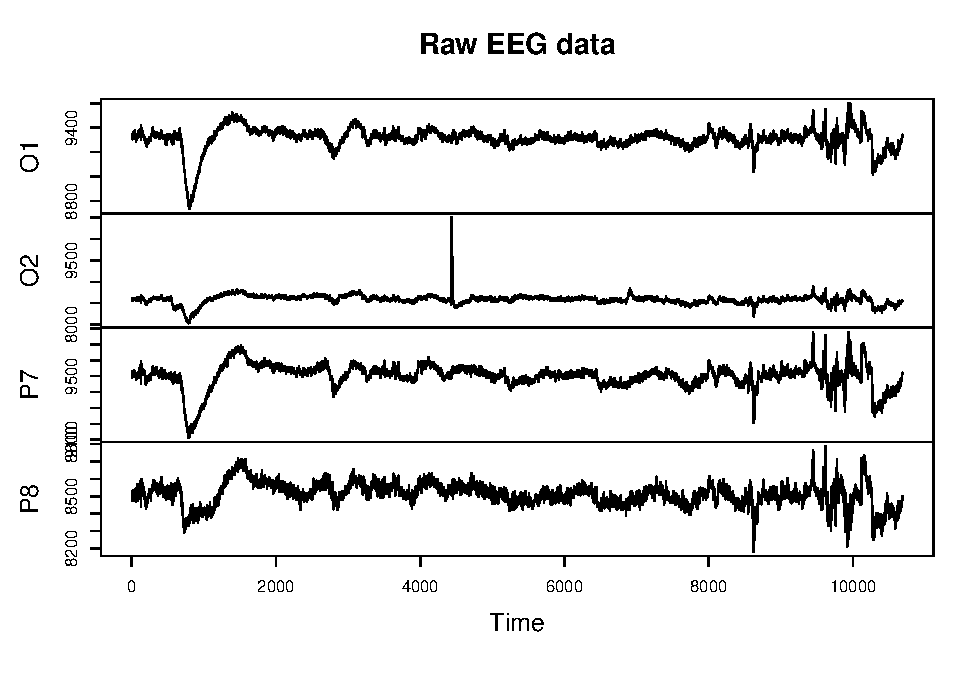
\includegraphics[width=30cm]{./img/eeg.pdf}};
	\coordinate [right of=eeg, node distance=39cm] (dummy2);
	\node [below of=dummy2, node distance=3cm, align=center] (dots) {$\bullet$\\$\bullet$\\$\bullet$};
	\coordinate [left of=dots, node distance=15.5cm] (dummy);
	\coordinate [left of=dummy2, node distance=15.5cm] (dummy3);
	\node [above of=dots] (cca) {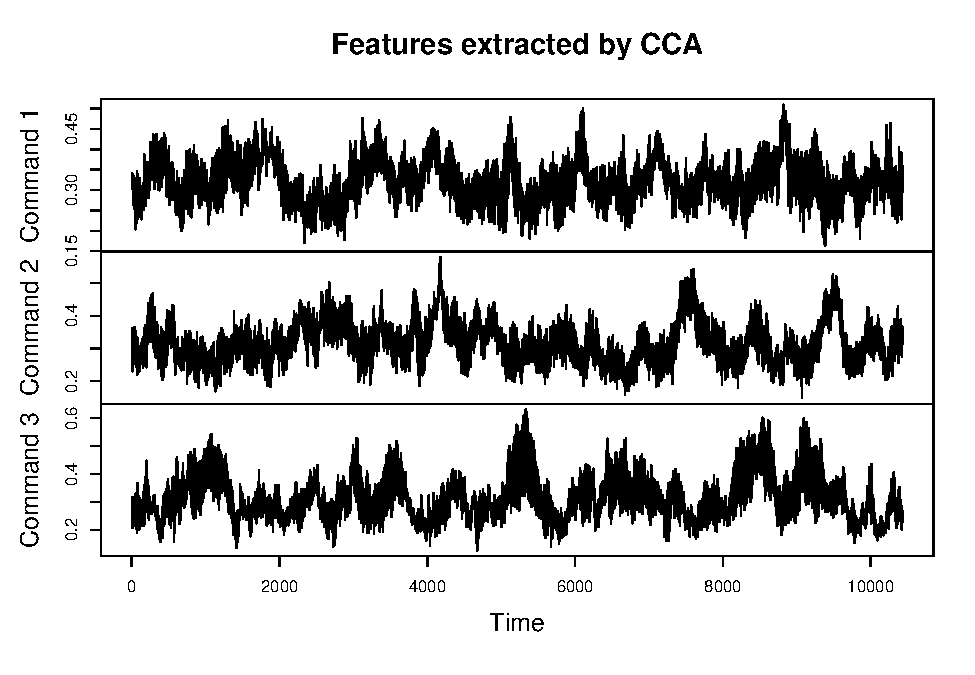
\includegraphics[width=30cm]{./img/cca_features.pdf}};
	\node [below of=dots] (psda) {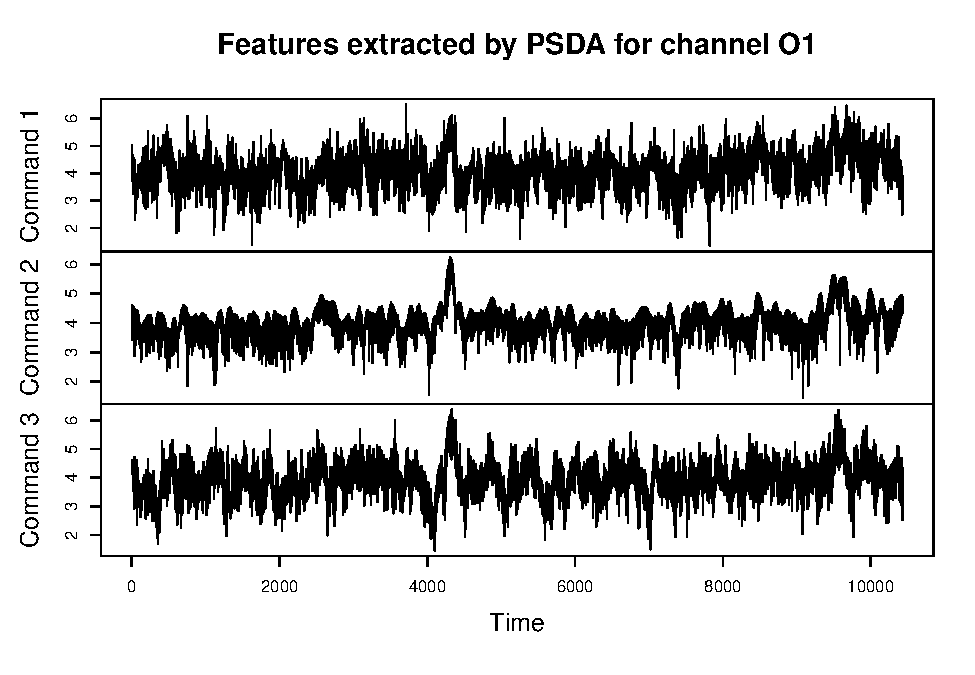
\includegraphics[width=30cm]{./img/psda_features.pdf}};

	\path [line] (eeg) -- (cca);
	\path [line] (eeg) -- (dummy);
	\path [line] (eeg) -- (dummy3);
	\path [line] (eeg) -- (psda);
	
%	% Arrows
%	\path [noArrow] (identification) -- (dummyRight);
%	\path [noArrow] (dummyRight) -- node [color=black, pos=0.5, above] {\textbf{visual feedback}} (dummyLeft);
%	\path [line] (dummyLeft) -- (monitor);
%	\path [line] (identification) -- node [color=black, above] {\textbf{command}} (robot);
%	\path [line] (extraction) -- (identification);
%	\path [line] (processing) -- (extraction);
%	\path [line] (emotiv) -- (processing);
%	\path [line] (brain) -- (emotiv);
	


\end{tikzpicture}

\end{textblock}

\begin{textblock}{10}(1.35, 6.1)
	\tikzstyle{decision} = [diamond, draw, fill=blue!20,
    text width=6em, text badly centered, inner sep=0pt]
\tikzstyle{block} = [rectangle, draw=Mat, fill=blue!20,
    text width=7em, text centered, rounded corners, minimum height=6em]
%\tikzstyle{line} = [draw, ultra thick, color=black!50, -latex']
\tikzstyle{line} = [draw=black,solid,line width=2mm,fill=black,
preaction={-triangle 90,ultra thick,draw,shorten >=-1mm}]
\tikzstyle{cloud} = [draw, ellipse,fill=red!20, 
    minimum height=2em]
%\tikzstyle{noArrow} = [draw, ultra thick, color=black!50]
\tikzstyle{noArrow} = [draw=black,solid,line width=2mm,fill=black]

\begin{tikzpicture}
	\draw[white, fill=white] (0,0) rectangle (1,1.5);
\end{tikzpicture}

\end{textblock}

\newcolumn
%\vspace{1cm}
\section{Introduction}
\begin{columns}[T]
	\column{0\textwidth}
	\column{0.98\textwidth}
\vspace{1.7cm}
\justify
The aim of this project is to improve the classification algorithm of a brain-computer interface (BCI) by using machine learning techniques. The BCI under consideration is author's previous work and therefore all the steps from data collection to classification were done either as a part ot this project or by using author's previous work. The BCI works by measuring users brain activity using electroencephalography (EEG) device Emotiv EPOC and then tries to find certain patterns from the EEG signal. In this case, the patterns we are interested in are changes in the amounts of frequencies present in the signal. But since brain signals are inherently very noisy and the EEG device used to collect data was a consumer-grade device, finding patterns in the signal turned out to be very challenging.
	\column{0.02\textwidth}
\end{columns}

\vspace{22.1cm}

\section{Factor structure}

\begin{columns}[T]
	\column{0.01\textwidth}
	\column{0.49\textwidth}
	\vspace{1.7cm}
	\begin{tabular}{|c|c|c|c|}\hline
		\phantom   & Factor 1 & Factor 2 & Factor 3\\\hline
		PSDA\_1 & \textbf{0.72}	  & 0.48	 & 0.27 \\\hline
		PSDA\_2 & 0.32	  & \textbf{0.75}	 & 0.31 \\\hline
		PSDA\_3 & 0.42	  & 0.41	 & \textbf{0.72} \\\hline
		CCA\_1 & \textbf{0.67}	  & -0.33	 & -0.14 \\\hline
		CCA\_2 & -0.15	  & \textbf{0.68}	 & -0.17 \\\hline
		CCA\_3 & -0.29	  & -0.40	 & \textbf{0.70} \\\hline
	\end{tabular}
	\column{0.48\textwidth}
	\justify
	\vspace{0.8cm}
	Before training classifiers, the data was analysed using exploratory factor analysis. The results showed that indeed there are similarities between the features that correspond to the same command. Features corresponding to same command were grouped into one factor. Detailed report is in repository.
\column{0.03\textwidth}
\end{columns}

\vspace{0.5cm}

\section{Machine learning algorithms}

\begin{columns}[T]
\column{0\textwidth}
\column{0.98\textwidth}
\vspace{1.7cm}
\justify
The multiclass classification task with three classes (commands) was divided into three binary classification tasks. Due to the noisiness of the data, stable learning algorithms were preferred. Many different learning algorithms were tested, including logistic regression, linear discriminant analysis, support vector machines (SVM) with different kernels, random forests and finally boosting, bagging and voting of different classifiers. The best results were achieved using soft voting of SVM and boosting of decision tree stumps. Final decision was made using the sum of the probabilities of the classes for given datapoint---if the sum of probabilities was larger than a given threshold, then the class was predicted. 

\column{0.02\textwidth}
\end{columns}

\newcolumn

\vspace{0.1cm}
\justify
To extract frequency information from the raw signal, canonical correlation analysis (CCA) and power spectral density analysis (PSDA) methods were used. These methods can be used to estimate how much certain frequency is present in the signal over some time window. During the data collection, users could send three different commands to the BCI and each command corresponds to some frequency change. CCA method extracts three different features from the data, one for each command. PSDA method, however, is not multidimensional and it extracts three features for each EEG channel (P7, O1, O2, P8).

\vspace{43.5cm}
\section{Results and conclusion}

\justify
In the figure below, the black dashed line denotes the expected state and the coloured lines denote the state predicted by the classifier on the test set. The thresholds were chosen so that there are no false positives. As can be seen the classifier is quite good at classifying command 2, but not so good at classifying command 3, which had the least training examples. Having high precision was preferred to filter out as many false positives as possible
\begin{columns}
	\column{0.01\textwidth}
	\column{0.615\textwidth}
	\justify
	The results are good starting point for further study. In this project, the classification algorithms only minimally took into account that we are predicting on time series, but the fact that observations are sequential in time contains very useful information and using it more should improve the performace of the classifiers.
	\column{0.02\textwidth}
	\column{0.37\textwidth}
	\begin{tabular}{|l||r|r|}
		\hline Command 2 & On & Off \\ 
		\hline\hline Predicted on & \textbf{514} & \textbf{45}\\ 
		\hline Predicted off\hspace{0.5cm} & \hspace{0.5cm}2751 & 4479 \\ 
		\hline
		\hline Command 1 & On & Off \\ 
		\hline\hline Predicted on &  \textbf{202} & \textbf{43}\\ 
		\hline Predicted off &  3106 & 4438 \\ 
		\hline
	\end{tabular}
\end{columns}

%NB THE TABLES SHOULD BE TRANSPOSED!!!!!!!!!!!!
%\begin{tabular}{|r||r|r||r|r||r|r|}
%%	\hline  &
%	\hline  & 1st on & 1st off & 2nd on & 2nd off & 3rd on & 3rd off\\ 
%	\hline Predicted on & 202 & 3106 & 514 & 2751 & 37 & 1179\\ 
%	\hline Predicted off & 43 & 4438 & 45 & 4479 & 52 & 6521\\ 
%	\hline Precision & 0.82 & & 0.92 & & 0.42 &\\
%	\hline
%\end{tabular}



\end{poster}
\end{document}